\documentclass[12pt]{article}
\usepackage{hyperref}
\usepackage{listings}
\usepackage[margin=1in]{geometry}
\usepackage{enumitem}
\usepackage{multicol}
\usepackage{array}
\usepackage{titlesec}
\usepackage{helvet}
\renewcommand{\familydefault}{\sfdefault}
\usepackage{amsmath}     % For math equations
\usepackage{amssymb}     % For advanced math symbols
\usepackage{amsfonts} % For math fonts
\usepackage{gvv}
\usepackage{esint}
\usepackage[utf8]{inputenc}
\usepackage{graphicx}
\usepackage{pgfplots}
\pgfplotsset{compat=1.18}
\titleformat{\section}{\bfseries\large}{\thesection.}{1em}{}
\setlength{\parindent}{0pt}
\setlength{\parskip}{6pt}
\usepackage{multirow}

\usepackage{fancyhdr}     % For custom headers and footers

\pagestyle{fancy}         % Use the fancy page style
\fancyhf{}                % Clear existing header/footer

% Header customization
\renewcommand{\headrulewidth}{0.4pt}          % Horizontal line at top
\fancyhead[L]{\textbf{2008}}                       % Page number on left
\fancyhead[R]{\textbf{ENGINEERING SCIENCES – XE}}  % Custom text on right
\cfoot{\thepage}

\usepackage[siunitx,RPvoltages]{circuitikz}
\usepackage{tikz}
\usepackage{float}
\usepackage{caption}
\begin{document}


\begin{center}

   \textbf{\large XE : Engineering Sciences} \\[1em]
    \textit{Maximum Marks: 150} \\[1em]
    \textbf{Duration: Three Hours}
\end{center}


\textbf{Read the following instructions carefully}
\begin{enumerate}
    \item This question paper contains 64 printed pages including pages for rough work. Please check all pages and report discrepancy, if any.

    \item Write your registration number, your name and name of the examination centre at the specified location on the right half of the ORS.

    \item Using HB pencil, darken the appropriate bubble under each digit of your registration number and the letters corresponding to your paper code.

    \item All the questions in this question paper are of objective type.

    \item Questions must be answered on Objective Response Sheet (ORS) by darkening the appropriate bubble (marked A, B, C, D) using HB pencil against the question number on the left hand side of the ORS. Each question has only one correct answer. If you wish to change an answer, erase the old one completely. More than one answer bubbled against a question will be treated as wrong answer.

    \item This question paper contains nine sections as listed below. \textbf{Section A is compulsory.} Choose any two sections from the remaining Sections B through H.
\end{enumerate}

\begin{center}
\begin{table}[H]     \centering     \caption{}     \label{}     \begin{tabular}{|c|l|c|}
    \hline
    \textbf{Section} & \textbf{Section Name} & \textbf{Page} \\
    \hline
    A & Engineering Mathematics & 03 \\
    \hline
    B & Computational Science & 08 \\
     \hline
    C & Electrical Sciences & 18\\
     \hline
    D & Fluid Mechanics & 32 \\
     \hline
    E & Materials Science & 44 \\
     \hline
    F & Solid Mechanics & 52 \\
     \hline
    G & Thermodynamics & 64 \\
     \hline
    H & Polymer Science and Engineering & 73 \\
     \hline
    I & Food Technology & 81 \\
    \hline
\end{tabular} \end{table}
\end{center}

\begin{enumerate}[start=7,label=\arabic*.]
    \item The XE Engineering Mathematics section (A), which is compulsory, carries 30 marks. Questions 1 through 8 are 2-mark questions. Questions 9 through 18 are 1-mark questions.

    \item Each of the other XE sections (B through I) carry 70 marks. Questions 1 through 8 are 1-mark questions; questions 9 through 32 (except Q32 and Q34) are 2-mark questions. Questions 32 and 34 are matching type with 2 marks each. Some of the questions may be linked.

    \item Un-attempted questions will carry zero marks.
\end{enumerate}

\textbf{NEGATIVE MARKING:}
\begin{itemize}
    \item \textbf{Section A:} For Q.1 to Q.6, 0.25 mark will be deducted for each wrong answer. For Q.7 to Q.18, 0.5 mark will be deducted for each wrong answer.

    \item \textbf{Sections B through I:} For Q.1 to Q.8, 0.25 mark will be deducted for each wrong answer. For Q.9 to Q.30, 0.66 mark will be deducted for each wrong answer. For linked questions, there will be negative marks only for the first question. For Q.31 and Q.34, 0.34 mark will be deducted. No negative marking for Q.32.
\end{itemize}

\begin{enumerate}[start=11,label=\arabic*.]
    \item Calculator \textbf{without data connectivity} is allowed in the examination hall.

    \item Charts, graph sheets and tables are \textbf{NOT} allowed in the examination hall.

    \item Rough work can be done on the question paper itself. Additional blank pages are given at the end of the question paper for rough work.
\end{enumerate}

\newpage



\begin{center}

   \textbf{\large A: ENGINEERING MATHEMATICS (\textit {Compulsary})} \\[1em]
    
\end{center}
\textbf{Q1-Q6 carry one mark each}

\begin{enumerate}
\item If the characteristic equation of a 3x3 matrix is $\lambda^3 - \lambda^2 + \lambda - 1 =0$, then the matrix should be 

\begin{enumerate}

\item  Hermitian 
\item Unitary
 \item Skew symmetric
\item Identity

\end{enumerate}

(GATE XE 2008)

\item {\large $\lim_{(x,y) \to (0,0)} \frac{x^4 + xy}{x^3 - y^3} $} is

\begin{enumerate}
\item 0
\item 1
\item -1
\item does not exist

\end{enumerate}
(GATE XE 2008)
\item If $f(z)= u + iv$ is an analytic function and $u-v=(x-y)^3 + kxy(x-y)$, then $k$ is

\begin{enumerate}
\item  2
\item  -4
\item  6
\item -8
\end{enumerate}

(GATE XE 2008)
\item The directional derivative at the point $P(1,2,3)$ to the surface {\large $x^2 + \frac{y^2}{4} + \frac{z^2}{9} =3$} in the direction of the vector $\overrightarrow{OP}$ ,where $O$ denotes the origin is

\begin{enumerate}
\item 0
\item {\Large $\frac{2}{\sqrt{14}}$}
\item {\Large $\frac{3}{\sqrt{14}}$}
\item {\Large $\frac{6}{\sqrt{14}}$}
\end{enumerate}

(GATE XE 2008)
\item If the solution of the differential equation $\frac{dy}{dx} + P(x)y = xy^3$ is $y^2(1+ce^{x^2}$, $c$ being an arbitary constant, then $P(x)$ is

\begin{enumerate}
\item  $-x$
\item  $\frac{x}{2}$
\item  $x$
\item $2x$
\end{enumerate}

(GATE XE 2008)
\item The system of equations \newline $ax+by+a^2=0$ \newline $bx+ay-b^2=0$ \newline $x+y+a-b=0$

\begin{enumerate}
\item  admits unique solution if $a=b\not =0$
\item admits unique solution if $a=-b\not=0$
\item admits unique solution if $a=b=0$
\item does not admit unique solution
\end{enumerate}

(GATE XE 2008)\newline
\textbf{Q7 to Q18 carry two marks each}
\item The matrix $\myvec{l&0&\sin\theta\\0&1&m\\n&0&\cos\theta}$ is orthogonal, if

\begin{enumerate}
\item $l=-\sin\theta, m=-\cos\theta, n=0$
\item $l=-\sin\theta, m=0, n=\cos\theta$
\item $l=\cos\theta, m=\sin\theta, n=0$
\item $l=-\cos\theta, m=0, n=\sin\theta$
\end{enumerate}

(GATE XE 2008)
\item The radius of convergence of the real power series $\sum_{m=0}^{\infty} \frac{(m!)^2}{(2m+1)!} x^m$ is

\begin{enumerate}
\item 4
\item  3
\item 2
\item 1
\end{enumerate}

(GATE XE 2008)
\item The value of \newline$(\int_{0}^{\frac{\pi}{2}} (\sin\theta)^\frac{3}{4} \, d\theta)$x$(\int_{0}^{\frac{\pi}{2}} (\sin\theta)^\frac{-3}{4} \, d\theta)$ is

\begin{enumerate}
\item $\frac{2\pi}{3} (\sqrt{2} +1)$
\item $\frac{2\pi}{3} (\sqrt{2} -1)$
\item $\frac{\pi}{2} (\sqrt{3})$
\item $\frac{-\pi}{2} (\sqrt{3})$
\end{enumerate}

(GATE XE 2008)
\item If $f(z)=y(1+x^2) +x^2 +i(y^2+2y)x$ is differentiable at a point $z=z_0$, then $f'(z_0)$ is

\begin{enumerate}
\item 0
\item 1
\item $i$
\item $-i$
\end{enumerate}

(GATE XE 2008)

\item  The value of the integral $\oint_{|z|=2} \frac{e^{1/z}}{(z-1)^2} \,dz$ is

\begin{enumerate}
\item 0
\item $(2e\pi)i$
 \item $(4e\pi)i$
\item $(4\pi)i$
\end{enumerate}

(GATE XE 2008)
\item  The absolute value of the integral $\oint_C(-zdx+xdy+ydz)$, where c is the curve obtained by the intersection of $x^2 + y^2 = a^2$and $y=z$, is

\begin{enumerate}
\item  $\frac{\pi a^2}{\sqrt{2}}$
\item $\frac{\pi a^2}{\sqrt{3}}$
\item $\pi a^2 \sqrt{2}$
\item $2\pi a^2$
\end{enumerate}

(GATE XE 2008)
\item  One of the values of  $\frac{1}{(4x^2D^2 + 8xD+1)}(\ln{x})$where $D\equiv \frac{d}{dx}$ is

\begin{enumerate}
\item  $\ln{x} +4$
\item $\ln{x} -4$
\item $4\ln{x} -4$
\item $4\ln{x} +4$
\end{enumerate}

(GATE XE 2008)
\item  A particular integral of the differential equation {\large $\frac{d^2y}{dx^2} - y = sec$ $h$ $x$} is

\begin{enumerate}
\item $- (cosh x) (ln cosh x) + xsinhx$
\item $- (sinh x) (Incosh x) + xcosh x$
\item $(cosh x) (Insinh x) + xsinh x$
\item $(sinh x) (ln cosh x) - x cosh x$
\end{enumerate}

(GATE XE 2008)
\item If $u=u(x,t)$ is such that $\frac{\partial^2 u}{\partial t^2} = 4\frac{\partial^2 u}{\partial x^2}$ , $0\leq x \leq \pi$ , $t \geq 0$, \newline $u(0,t)=u(\pi , t)=0,$\newline $u(x,0)=0,$ \newline $\frac{\partial u}{\partial t}(x,0)=\sin{x}$,\newline then $u(\frac{\pi}{3}, \frac{\pi}{6})$ is

\begin{enumerate}
\begin{multicols}{2}
\item $\frac{3}{4}$    
\item $\frac{\sqrt{3}}{4}$ 
\item $\frac{\sqrt{3}}{4}$
\item $\frac{\sqrt{3}}{8}$
\end{multicols}
\end{enumerate}


(GATE XE 2008)
\item The two lines of regression of the variables $x$ and $y$ are
$4x+2.4y = 20$ and $1.6x +4y =12$.
The coefficient of correlation between $x$ and $y$ is

\begin{enumerate}
\item 0.49
\item -0.49
\item  0.35
\item -0.35
\end{enumerate}

(GATE XE 2008)
\item While solving the initial value problem\newline $\frac{dy}{dx}+ky=0$, $y(0)=1$\newline at $x = h$ by fourth order Runge-Kutta method, the expression for $k_3$ is

\begin{enumerate}
\item  $-kh + \frac{(kh)^2}{2!} -\frac{(kh)^3}{3!}$
\item   $-kh + \frac{(kh)^2}{2} -\frac{(kh)^3}{3}$
\item   $-kh + \frac{(kh)^2}{2} -\frac{(kh)^3}{4}$
\item   $-k(1+\frac{h}{2}-\frac{h^2}{3})$
\end{enumerate}

(GATE XE 2008)
\item  On solving the system of equations\newline
$4x+z =5$\newline
$x+2y+3z =1$\newline
$-y-4z=3,$\newline
by $LU$ - decomposition with $u_{ii} =1$ for i =1,2,3; the values of $u_{23}$ and $l_{33}$ are respectively

\begin{enumerate}
\item  1.375 and -4.250
\item  2.750 and -3.625
\item  1.375 and -2.625
\item 2.750 and -4.250
\end{enumerate}

(GATE XE 2008)\


\end{enumerate}
    
 

\begin{center}
   
    \textbf{END OF SECTION - A}
\end{center}
\newpage
\begin{center}
    \textbf{B:COMPUTATIONAL SCIENCE}
\end{center}


\begin{enumerate}
\item[] \textbf{Q1-Q8 carry one mark each}
\item  Which one of the following is not a physical component of a computer ?

\begin{enumerate}

\item  CPU 
\item  RAM
\item  Assembler 
\item  Motherboard
\end{enumerate}

(GATE XE 2008)
\item A number whose representation in base \textit{b}  is 64, is equal to 100 in the decimal representation. The value of the base \textit{b} is

\begin{enumerate}
\begin{multicols}{4}
\item 4
\item 8
\item 12
\item 16
\end{multicols}
\end{enumerate}

(GATE XE 2008)
\item Evaluation of the integral \newline {\Large$\int_{1}^{2} \frac{dx}{\sqrt{1+x^2}}$}\newline using 2 segment trapezoidal rule with equal intervals gives the result

\begin{enumerate}
\begin{multicols}{4}
\item 0.566
\item 0.564
\item 0.562
\item 0.560
\end{multicols}
\end{enumerate}

(GATE XE 2008)
\item A continuous function $f(x)$ defined in interval [a,b] is such that $f(a)f(b)<0$.A possible number of simple roots of the equation $f(x)=0$ in this interval is

\begin{enumerate}
\begin{multicols}{4}
\item 0
\item 1
\item 2
\item 4
\end{multicols}
\end{enumerate}

(GATE XE 2008)
\item The function $e^x$ is expanded about the point $x=0$ in a Taylor polynomial $P_{n}(x)$ of degree $n$. The value of $n$ necessary to approximate $e^x$ to an accuracy of $10^{-5}$ in [0,0.5] is

\begin{enumerate}
\begin{multicols}{4}
\item 5
\item 6
\item 7
\item 8
\end{multicols}
\end{enumerate}

(GATE XE 2008)
\item The eigenvalues of the matrix $\begin{pmatrix}0&-1\\1&0\end{pmatrix}$ are\newline

\begin{enumerate}
\begin{multicols}{2}
\item 1,-1          
\item $i,i$
\item 1,1    
\item $i,-i$
\end{multicols}
\end{enumerate}

(GATE XE 2008)
\item  Consider the following code segment in Fortran:
\begin{verbatim}
   REAL PARAMETER:: X=10.0, Y=2.0, Z=5.0
   REAL:: RESULT
   RESULT = X/Y+Y*Z**2
\end{verbatim}
The value of the result when this code segment is executed, is

\begin{enumerate}
\begin{multicols}{2}
\item 0.098  
\item 0.192
\item 55.0   
\item 105.0
\end{multicols}
\end{enumerate}

(GATE XE 2008)
\item The value of the integral $\int_{1}^{2} \frac{dx}{x}$ obtained by using Simpson's 1/3 rule, with 3 points, is

\begin{enumerate}
\begin{multicols}{4}
\item 0.694 
\item 0.693 
\item 0.692 
\item 0.691
\end{multicols}
\end{enumerate}

(GATE XE 2008)

\item []\textbf{Q9 to Q30 carry two marks each}
\item  The hypotenuse \textit{c} and a side \textit{b} of a right triangle are found by measurement to be 13 cm and 5 cm respectively. The possible error in the measurement of the hypotenuse is 0.2 cm and that in the side \textit{b} is 0.1 cm. The maximum possible error (in cm) in the calculation of the third side is

\begin{enumerate}
\begin{multicols}{4}
\item 0.26 
\item 0.22 
\item 0.17 
\item 0.10
\end{multicols}
\end{enumerate}

(GATE XE 2008)
\item One of the eigenvalues of a 3×3 matrix $M$ is 3. If the determinant of the matrix $M$ is 24 and the trace is 9, then the smallest eigenvalue of the matrix $M^{-1}$ is

\begin{enumerate}
\begin{multicols}{4}
\item 1/8 
\item 1/4 
\item 1/3 
\item 1/2
\end{multicols}
\end{enumerate}

(GATE XE 2008)
\item  A quadrature formula is given by\begin{center} $\int_{0}^{1} f(x) \,dx =pf(0) + qf(0.5) +rf(1)$\end{center} where the coefficients $p,q$ and $r$ rare determined by comparing the right hand side of the above formula with the exact value of the integral for a quadratic polynomial. The formula corresponds to

\begin{enumerate}
\item Two segment trapezoidal rule
\item One segment trapezoidal rule
\item Simpson's 3/8 rule
\item Simpson's 1/3 rule
\end{enumerate}

(GATE XE 2008)
\item The set of simultaneous equations \begin{center}$4x-y=15$ 

$x+5y=9$\end{center} is to be solved using Jacobi's iterative method. Starting with the initial values x = 2, y =2, the values of x and y after two iterations are, respectively,

\begin{enumerate}
\begin{multicols}{2}
\item  4.25, 0.95
\item  4.25, 1.4
\item  4.1, 0.95
\item 4.1, 1.4
\end{multicols}
\end{enumerate}

(GATE XE 2008)
\item The lower triangular matrix $L$ in the LU factorization of the matrix\newline
$\begin{pmatrix}
    25&5&4\\10&8&16\\8&10&22
\end{pmatrix}$ is written as $\begin{pmatrix}
    1&0&0\\L_{21}&1&0\\L_{31}&L_{32}&1
\end{pmatrix}$. The element $L_{32}$ is 

\begin{enumerate}
\begin{multicols}{4}
\item 1.0 
\item 1.4 
\item 0.4 
\item 0.32
\end{multicols}
\end{enumerate}

(GATE XE 2008)
\item For a function $f(x)$ whose second derivative $f"(x)$ has a maximum value 12 in the interval [0,1]. The number of segments required to integrate $\int_{0}^{1} f(x) \,dx$
with an accuracy of 0.001 using trapezoidal rule is

\begin{enumerate}
\begin{multicols}{4}
\item  10 
\item  12
\item 100 
\item 1000
\end{multicols}
\end{enumerate}

(GATE XE 2008)
\item  An approximate solution of the equation $x^3 - 3x+1=0$ is 0.347296. Which of the following iterating functions will converge most rapidly to this root?

\begin{enumerate}
\begin{multicols}{2}
\item  $x_{n+1} = \frac{1}{(3-x_{n}^2)}$
\item  $x_{n+1}=\frac{1}{3}(x_{n}^3 + 1)$
\item  $x_{n+1}=\frac{1}{5}(x_{n}^3 +2x_{n}+ 1)$
\item  $x_{n+1}=\frac{1}{27}(10x_{n}^3 -3x_{n} + 10)$
\end{multicols}
\end{enumerate}

(GATE XE 2008)
\item  A real root of the equation $x^3 -2x-5 =0$ lies between $x=2$ and $x = 3$. The location of the root obtained after the second iteration using the method of false position is

\begin{enumerate}
\begin{multicols}{4}
\item  2.081 
\item 2.061 
\item  2.059 
\item 2.041
\end{multicols}
\end{enumerate}

(GATE XE 2008)
\item The solution of the first order differential equation $(0\leq x\leq1)$\newline
$\frac{dy}{dx} - y^2 =0$ with $y(0)=1$ is

\begin{enumerate}
\begin{multicols}{2}
\item  $\frac{1}{1+x}$  
\item  $\frac{1}{1-x}$
\item  $\frac{2}{2+x}$  
\item $\frac{x^3}{3} +1$
\end{multicols}
\end{enumerate}

(GATE XE 2008)
\item  For the initial value problem\newline
$\frac{dy}{dx}+y=0 , y(0)=1 , y_{1}$  is the computed value of $y$ at $x = 0.2$ obtained by using Euler's $dx$ method with step size $h =0.1$. Then,

\begin{enumerate}
\begin{multicols}{2}
\item $y_{1} < e^{-0.2}$  
\item  $e^{-0.2}<y_{1}<1$
\item  $1<y_{1}$       
\item $y_{1}=e^{-0.2}$
\end{multicols}
\end{enumerate}

(GATE XE 2008)
\item Consider the initial value problem\newline
$\frac{dy}{dx}=y+x$ with $y(0)=2$.\newline
The value of $y(0.1)$ obtained using the fourth order Runge-Kutta method with step size $h = 0.1$ is

\begin{enumerate}
\begin{multicols}{4}
\item  2.20000 
\item 2.21500 
\item 2.21551 
\item 2.21576
\end{multicols}
\end{enumerate}

(GATE XE 2008)
\item The following table gives a function $f(x)$ vs $x$\newline
\begin{table}[H]     \centering     \caption{}     \label{}     \begin{tabular}{|c|c|c|c|c|c|}
\hline
    $x$ & 0 & 1 & 2 & 3 & 4 \\
    \hline
    $f(x)$ & 1.0 & 3.7 & 6.5 & 9.3 & 12.1\\
    \hline
\end{tabular} \end{table}
The best fit of a straight line for the above data points, using a least square error method is

\begin{enumerate}
\begin{multicols}{2}
\item  2.75$x$+0.55
\item  2.80$x$+0.80
\item  3.10$x$+0.85
\item 2.78$x$+0.96
\end{multicols}
\end{enumerate}

(GATE XE 2008)

\item Consider the following part of a Fortran 90 function \begin{verbatim}
    INTEGER FUNCTION RESULT (X)
        INTEGER::X
        VALUE =1
        DO
            IF (X == 0) EXIT
            TERM = MOD (X,10)
            VALUE = VALUE*TERM
            X = X/10
        END DO
        RESULT = VALUE
    END FUNCTION RESULT
\end{verbatim}
If the above function is called with an integer $X=123$, the value returned by the function will be

\begin{enumerate}
\begin{multicols}{4}
\item  0 
\item 6 
\item 9 
\item 321
\end{multicols}
\end{enumerate}

(GATE XE 2008)
\item  A portion of a Fortran 90 program is reproduced below:
\begin{verbatim}
    PROGRAM CHECK_CYCLE
        DO I =1, 10, 2
            IF (MOD(I, 3) == 0 ) CYCLE
            PRINT *, I
        END DO
    END PROGRAM CHECK_CYCLE
\end{verbatim}
The result displayed by the program is

\begin{table}[H]     
\centering     
\caption{}     
\label{}     
\begin{tabular}{ll}
(a) & 
    \begin{tabular}{l}
1 \\
5 \\
7
\end{tabular}  
\\
\\
(b) & 
     \begin{tabular}{l}
1 \\
3 \\
5
\end{tabular} 
\\
\\
(c) & 
    \begin{tabular}{l}
1 \\
3 \\
7
\end{tabular} \\
\\
(d) & 
    \begin{tabular}{l}
3 \\
5 \\
7
\end{tabular} 

\end{tabular} \end{table}

(GATE XE 2008)
\item (P), (Q), (R) and (S) are separate segments of Fortran 90 code.
\begin{verbatim}
    (P) IF (A > B) P=Q
    (Q) SUBROUTINE SWAP(A, B)
        INTEGER, INTENT(IN):: A, B
        TEMP = A
        A = B
        B = TEMP
        END SUBROUTINE SWAP
    (R) IF (A /= B) X = Y-Z
        ELSE
          X=Y+Z
        ENDIF
    (S) DO I = 1, N, 3
          C(I) = A(I) + B(I)
        END DO
\end{verbatim}

Which segments have syntax errors?

\begin{enumerate}
\begin{multicols}{4}
\item  P, Q 
\item  Q, R 
\item  R, S 
\item P,S
\end{multicols}
\end{enumerate}

(GATE XE 2008)
\item A Fortran-90 subroutine for Gauss-Siedel Method to solve a set of N simultaneous equations $[A][X]=[C]$ is given below.
\begin{verbatim}
 SUBROUTINE SIEDEL(A, C, X, N,
 IMAX)
 REAL:: SUM
 REAL, DIMENSION(N,N):: A
 REAL, DIMENSION(N):: C, X
  DO K = 1, IMAX
    DO I = 1, N
        SUM = 0.0
        DO J = 1, N
            IF ( I / = J ) THEN
              SUM=SUM+A(I,J)*X(J)
            ENDIF
        ENDDO
        ******
    ENDDO
  ENDDO
 END SUBROUTINE SIEDEL
\end{verbatim}

The missing statement in the program, indicated by ******, is

\begin{enumerate}
\item  \texttt{X(I) C(I) + SUM}

\item  \texttt{X(I) = C(I) - SUM}

\item  \texttt{X(I) = (C(I) + SUM)/A(I,I)}

\item  \texttt{X(I) = (C(I) - SUM)/A(I,I)}
\end{enumerate}

(GATE XE 2008)
\item  What is the result of the following C program?
\begin{verbatim}
    int main()
    {
       int i, sum=0;
       for (i = 0; i < 25; i++ ) {
          if (i > 10 ) continue;
          sum += i;
       }
       printf("%d\n", sum);
       return 1;
    }   
\end{verbatim}

\begin{enumerate}
\begin{multicols}{4}
\item  25  
\item  45  
\item  55 
\item  325
\end{multicols}
\end{enumerate}

(GATE XE 2008)
\item  Consider the following C code.
\begin{verbatim}
    int x = 1, y = 5, z;
    z = x++<<--y;

\end{verbatim}
The values of x,y and z after the execution are

\begin{enumerate}
\begin{multicols}{4}
\item  2,4,16  
\item  2,4,32
\item 2,4,64   
\item 1,5,32
\end{multicols}
\end{enumerate}

(GATE XE 2008)
\item A two dimensional array is declared as \texttt{int num[3] [3]}. Then the result of the expression \texttt{* (num+1)} is

\begin{enumerate}
\item The value of \texttt{num[1][0]}

\item  The value of \texttt{num[0][1]}

\item  The address of \texttt{num[1][0]}

\item  The address of \texttt{num[0][1]}
\end{enumerate}

(GATE XE 2008)
\item A C function named \texttt{func} is defined as follows:
\begin{verbatim}
int func(int a, int b) {
    if ( (a == 1)||(b == 0)||
         (a == b) ) return 1;
    return func(a-1,b)+func(a-1,b-1);
}

\end{verbatim}
What is the result of \texttt{func (4,2)}?

\begin{enumerate}
\begin{multicols}{4}
\item  $12$  
\item  $6$  
\item  $3$  
\item $1$
\end{multicols}
\end{enumerate}

(GATE XE 2008)
\\
\\

\noindent \textbf{\large Common Data Questions}

\textbf{Common data for questions 29 and 30: }

The following table gives the values of a function f at three discrete points.

\begin{table}[H]     \centering     \caption{}     \label{}     \begin{tabular}{|c|c|c|c|}
    \hline
    $x$ & $0.5$ & $0.6$ & $0.7$ \\
    \hline
    $f(x)$ & $0.4794$ & $0.5646$ & $0.4662$ \\
    \hline
\end{tabular} \end{table}
\item The value of $f'(x)$ at $x = 0.5$ accurate upto two decimal places, is

\begin{enumerate}
\begin{multicols}{2}
\item  $0.82$
\item  $0.85$
\item  $0.88$
\item  $0.91$
\end{multicols}
\end{enumerate}

(GATE XE 2008)
\item  The value of $f'(x)$ at $x =0.55$ obtained using Newton's interpolation formula, is

\begin{enumerate}
\begin{multicols}{2}
\item  $0.5626$
\item  $0.5227$
\item  $0.4847$
\item  $0.4749$
\end{multicols}
\end{enumerate}

(GATE XE 2008)
\\
\\
\noindent \textbf{\large Linked Answer Questions: Q31 to Q34 carry two marks each.}

\textbf{Statement for Linked Answer Questions 31 and 32:}

A modified Newton-Raphson method is used to find the roots of an equation $f(x)= 0$ which has multiple zeros at some point $x = p$ in the interval $[a,b]$. If the multiplicity $M$ of the root is known in advance, an iterative procedure for determining $p$ is given by \newline \\
$p_{k+1} = p_{k} - M\frac{f(p_{k})}{f'(p_{k})}$ for $k=0,1,2,...$
\\
\item  The equation $f(x)=x^2-1.8x^2 -1.35x+2.7= 0$ is known to have a multiple root in the
interval $[1,2]$. Starting with an initial guess $x =1.0$ in modified Newton-Raphson method, the root, correct up to three decimal places, is

\begin{enumerate}
\begin{multicols}{2}
\item  $1.500$
\item  $1.200$
\item  $1.578$
\item  $1.495$
\end{multicols}
\end{enumerate}

(GATE XE 2008)

\item The root of the derivative of $f(x)$ in the same interval is

\begin{enumerate}
\begin{multicols}{2}
\item  $1.500$ 
\item  $1.200$
\item  $1.578$ 
\item  $1.495$
\end{multicols}
\end{enumerate}

(GATE XE 2008)
\\ \\
\textbf{Statement for Linked Answer Questions 33 and 34:}

The values of a function $f(x)$ at four discrete points are as follows:
\begin{center}
\begin{table}[H]     \centering     \caption{}     \label{}     \begin{tabular}{|c|c|c|c|c|}
\hline
   $x$  & $0$ & $1$ & $2$ & $4$\\
   \hline
  $f(x)$   & $-12$ & $0$ & $6$ & $12$\\
  \hline
\end{tabular} \end{table}
\end{center}

\item  The function may be represented by a polynomial $P(x)=(x-a)R(x)$, where $R(x)$ is a polynomial of degree $2$, obtained by Lagrange's interpolation and a is a real constant. The polynomial $R(x)$ is

\begin{enumerate}
\item  $x^2+6x+12$
\item  $x^2+6x-12$
\item  $x^2-6x-12$
\item  $x^2-6x+12$
\end{enumerate}

(GATE XE 2008)
\item The value of the derivative of the interpolated polynomial $P(x)$ at the position of its real root is

\begin{enumerate}
\begin{multicols}{4}
\item  $-6$
\item  $-4$
\item  $6$
\item  $7$
\end{multicols}
\end{enumerate}

(GATE XE 2008)







\end{enumerate}
    


\begin{center}
    \textbf{END OF SECTION-B}
\end{center}

\newpage
\begin{center}
    \textbf{C:ELECTRICAL SCIENCES}
\end{center}



\begin{enumerate}
\item[] \textbf{Q1 - Q8 carry one mark each}

\item  An LC circuit is shown in the figure. The inductor current, i, when the switch S is opened at t = 0 is best represented by

    

\begin{figure}[H]
\centering
\resizebox{0.3\columnwidth}{!}{%
\begin{circuitikz}
\tikzstyle{every node}=[font=\LARGE]
\draw (3.5,14) to[short] (4.25,14);
\node at (4.25,14) [circ] {};
\draw (4.25,14) to[opening switch] (5.75,14);
\node at (5.75,14) [circ] {};
\node at (5.75,14) [circ] {};
\draw (5.75,14) to[short] (6.5,14);
\draw (3.5,14) to[short] (3.5,12);
\draw (6.5,14) to[short] (6.5,12);
\draw (3.5,12) to[L ] (6.5,12);
\draw (3.5,12) to[curved capacitor] (3.5,10);
\draw (3.5,10) to[short] (6.5,10);
\draw (6.5,12) to[short] (6.5,10);
\draw [->, >=Stealth] (3.5,12) -- (4.25,12);
\node [font=\large] at (5,14.5) {t=0};
\node [font=\large] at (5,13.5) {S};
\node [font=\large] at (5,12.5) {i(0)=10A};
\node [font=\large] at (2.5,11) {v(0)=0};
\node [font=\large] at (4,11) {C};
\node [font=\normalsize] at (4,12.25) {i};
\end{circuitikz}
}%
\caption{}
\label{fig:my_label}
\end{figure}


\begin{multicols}{2}
(a) \begin{figure}[H]
  \centering
  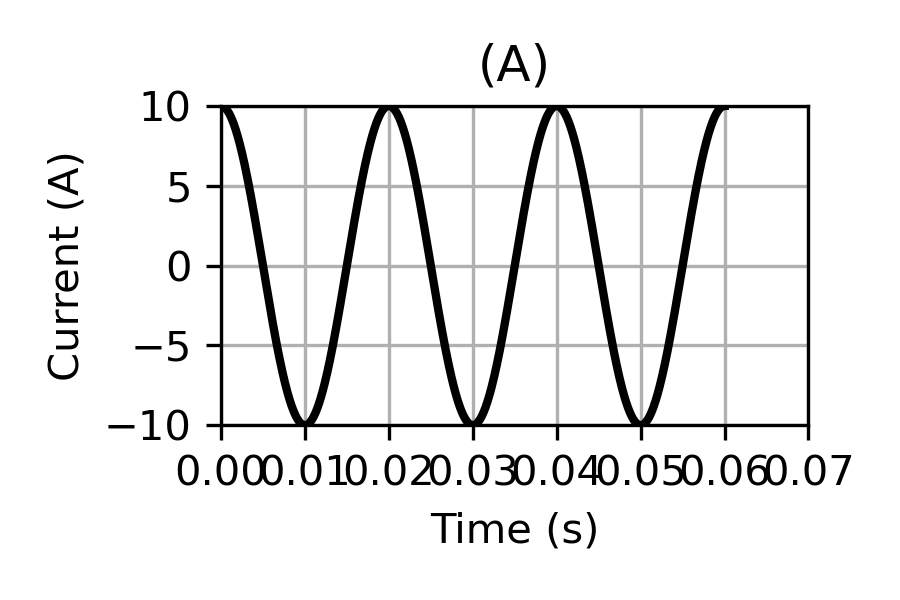
\includegraphics[width=0.7\columnwidth]{figs/cosine_wave2.png}
  \caption{}
\end{figure}

(b) \begin{figure}[H]
  \centering
  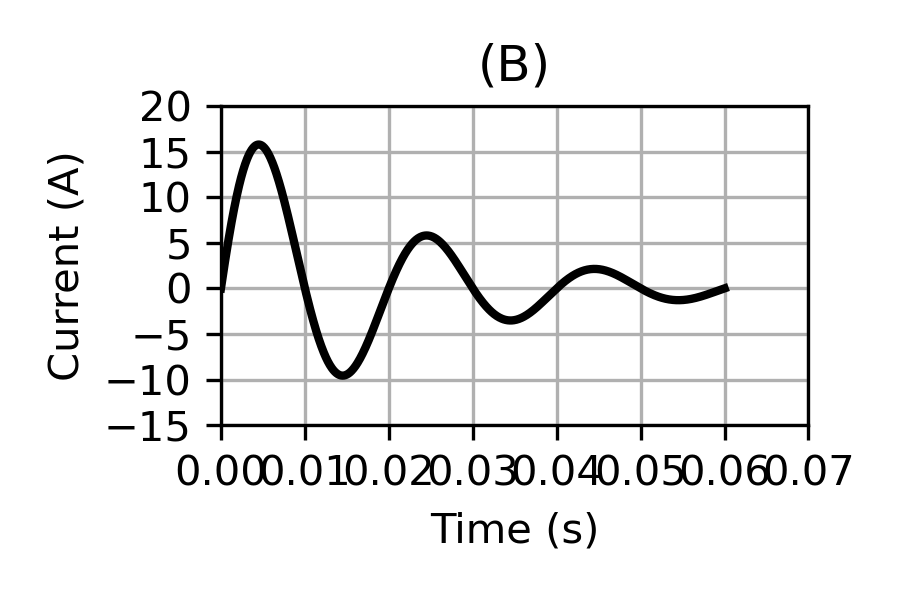
\includegraphics[width=0.7\columnwidth]{figs/damped_sine_wave1.png}
  \caption{}
\end{figure}

(c) \begin{figure}[H]
  \centering
  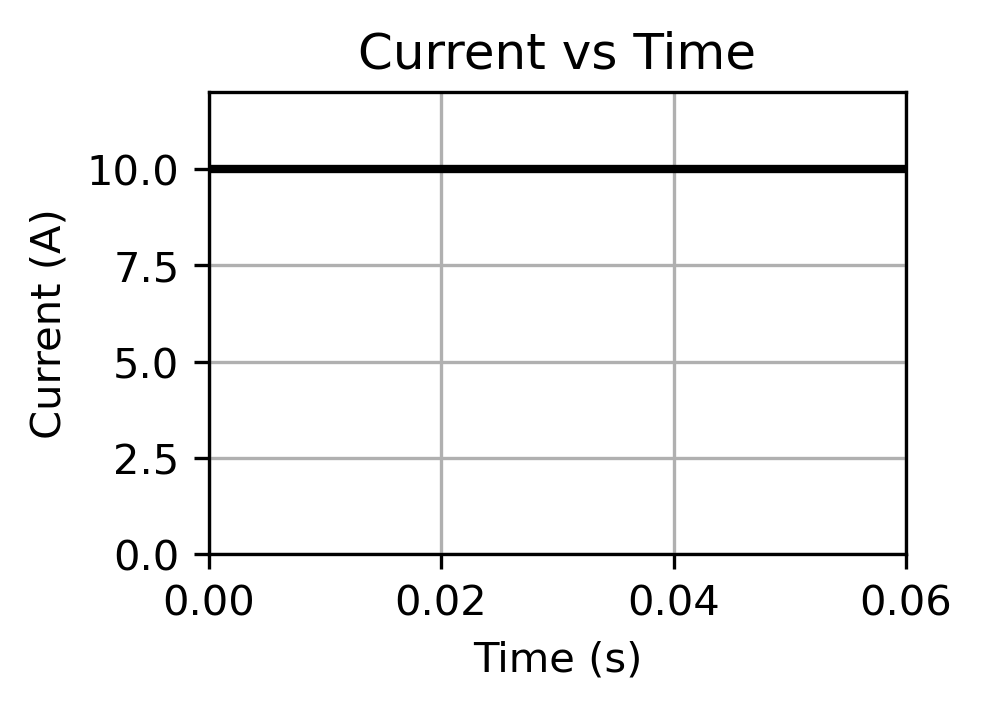
\includegraphics[width=0.7\columnwidth]{figs/constant_wave.png}
  \caption{}
\end{figure}

(d) \begin{figure}[H]
  \centering
  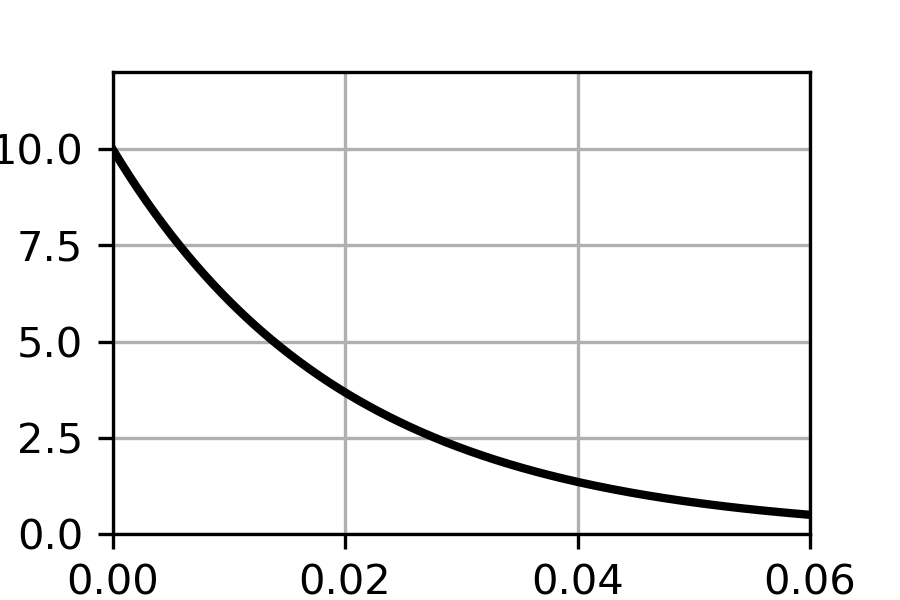
\includegraphics[width=0.7\columnwidth]{figs/exponential_current_rise.png}
  \caption{}
\end{figure}


\end{multicols}


(GATE XE 2008)


\item In the figure shown, power supplied by the current source is

\begin{figure}[H]
\centering
\resizebox{0.2\columnwidth}{!}{%
\begin{circuitikz}
\tikzstyle{every node}=[font=\LARGE]
\draw (3.25,12.75) to[battery1] (5,12.75);
\draw (5,12.75) to[R] (6.5,12.75);
\draw (6.5,11.25) to[american current source] (3.25,11.25);
\draw (3.25,12.75) to[short] (3.25,11.25);
\draw (6.5,12.75) to[short] (6.5,11.25);
\node [font=\Large] at (4,13.25) {10V};
\node [font=\Large] at (5.75,13.25) {2.5$\Omega$};
\node [font=\Large] at (4.75,10.5) {2A};
\end{circuitikz}
}%
\caption{}
\label{fig:my_label}
\end{figure}

\begin{enumerate}
\begin{multicols}{2}
\item $0.0 W$
\item $5.0 W$, delivered
\item $10.0 W$, delivered
\item  $10.0 W$, absorbed
\end{multicols}
\end{enumerate}

(GATE XE 2008)
\item An inductor of $0.4$ H was constructed with $20$ turns on an iron core. If $10$ additional turns in the same sense are added to the coil on the same core, the new inductance will be

\begin{enumerate}
\begin{multicols}{4}
\item  $0.9 H$ 
\item  $0.8 H$ 
\item  $0.7 H$ 
\item  $0.6 H$
\end{multicols}
\end{enumerate}

(GATE XE 2008)
\item  A three-phase star-connected, slip-ring induction motor has per-phase standstill rotor resistance, $r_{2} = 0.01$ and reactance, $x_{2} = 0.05$ . To achieve maximum torque at starting, the external perphase resistance to be connected at the slip-rings is

\begin{enumerate}
\begin{multicols}{4}
\item  $0.01 \Omega$ 
\item  $0.02 \Omega$ 
\item  $0.03 \Omega$ 
\item  $0.04 \Omega$
\end{multicols}
\end{enumerate}

(GATE XE 2008)
\item  The device structure shown in the figure is that of a

\begin{figure}[H]
\centering
\resizebox{0.3\columnwidth}{!}{%
\begin{circuitikz}
\tikzstyle{every node}=[font=\large]
\draw  (3.25,12.75) rectangle (5.25,12.25);
\draw [short] (4.75,12.75) -- (4.75,13.25);
\draw [short] (4.75,13.25) -- (5.75,13.25);
\draw [short] (5.75,13.25) -- (5.75,12.25);
\draw [short] (5.25,12.25) -- (5.75,12.25);
\draw  (5.75,12.75) rectangle (9.25,12.25);
\draw  (6,13.25) rectangle (9,12.75);
\draw [short] (9.25,12.75) -- (9.25,13.25);
\draw [short] (9.25,13.25) -- (10.75,13.25);
\draw [short] (10.75,13.25) -- (10.75,12.75);
\draw  (9.75,12.75) rectangle (12,12.25);
\draw  (4.75,12.25) rectangle (6.5,11.5);
\draw  (9,12.25) rectangle (11,11.5);
\begin{scope}[rotate around={-97.25:(3.25,12.25)}]
\draw[domain=3.25:5.25,samples=100,smooth] plot (\x,{0.2*sin(8.1*\x r -3.25 r ) +12.25});
\end{scope}
\begin{scope}[rotate around={-90:(12,12.25)}]
\draw[domain=12:14,samples=100,smooth] plot (\x,{0.3*sin(7.58*\x r -12 r ) +12.25});
\end{scope}
\draw [short] (3,10.25) -- (12.25,10.25);
\draw [short] (3,10.25) -- (2.75,10.25);
\node at (5,14) [circ] {};
\node at (5,14) [circ] {};
\node at (5,14) [circ] {};
\node at (7.5,14) [circ] {};
\node at (10,14) [circ] {};
\draw (5,14) to[short] (5,13.25);
\draw (7.5,14) to[short] (7.5,13.25);
\draw (10,14) to[short] (10,13.25);
\draw [->, >=Stealth] (8.25,11.5) -- (8,12.25);
\node [font=\LARGE] at (5,14.5) {$V_S$};
\node [font=\LARGE] at (7.5,14.5) {$V_G$};
\node [font=\LARGE] at (10,14.5) {$V_D$};
\node [font=\Large] at (5.5,12) {$P$};
\node [font=\Large] at (10,12) {$P$};
\node [font=\large] at (8.25,11.25) {$oxide$};
\node [font=\Large] at (5.5,10.75) {$n substrate$};
\end{circuitikz}
}%
\caption{}
\label{fig:my_label}
\end{figure}

\begin{enumerate}
\begin{multicols}{2}
\item  pnp BJT
\item  p-channel MOSFET
\item  npn BJT
\item  n-channel MOSFET
\end{multicols}
\end{enumerate}

(GATE XE 2008)
\item  The input voltage applied to the rectifier circuit shown in the figure is $V_{in} = V_{m} sin(2\pi50t)$. The steady state output voltage $V_{o}$ of the rectifier, under no-load condition, is

\begin{figure}[H]
\centering
\resizebox{0.3\columnwidth}{!}{%
\begin{circuitikz}
\tikzstyle{every node}=[font=\large]
\draw (4.75,12) to[sinusoidal voltage source, sources/symbol/rotate=auto] (4.75,11);
\draw (4.75,12) to[short] (6.25,12);
\draw (4.75,11) to[crossing] (7.75,11);
\draw (6.25,12) to[D] (6.25,14);
\draw (6.25,8.5) to[D] (6.25,12);
\draw (7.75,11) to[curved capacitor] (7.75,8.5);
\draw (7.75,14) to[curved capacitor] (7.75,11);
\draw (6.25,8.5) to[short] (8.75,8.5);
\draw (6.25,14) to[short] (8.25,14);
\draw (8.25,14) to[short] (8.75,14);
\node at (8.75,14) [circ] {};
\node at (8.75,8.5) [circ] {};
\node [font=\large] at (4,11.5) {$V_{in}$};
\node [font=\large] at (9,11.25) {$V_o$};
\node [font=\large] at (8.75,13.5) {$+$};
\node [font=\large] at (8.75,8.75) {$-$};
\end{circuitikz}
}%
\caption{}
\label{fig:my_label}
\end{figure}

\begin{enumerate}
\begin{multicols}{4}
\item  $V_m$ 
\item $\sqrt{2} V_m$ 
\item  $2 V_m$ 
\item  $2\sqrt{2} V_m$
\end{multicols}
\end{enumerate}

(GATE XE 2008)
\item In the figure shown, the diode is ideal and the zener voltage is $10 V$. The input voltage, $v_{in} =10\sqrt{2} (100\pi t) V$. The wave-shape of the current through the resistor, R is represented by

\begin{figure}[H]
\centering
\resizebox{0.3\columnwidth}{!}{%
\begin{circuitikz}
\tikzstyle{every node}=[font=\large]
\draw (3.5,14.25) to[sinusoidal voltage source, sources/symbol/rotate=auto] (3.5,11.5);
\draw (3.5,14.25) to[D] (7,14.25);
\draw (7,12.5) to[empty Zener diode] (7,14.25);
\draw (7,12.5) to[R] (7,11.25);
\draw (3.5,11.5) to[short] (3.5,10.75);
\draw (7,11.25) to[short] (7,10.75);
\draw (3.5,10.75) to[short] (7,10.75);
\node [font=\large] at (2.75,13) {$V_{in}$};
\node [font=\large] at (5.25,14.75) {$D$};
\node [font=\large] at (7.75,13.25) {$10V$};
\node [font=\large] at (8,11.75) {$R=1\Omega$};
\node [font=\large] at (7.25,13.75) {$+$};
\node [font=\large] at (7.25,13) {$-$};
\end{circuitikz}
}%
\caption{}
\label{fig:my_label}
\end{figure}

\begin{multicols}{2}
(a) \begin{figure}[H]
  \centering
  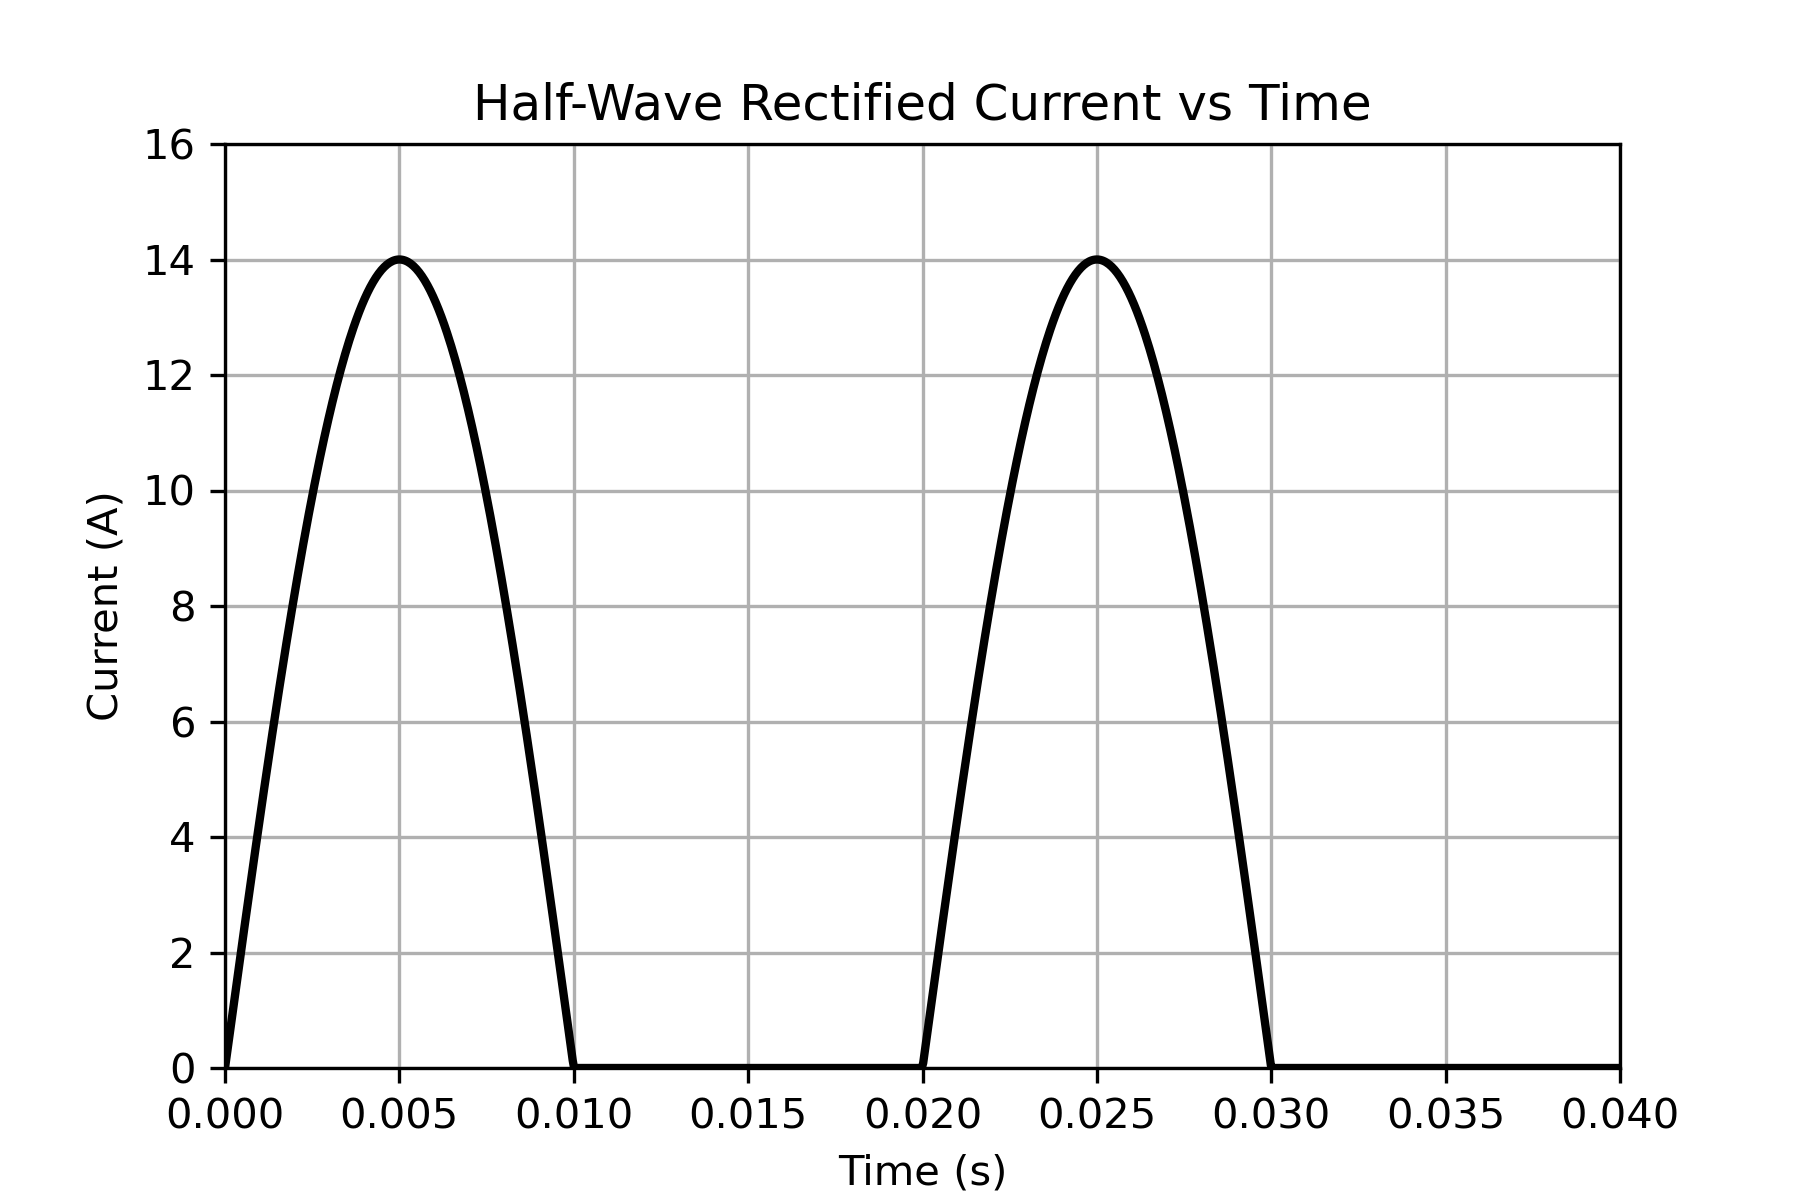
\includegraphics[width=0.8\columnwidth]{figs/half_wave_rectified.png}
  \caption{}
\end{figure}

(b) \begin{figure}[H]
  \centering
  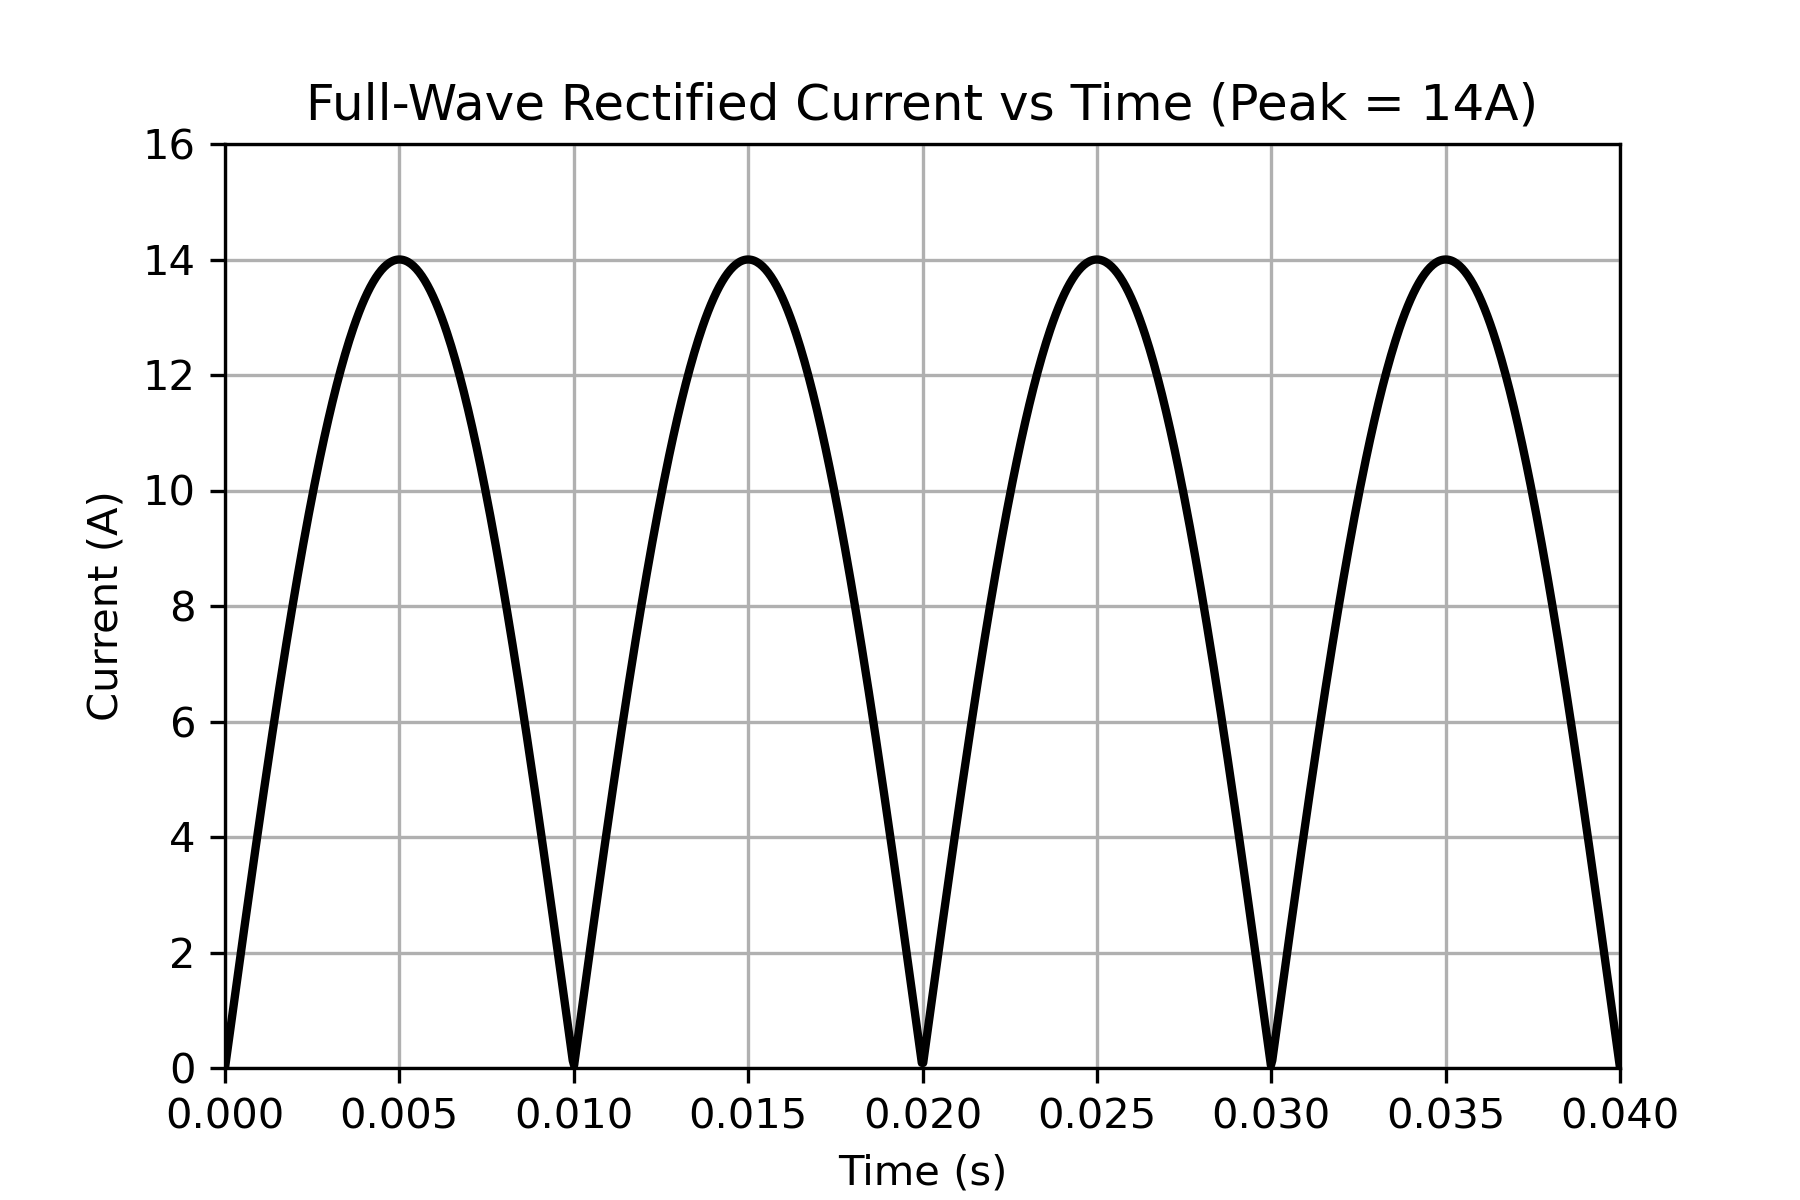
\includegraphics[width=0.8\columnwidth]{figs/full_wave_peak_14A.png}
  \caption{}
\end{figure}

(c) \begin{figure}[H]
  \centering
  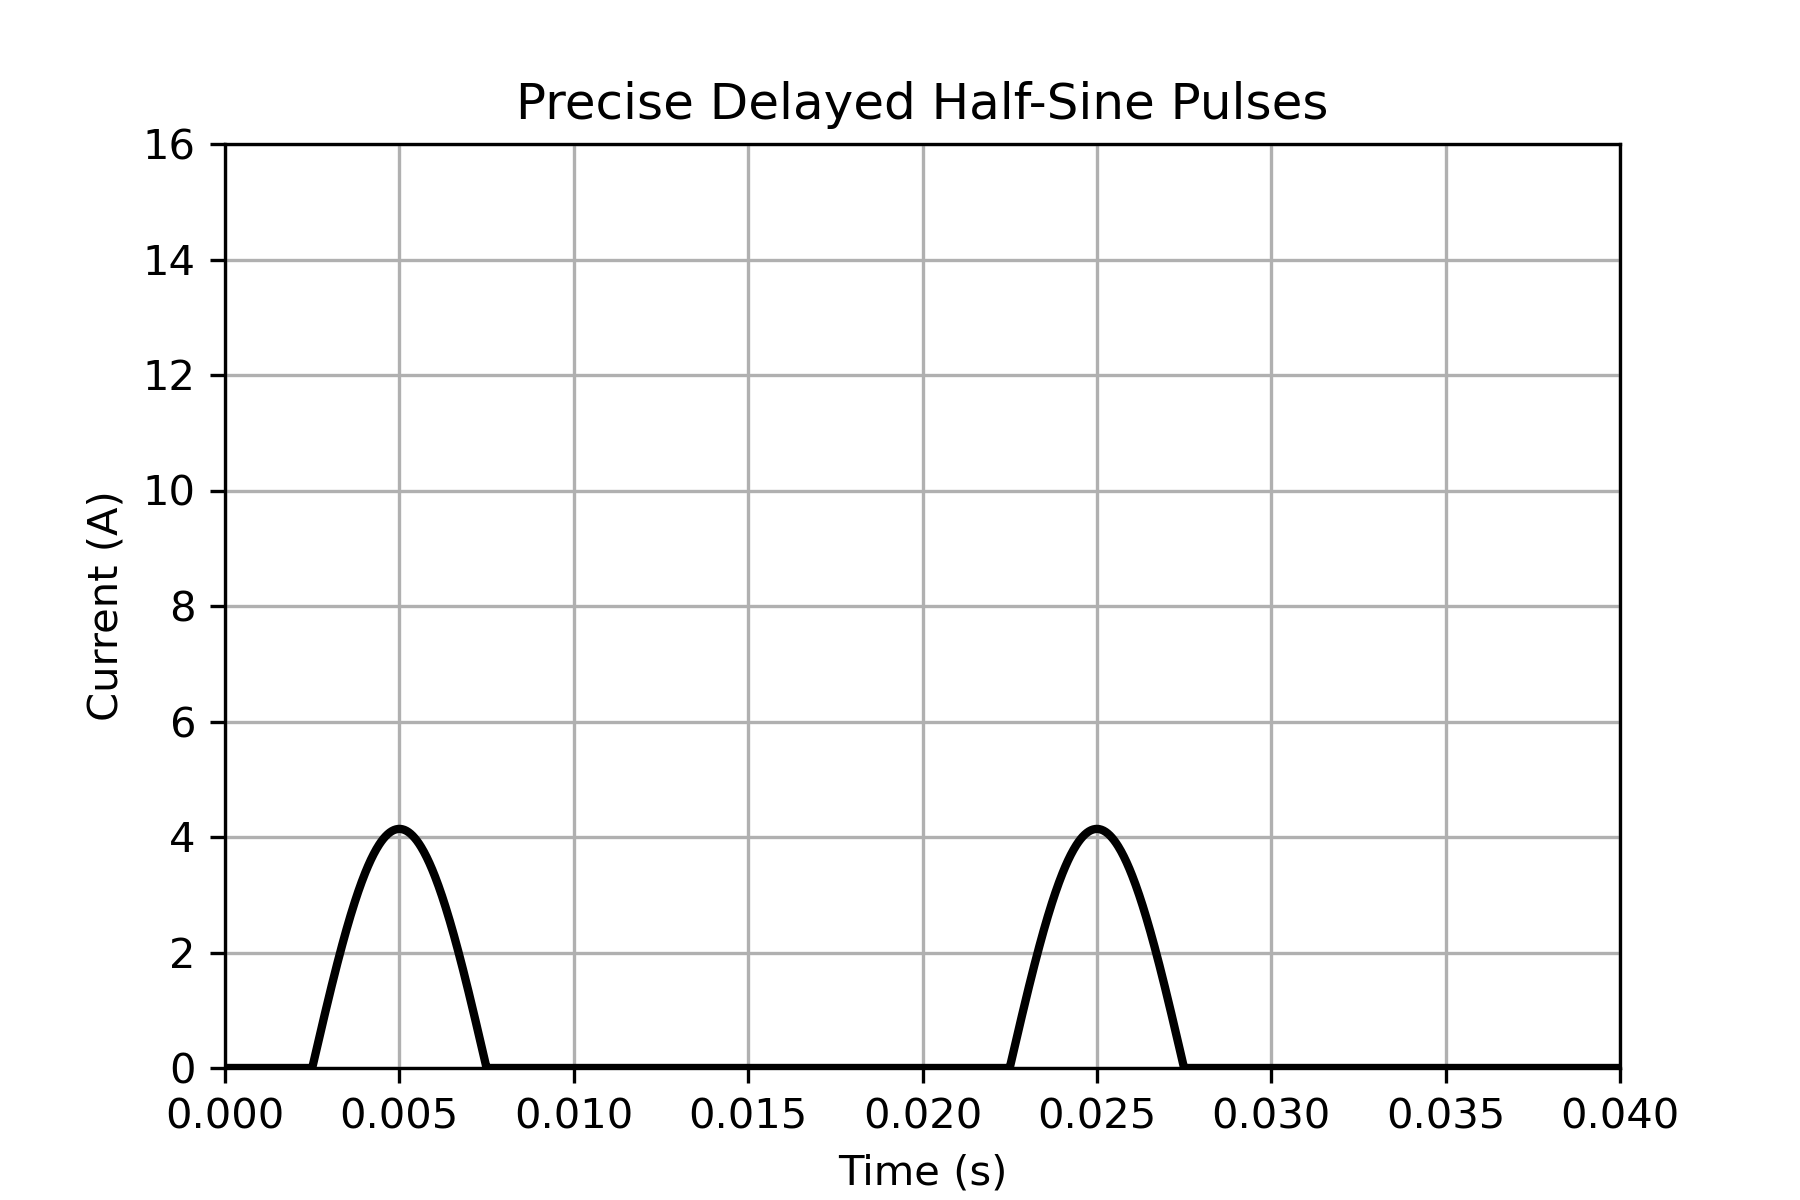
\includegraphics[width=0.8\columnwidth]{figs/precise_half_sine_pulses.png}
  \caption{}
\end{figure}

(d) \begin{figure}[H]
  \centering
  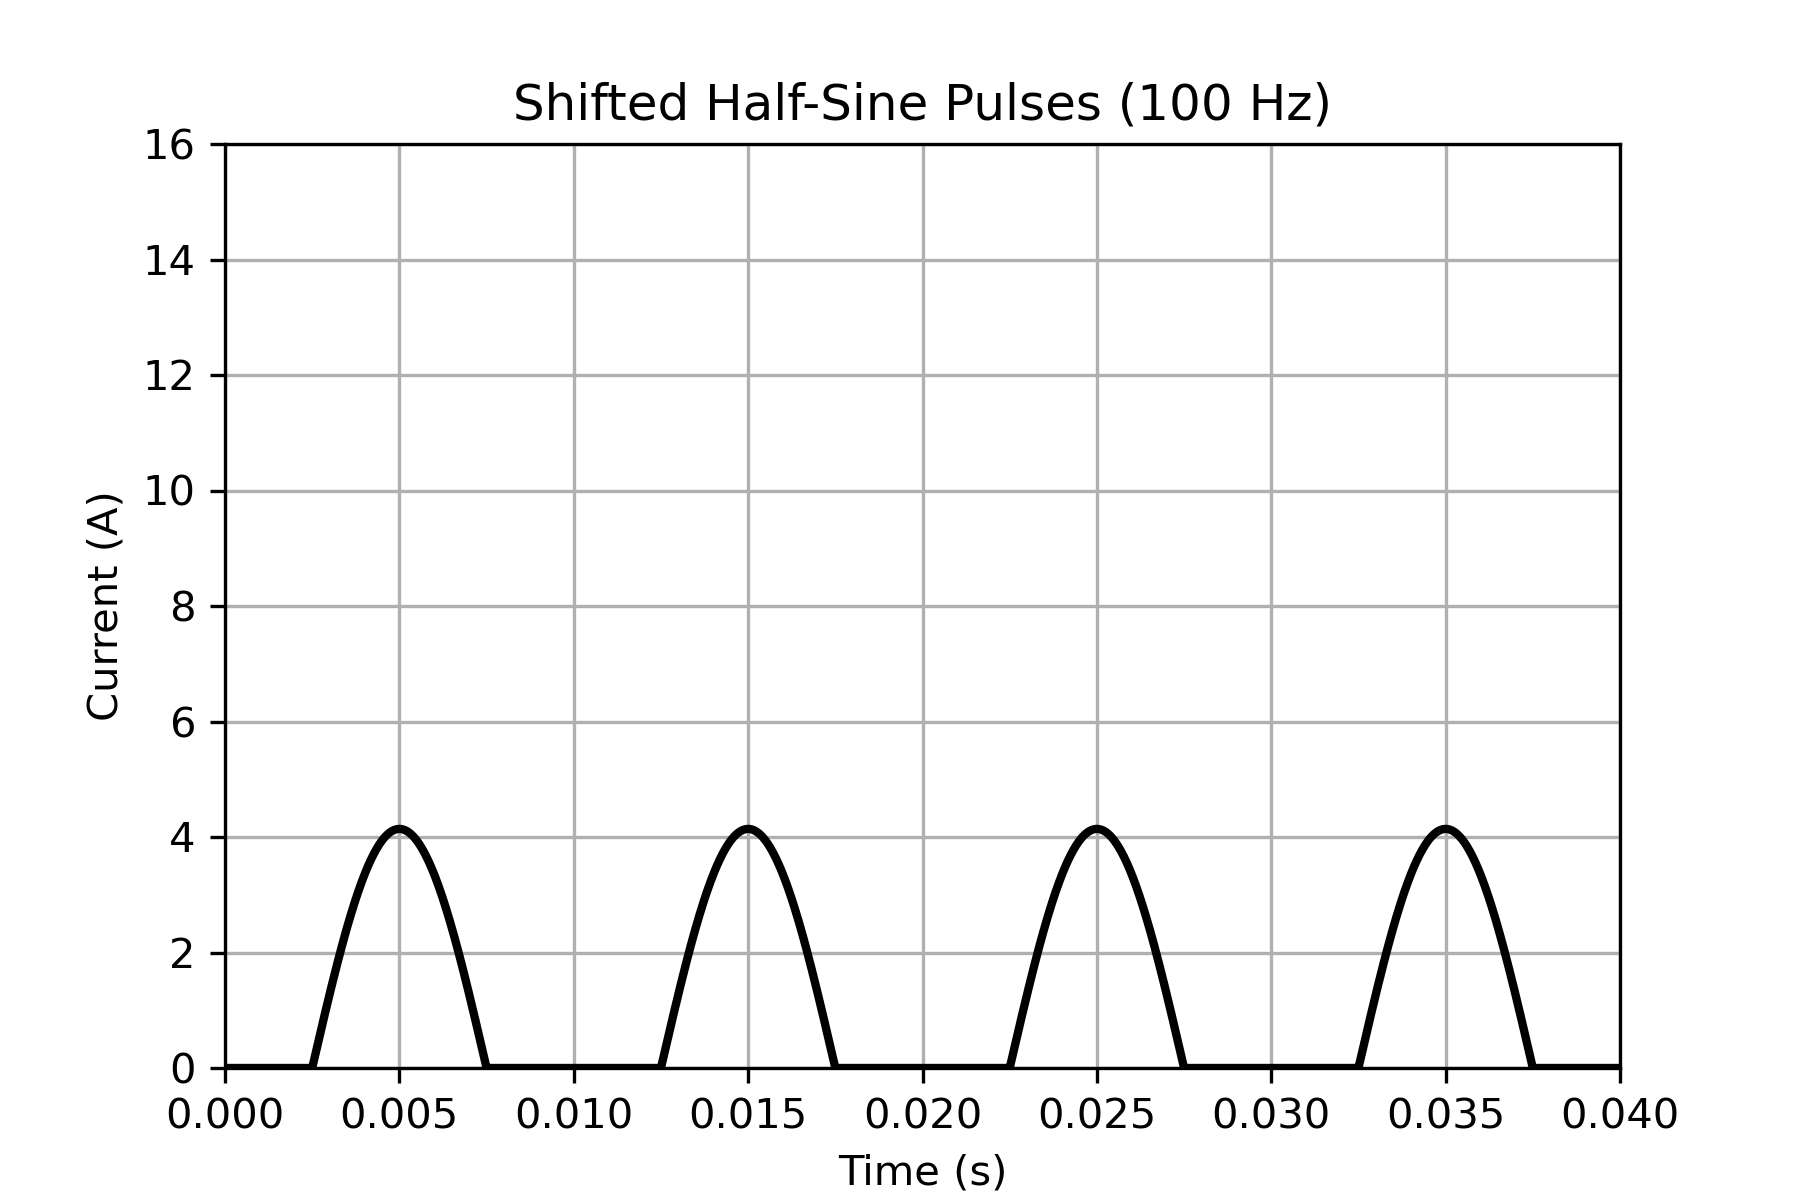
\includegraphics[width=0.8\columnwidth]{figs/shifted_half_sine_pulses.png}
  \caption{}
\end{figure}
\end{multicols}

(GATE XE 2008)
\item  For the counter shown in figure, the present count, $Q_{1}Q_{2}Q_{3}Q_{4}$ is $0100$. The count after two clock pulses will be

\begin{figure}[H]
\centering
\resizebox{0.9\columnwidth}{!}{%
\begin{circuitikz}
\tikzstyle{every node}=[font=\large]
\draw  (3.75,13.5) rectangle (6.5,10.25);
\draw  (7.75,13.5) rectangle (10.5,10.25);
\draw  (11.75,13.5) rectangle (14.5,10.25);
\draw  (15.75,13.5) rectangle (18.5,10.25);
\draw (3,12) to[short, -o] (3.75,12) ;
\draw (7.25,12) to[short, -o] (7.75,12) ;
\draw (11,12) to[short, -o] (11.75,12) ;
\draw (15.25,12) to[short, -o] (15.75,12) ;
\draw (3,12) to[short] (3,9.5);
\draw (7.25,12) to[short] (7.25,9.5);
\draw (11,12) to[short] (11,9.5);
\draw (15.25,12) to[short] (15.25,9.5);
\draw (1.25,9.5) to[short] (15.25,9.5);
\draw (3.75,13) to[short] (2.75,13);
\draw (2.75,13) to[short] (2.75,14.25);
\draw (2.75,14.25) to[short] (19.5,14.25);
\draw (19.5,14.25) to[short] (19.5,13);
\draw (19.5,13) to[short] (18.5,13);
\draw (15.75,13) to[short] (14.5,13);
\draw (11.75,13) to[short] (10.5,13);
\draw (7.75,13) to[short] (6.5,13);
\node [font=\LARGE] at (4,13) {$D_{1}$};
\node [font=\LARGE] at (6,13) {$Q_{1}$};
\node [font=\LARGE] at (6,10.5) {$Q_{1}$};
\node [font=\LARGE] at (8,13) {$D_{2}$};
\node [font=\LARGE] at (10,13) {$Q_{2}$};
\node [font=\LARGE] at (10,10.5) {$Q_{2}$};
\node [font=\LARGE] at (12.25,13) {$D_{3}$};
\node [font=\LARGE] at (14,13) {$Q_{3}$};
\node [font=\LARGE] at (14,10.5) {$Q_{3}$};
\node [font=\LARGE] at (16,13) {};
\node [font=\LARGE] at (18,13) {$Q_{4}$};
\node [font=\LARGE] at (18,10.5) {$Q_{4}$};
\node [font=\LARGE] at (6,11) {$$};
\draw (5.75,11) to[short] (6.25,11);
\draw (9.75,11) to[short] (10.25,11);
\draw (13.75,11) to[short] (14.25,11);
\node [font=\LARGE] at (16.25,13) {$D_{4}$};
\draw (17.75,11) to[short] (18.25,11);
\draw [short] (3.75,12.25) -- (4.25,12);
\draw [short] (3.75,11.75) -- (4.25,12);
\draw [short] (7.75,12.25) -- (8.25,12);
\draw [short] (7.75,11.75) -- (8.25,12);
\draw [short] (11.75,12.25) -- (12.25,12);
\draw [short] (11.75,11.75) -- (12.25,12);
\draw [short] (15.75,12.25) -- (16.25,12);
\draw [short] (15.75,11.75) -- (16.25,12);
\node [font=\large] at (5,13) {$SET$};
\node [font=\large] at (5,10.5) {$CLR$};
\node [font=\large] at (9,13) {$SET$};
\node [font=\large] at (9,10.5) {$CLR$};
\node [font=\large] at (13.25,13) {$SET$};
\node [font=\large] at (13,10.5) {$CLR$};
\node [font=\large] at (17,13) {$SET$};
\node [font=\large] at (17,10.5) {$CLR$};
\draw [short] (6.5,10.75) -- (7,10.75);
\draw [short] (10.5,10.75) -- (10.75,10.75);
\draw [short] (14.5,10.75) -- (15,10.75);
\draw [short] (18.5,10.75) -- (19,10.75);
\draw [short] (7,10.75) -- (7,10.5);
\draw [short] (10.75,10.75) -- (10.75,10.5);
\draw [short] (15,10.75) -- (15,10.5);
\node [font=\large] at (1,9.5) {$Clk$};
\end{circuitikz}
}%
\caption{}
\label{fig:my_label}
\end{figure}

\begin{enumerate}
\begin{multicols}{4}
\item  $0100$ 
\item  $0001$ 
\item  $0010$ 
\item  $1000$
\end{multicols}
\end{enumerate}

(GATE XE 2008)
\item[] \textbf{Q9 to Q30 carry two marks each}

\item  An incandescent lamp is rated for $200 V$, $100 W$. Neglect temperature effects. When the lamp consumes $121 W$, the supply voltage is

\begin{enumerate}
\begin{multicols}{4}
\item $242 V$ 
\item $220 V$ 
\item $180 V$ 
\item $165 V$
\end{multicols}
\end{enumerate}

(GATE XE 2008)

\item  In the circuit shown in the figure, the load resistance, $R_{1}$ draws $15$ A when it is $10\Omega$ and $20$ A when it is $5 \Omega$. The open circuit voltage across XY is

\begin{figure}[H]
\centering
\resizebox{0.5\columnwidth}{!}{%
\begin{circuitikz}
\tikzstyle{every node}=[font=\Large]
\draw  (4.25,14) rectangle (7.5,10.25);
\draw (7.5,13) to[short] (9.75,13);
\draw (7.5,11.25) to[short] (9.75,11.25);
\draw (9.75,13) to[R] (9.75,11.25);
\node at (8.75,13) [circ] {};
\node at (8.75,11.25) [circ] {};
\node [font=\Large] at (5.75,13.5) {$Resistive$};
\node [font=\Large] at (5.75,12.75) {$Circuit$};
\node [font=\Large] at (5.75,12) {$including$};
\node [font=\Large] at (5.75,11.25) {$Sources$};
\node [font=\Large] at (8.75,13.5) {$X$};
\node [font=\Large] at (8.75,10.75) {$Y$};
\draw [->, >=Stealth] (9.5,11.75) -- (10.25,12.5);
\node [font=\Large] at (10.5,12) {$R_{L}$};
\end{circuitikz}
}%
\caption{}
\label{fig:my_label}
\end{figure}

\begin{enumerate}
\begin{multicols}{4}
\item  $100 V$ 
\item  $150 V$ 
\item  $200 V$ 
\item  $300 V$
\end{multicols}
\end{enumerate}

(GATE XE 2008)
\item  Three $15$V batteries are connected to a resistive network as shown in the figure. The current in each resistor is

\begin{figure}[H]
\centering
\resizebox{0.5\columnwidth}{!}{%
\begin{circuitikz}
\tikzstyle{every node}=[font=\Large]
\draw (4,10.25) to[battery1] (4,11.75);
\draw (4,10.25) to[battery1] (5,9.25);
\draw (4,10.25) to[battery1] (2.75,9);
\draw (8.5,11.75) to[R] (8.5,10);
\draw (8.5,10) to[R] (9.75,8.75);
\draw (8.5,10) to[R] (7.25,8.75);
\draw (4,11.75) to[short] (8.5,11.75);
\draw (7.25,8.75) to[short] (5,8.75);
\draw (5,9.25) to[short] (5,8.75);
\draw (2.75,9) to[short] (2.75,8.25);
\draw (9.75,8.75) to[short] (9.75,8.25);
\draw (2.75,8.25) to[short] (9.75,8.25);
\node [font=\Large] at (4.75,11) {$15V$};
\node [font=\Large] at (3,10) {$15V$};
\node [font=\Large] at (5.25,10) {$15V$};
\node [font=\Large] at (7.75,11) {$10\Omega$};
\node [font=\Large] at (7.25,9.75) {$10\Omega$};
\node [font=\Large] at (9.75,9.75) {$10\Omega$};
\end{circuitikz}
}%
\caption{}
\label{fig:my_label}
\end{figure}

\begin{enumerate}
\begin{multicols}{4}
\item  $0.0A$ 
\item  $0.667A$ 
\item  $1.0A$ 
\item  $1.5A$
\end{multicols}
\end{enumerate}

(GATE XE 2008)
\item  At a particular frequency, the impedance across terminals AB in the figure shown is $(6.0 + j0.0)$ ohms. If $R_{1}= 12\Omega$, $C_{1} = 10\mu F$, $L_{1} = 0.2 H$, $R_{2} = 12\Omega$,$L_{2} = 0.1 H$, then $C_{2}$ is

\begin{figure}[H]
\centering
\resizebox{0.5\columnwidth}{!}{%
\begin{circuitikz}
\tikzstyle{every node}=[font=\Large]
\draw  (3.75,11.25) circle (0.75cm);
\draw (3.75,12) to[short] (3.75,13.75);
\draw (3.75,10.5) to[short] (3.75,8.25);
\draw (3.75,13.75) to[short] (8.5,13.75);
\draw (3.75,8.25) to[short] (8.5,8.25);
\draw (6.25,13.75) to[R] (6.25,12);
\draw (6.25,12) to[L ] (6.25,10);
\draw (6.25,10) to[C] (6.25,8.25);
\draw (8.5,13.75) to[R] (8.5,12);
\draw (8.5,12) to[L ] (8.5,10);
\draw (8.5,10) to[C] (8.5,8.25);
\node at (5.5,13.75) [circ] {};
\node at (5.5,8.25) [circ] {};
\node [font=\Large] at (3.75,11.25) {$AC$};
\node [font=\Large] at (5.5,13) {$R_{1}$};
\node [font=\Large] at (5.5,11) {$L_{1}$};
\node [font=\Large] at (5.5,9.25) {$C_{1}$};
\node [font=\Large] at (8,13) {$R_{2}$};
\node [font=\Large] at (8,11) {$L_{2}$};
\node [font=\Large] at (7.75,9.25) {$C_{2}$};
\node [font=\Large] at (5,14) {$A$};
\node [font=\Large] at (5,8) {$B$};
\end{circuitikz}
}%
\caption{}
\label{fig:my_label}
\end{figure}

\begin{enumerate}
\begin{multicols}{4}
\item $1.414 \mu F$ 
\item $5 \mu F$ 
\item $12 \mu F$ 
\item $20 \mu F$
\end{multicols}
\end{enumerate}

(GATE XE 2008)
\item  A transformer is feeding a $2.5$ kVA load at $0.8$ pf (lag). If its efficiency is $95\%$ and the copper losses equal $55$ W, the core loss is

\begin{enumerate}
\begin{multicols}{4}
\item  $25.13 W$ 
\item  $50.26 W$ 
\item  $100.54 W$ 
\item  $125.26 W$
\end{multicols}
\end{enumerate}

(GATE XE 2008)
\item The total winding resistance of a single-phase, two-winding transformer is half the magnitude of total impedance of the winding, both referred to the primary side. Considering the input and output voltages to be practically in-phase, the transformer will have zero regulation when the load power factor is

\begin{enumerate}
\begin{multicols}{4}
\item  $60^{\circ}$ lagging 
\item  $60^{\circ}$ leading 
\item  $30^{\circ}$ leading 
\item  $30^{\circ}$ lagging
\end{multicols}
\end{enumerate}

(GATE XE 2008)
\item A $220$ V dc shunt motor having an armature resistance, $r_{a}=0.5\Omega$ draws an armature current of $40$A when running at $1400$rpm. If the load torque is halved at the same field current and maintaining the same terminal voltage, then (neglecting armature reaction) the speed of the motor will be

\begin{enumerate}
\begin{multicols}{4}
\item  $1510$ rpm 
\item  $1485$ rpm 
\item  $1470$ rpm 
\item  $1370$ rpm
\end{multicols}
\end{enumerate}

(GATE XE 2008)
\item A $230$ V separately excited dc motor has armature resistance, $r_{a} = 2.0\Omega$. It draws $15$ A when running at a speed $N_{1}$. If the supply to the armature is disconnected, the field excitation and speed remaining unchanged, the voltage at the armature terminals will be

\begin{enumerate}
\begin{multicols}{4}
\item  $0 V$ 
\item  $200 V$ 
\item  $210 V$ 
\item  $240 V$
\end{multicols}
\end{enumerate}

(GATE XE 2008)
\item In an induction motor the phase-difference,$\phi$ between the voltage applied at the stator terminals and the magnetizing current is

\begin{enumerate}
\begin{multicols}{4}
\item  $\phi=0^{\circ}$
\item  $0^{\circ} < \phi <90^{\circ}$ 
\item  $\phi=90^{\circ}$ 
\item  $90^{\circ}<\phi < 180^{\circ}$ 
\end{multicols}
\end{enumerate}

(GATE XE 2008)
\item  A voltage of $+5$ V is applied (with respect to ground) to both the inputs $V_{1}$ and $V_{2}$ of an operational amplifier circuit shown in the figure. $R_{1} = 20 k\Omega$ and $R_{2} = 10 k\Omega$. The output voltage, $V_{o}$ is

\begin{figure}[H]
\centering
\resizebox{0.5\columnwidth}{!}{%
\begin{circuitikz}
\tikzstyle{every node}=[font=\Large]
\draw (3.25,12.5) to[R] (7.25,12.5);
\draw (3.25,11.5) to[R] (7.25,11.5);
\draw (6.75,12.5) to[short] (6.75,14);
\draw (6.75,14) to[R] (4.25,14);
\draw (4.25,14) to (4.25,13.75) node[ground]{};
\draw (6.75,11.5) to[short] (6.75,9.75);
\draw (6.75,9.75) to[R] (9.75,9.75);
\draw (9.75,9.75) to[short] (9.75,12);
\draw (8.5,11.5) to[short] (8.5,11);
\draw (8.5,12.5) to[short] (8.5,13);
\node at (3.25,12.5) [circ] {};
\node at (3.25,11.5) [circ] {};
\node at (10.25,12) [circ] {};
\node [font=\Large] at (2.75,12.5) {$V_{1}$};
\node [font=\Large] at (2.75,11.5) {$V_{2}$};
\node [font=\Large] at (5.5,14.5) {$R_{2}$};
\node [font=\Large] at (5.25,13) {$R_{1}$};
\node [font=\Large] at (5.25,11) {$R_{1}$};
\node [font=\Large] at (8.25,9.25) {$R_{2}$};
\node [font=\Large] at (10.75,12) {$V_{0}$};
\draw (8.75,12) node[op amp,scale=1, yscale=-1 ] (opamp2) {};
\draw (opamp2.+) to[short] (7.25,12.5);
\draw  (opamp2.-) to[short] (7.25,11.5);
\draw (9.95,12) to[short](10.25,12);
\end{circuitikz}
}%
\caption{}
\label{fig:my_label}
\end{figure}

\begin{enumerate}
\begin{multicols}{4}
\item  $-5V$ 
\item  $0V$ 
\item  $5V$ 
\item $20V$
\end{multicols}
\end{enumerate}

(GATE XE 2008)
\item A pair of zener diodes each with a drop of $0.7 V$ and a zener voltage of $4.7 V$ is connected as shown in the figure. The input voltage is $v_{in}=10\sin{(2t)}$. The peak-to-peak output voltage,$v_{o}$ is

\begin{figure}[H]
\centering
\resizebox{0.5\columnwidth}{!}{%
\begin{circuitikz}
\tikzstyle{every node}=[font=\Large]
\draw (0.5,13.75) to[sinusoidal voltage source, sources/symbol/rotate=auto] (0.5,10.5);
\draw (0.5,13.75) to[R] (4.25,13.75);
\draw (0.5,10.5) to[short] (4.25,10.5);
\draw (4.25,10.5) to[empty Zener diode] (4.25,13.75);
\draw (4.25,13.75) to[short] (6.25,13.75);
\draw (4.25,10.5) to[short] (6.25,10.5);
\draw (5.5,13.75) to[empty Zener diode] (5.5,10.5);
\node at (6.25,13.75) [circ] {};
\node at (6.25,10.5) [circ] {};
\node [font=\Large] at (-0.5,12.25) {$V_{in}$};
\node [font=\Large] at (7,12) {$V_{o}$};
\node [font=\Large] at (2.5,14.5) {$R_{s}$};
\end{circuitikz}
}%
\caption{}
\label{fig:my_label}
\end{figure}

\begin{enumerate}
\begin{multicols}{4}
\item  $5.4 V$ 
\item  $4.7 V$ 
\item  $1.4 V$ 
\item  $0.7 V$
\end{multicols}
\end{enumerate}

(GATE XE 2008)
\item  The npn transistor shown in figure has $h_{fe} = 99$ and $V_{BE} = 0.7 V$. Under quiescent condition, $V_{EG} =4.3 V$ and $I_{g} = 1 mA$, and the current in $R_{2}$ is $0.1 mA$. The value of $R$, required for biasing the circuit is

\begin{figure}[H]
\centering
\resizebox{0.5\columnwidth}{!}{%
\begin{circuitikz}
\tikzstyle{every node}=[font=\Large]
\draw (1,15.5) to[short] (4.75,15.5);
\draw (1,15.5) to[R] (1,11.75);
\draw (4.75,15.5) to[R] (4.75,13);
\draw (4.75,11) to[Tnpn, transistors/scale=1.19] (4.75,13);
\draw (4.75,11) to[R] (4.75,9.5);
\draw (1,11.75) to[R] (1,9.5);
\draw (1,9.5) to[short] (4.75,9.5);
\draw (2.75,15.5) to[short] (2.75,16);
\draw (2.75,9.5) to (2.75,8.75) node[ground]{};
\node at (2.75,16) [circ] {};
\draw (3.75,12) to[short] (1,12);
\node [font=\Large] at (3,16.5) {$15V$};
\node [font=\Large] at (5.25,14.25) {$R_{c}$};
\node [font=\Large] at (5.25,10.25) {$R_{E}$};
\node [font=\Large] at (0.25,10.5) {$R_{2}$};
\node [font=\Large] at (0.25,13.75) {$R_{1}$};
\node [font=\Large] at (3.75,12.25) {$B$};
\node [font=\Large] at (5,13) {$C$};
\node [font=\Large] at (4,11) {$I_{E}$};
\node [font=\Large] at (5,11.5) {$E$};
\node [font=\Large] at (3,9.25) {$G$};
\draw [->, >=Stealth] (4.25,11.25) -- (4.25,10.25);
\end{circuitikz}
}%
\caption{}
\label{fig:my_label}
\end{figure}

\begin{enumerate}
\begin{multicols}{4}
\item  $10.1 k\Omega$ 
\item  $90.9 k\Omega$ 
\item  $100.1 k\Omega$ 
\item  $150.2 k\Omega$
\end{multicols}
\end{enumerate}

(GATE XE 2008)
\item The forward characteristics of a p-n diode is given by $i =I_{s}e^{v/(nV_{T})}$ with $n = 2$ and $V_{T}= 25mV$. If the diode current is measured to be $100 mA$ at $0.7 V$ drop, the diode power dissipation at a diode current of $200 mA$ is

\begin{enumerate}
\begin{multicols}{4}
\item  $ 70 mW$ 
\item  $140 mW$ 
\item  $143 mW$ 
\item  $147 mW$
\end{multicols}
\end{enumerate}

(GATE XE 2008)
\item  For the n-channel JFET shown in the figure the pinch-off voltage, $V_{p} = -5 V$, and gate source voltage, $V_{GS} = -3 V$. The minimum required drain to source voltage, $V_{DS}$ to operate at pinch-off condition is

\begin{figure}[H]
\centering
\resizebox{0.5\columnwidth}{!}{%
\begin{circuitikz}
\tikzstyle{every node}=[font=\LARGE]
\draw  (1.5,14.75) rectangle (5.25,10.5);
\draw  (1.5,14.25) rectangle (2.5,11);
\draw  (5.25,14.25) rectangle (4.25,11);
\draw  (1.5,14) rectangle (1.25,11.25);
\draw  (5.25,14) rectangle (5.5,11.25);
\draw  (2,15) rectangle (4.75,14.75);
\draw  (2,10.5) rectangle (4.75,10.25);
\draw (3.25,10.25) to[short] (3.25,9.5);
\draw (1.25,13) to[short] (-1.25,13);
\draw (-1.25,9.5) to[battery1] (-1.25,13);
\draw (-1.25,9.5) to[crossing] (3.25,9.5);
\draw (1,13) to[short] (1,8.5);
\draw (1,8.5) to[short] (6.25,8.5);
\draw (6.25,8.5) to[short] (6.25,12.75);
\draw (6.25,12.75) to[short] (5.5,12.75);
\node at (1,13) [circ] {};
\draw (3.25,15) to[short] (3.25,16);
\node at (3.25,16) [circ] {};
\node at (3.25,9.5) [circ] {};
\node [font=\LARGE] at (3.25,16.5) {$V_{D}$};
\node [font=\LARGE] at (0.75,13.5) {$V_{S}$};
\node [font=\LARGE] at (3.75,9.25) {$V_{G}$};
\node [font=\LARGE] at (-1.25,11.75) {$V_{GS}$};
\node [font=\LARGE] at (3.25,14.5) {n};
\node [font=\LARGE] at (2,12.75) {p};
\node [font=\LARGE] at (4.75,12.75) {p};
\end{circuitikz}
}%
\caption{}
\label{fig:my_label}
\end{figure}

\begin{enumerate}
\begin{multicols}{4}
\item  $0V$ 
\item  $2 V$ 
\item  $5V$ 
\item  $8 V$
\end{multicols}
\end{enumerate}

(GATE XE 2008)
\item  The Boolean function corresponding to the truth table shown is

\begin{table}[H]     \centering     \caption{}     \label{}     \begin{tabular}{c|c|c|c}
    A & B & C & \textbf{F}  \\
    \hline
    0 & 0 & 0 & \textbf{1}   \\
    \hline
    0 & 0 & 1 & \textbf{1}  \\
    \hline
    0 & 1 & 0 & \textbf{0} \\
    \hline
    0 & 1 & 1 & \textbf{1} \\
    \hline
    1 & 0 & 0 & \textbf{0} \\
    \hline
    1 & 0 & 1 & \textbf{1} \\
    \hline
    1 & 1 & 0 & \textbf{0} \\
    \hline
    1 & 1 & 1 & \textbf{0} \\
    \hline
\end{tabular} \end{table}

\begin{enumerate}
\item  $F=A\bar{B}C + \bar{A}BC +\bar{A}\bar{B}C + \bar{A}\bar{B}\bar{C}$
\item  $F=ABC + AB\bar{C} + \bar{A}BC$
\item  $F=ABC + AB\bar{C} +A\bar{B}\bar{C} +\bar{A}B\bar{C}$
\item  $F=A\bar{B}C + \bar{A}BC + \bar{A}\bar{B}C + \bar{A}BC$
\end{enumerate}

(GATE XE 2008)
\item  The decimal number $328$ when converted to the base of $9$ is equivalent to

\begin{enumerate}
\begin{multicols}{4}
\item  $(434)_{9}$ 
\item  $(424)_{9}$ 
\item  $(404)_{9}$ 
\item  $(304)_{9}$
\end{multicols}
\end{enumerate}

(GATE XE 2008)
\item  The following logic circuit can be represented by the Boolean expression

\begin{figure}[H]
\centering
\resizebox{0.8\columnwidth}{!}{%
\begin{circuitikz}
\tikzstyle{every node}=[font=\LARGE]
\draw (0.75,15.75) to[short] (1,15.75);
\draw (0.75,15.25) to[short] (1,15.25);
\draw (1,15.75) node[ieeestd nor port, anchor=in 1, scale=0.89](port){} (port.out) to[short] (2.75,15.5);
\draw (4.5,15.5) to[short] (4.75,15.5);
\draw (4.5,15) to[short] (4.75,15);
\draw (4.75,15.5) node[ieeestd xnor port, anchor=in 1, scale=0.89](port){} (port.out) to[short] (6.5,15.25);
\draw (4.75,12.75) node[ieeestd not port, anchor=in](port){} (port.out) to[short] (6.5,12.75);
\draw (port.in) to[short] (4.5,12.75);
\draw (0.75,13) to[short] (1,13);
\draw (0.75,12.5) to[short] (1,12.5);
\draw (1,13) node[ieeestd and port, anchor=in 1, scale=0.89](port){} (port.out) to[short] (2.75,12.75);
\draw (7.5,14.25) to[short] (7.75,14.25);
\draw (7.5,13.75) to[short] (7.75,13.75);
\draw (7.75,14.25) node[ieeestd or port, anchor=in 1, scale=0.89](port){} (port.out) to[short] (9.5,14);
\draw (0.75,15.75) to[short] (-1.25,15.75);
\draw (0.75,15.25) to[short] (-1.25,15.25);
\draw (-0.25,15.25) to[short] (-0.25,13);
\draw (-0.25,13) to[short] (0.75,13);
\draw (0.75,12.5) to[short] (-1.25,12.5);
\draw (2.75,12.75) to[short] (4.75,12.75);
\draw (2.75,15.5) to[short] (4.5,15.5);
\draw (3.5,12.75) to[short] (3.5,15);
\draw (3.5,15) to[short] (4.5,15);
\draw (6.5,15.25) to[short] (7,15.25);
\draw (7,15.25) to[short] (7,14.25);
\draw (7,14.25) to[short] (7.5,14.25);
\draw (6.5,12.75) to[short] (7,12.75);
\draw (7,12.75) to[short] (7,13.75);
\draw (7,13.75) to[short] (7.75,13.75);
\node [font=\LARGE] at (-1.5,16) {A};
\node [font=\LARGE] at (-1.5,15.25) {B};
\node [font=\LARGE] at (-1.5,12.5) {C};
\node [font=\LARGE] at (9.75,14) {F};
\end{circuitikz}
}%
\caption{}
\label{fig:my_label}
\end{figure}

\begin{enumerate}
\begin{multicols}{2}
\item  $F=\bar{B} + BC + \bar{C}$
\item  $F=\bar{B} + \bar{C}$
\item  $F=\overline{(B+C)}$
\item  $F=\bar{A} + \bar{B} +\bar{C}$
\end{multicols}
\end{enumerate}

(GATE XE 2008)
\item A 4-bit resistor network based D/A converter is shown in the figure. The output corresponding to
the number $1010$ is

\begin{figure}[H]
\centering
\resizebox{0.8\columnwidth}{!}{%
\begin{circuitikz}
\tikzstyle{every node}=[font=\LARGE]
\draw (-0.5,16.5) to[battery1] (-0.5,13.25);
\draw (-0.5,13.25) to (-0.5,11.75) node[ground]{};
\draw (1.25,16.5) to[normal open switch] (1.25,14.25);
\draw (2.75,16.5) to[normal open switch] (2.75,14.25);
\draw (4.25,16.5) to[normal open switch] (4.25,14.25);
\draw (5.5,16.5) to[normal open switch] (5.5,14.25);
\draw (-0.5,16.5) to[short] (5.5,16.5);
\draw (1.25,14.25) to[R] (1.25,12.25);
\draw (2.75,14.25) to[R] (2.75,12.25);
\draw (4.25,14.25) to[R] (4.25,12.25);
\draw (5.5,14.25) to[R] (5.5,12.25);
\draw (1.25,12.25) to[short] (6.5,12.25);


\draw (7.75,11.75) node[op amp,scale=1] (opamp2) {};
\draw (opamp2.+) to[short] (6.25,11.25);
\draw  (opamp2.-) to[short] (6.25,12.25);
\draw (8.95,11.75) to[short](9.25,11.75);
\draw (6.25,11.25) to (6.25,10.25) node[ground]{};
\draw (6.25,12.25) to[short] (6.25,13.75);
\draw (6.25,13.75) to[R] (8.5,13.75);
\draw (8.5,13.75) to[short] (8.5,11.75);
\node at (9.25,11.75) [circ] {};
\draw (7.5,12.25) to[short] (7.5,12.75);
\draw (7.5,11.25) to[short] (7.5,10.75);
\node [font=\large] at (0,15.25) {-10V};
\node [font=\LARGE] at (1,16.75) {MSB};
\node [font=\LARGE] at (5.5,16.75) {LSB};
\node [font=\large] at (1.75,13.25) {10k};
\node [font=\large] at (3.5,13.25) {20k};
\node [font=\large] at (4.75,13.25) {40k};
\node [font=\large] at (6,13.25) {80k};
\node [font=\large] at (7.25,14.25) {5k};
\node [font=\LARGE] at (9.75,11.75) {$V_{o}$};
\node [font=\large] at (1,15.25) {1};
\node [font=\large] at (1.75,15.25) {0};
\node [font=\large] at (2.5,15.25) {1};
\node [font=\large] at (3.25,15.25) {0};
\node [font=\large] at (4,15.25) {1};
\node [font=\large] at (4.75,15.25) {0};
\node [font=\large] at (5.25,15.25) {1};
\node [font=\large] at (6,15.25) {0};
\end{circuitikz}
}%
\caption{}
\label{fig:my_label}
\end{figure}

\begin{enumerate}
\begin{multicols}{4}
\item  $5.0 V$ 
\item  $6.25 V$ 
\item  $7.25 V$ 
\item  $10.0 V$
\end{multicols}
\end{enumerate}

(GATE XE 2008)
\item  Two $10 V$ square waves of same frequency but $90^{\circ}$ out-of-phase to each other are applied to X and Y deflecting plates of a CRO. Both channels are set at $5 V$/division and the CRO is operating in the X-Y mode. The display on CRO will be

\begin{enumerate}

\item  A bright circle

\item  A bright ellipse

\item  Two bright spots at the diagonal of a faint square

\item  Four bright spots at the corners of a faint square
\end{enumerate}

(GATE XE 2008)
\item  A CRO that is used in X-Y mode displays a line inclined at an angle of $135^{\circ}$. The X-channel gain is $5V$/division and the Y-channel gain is $10V$/division. If the display point at a given instant corresponds to $+ 3$ divisions on the X-axis, the input voltage to the Y-channel at that instant is

\begin{enumerate}
\begin{multicols}{4}
\item  $-30 V$ 
\item  $-15 V$
\item  $+15 V$ 
\item  $+30 V$
\end{multicols}
\end{enumerate}

(GATE XE 2008)
\item[]\textbf{\Large Common Data Questions}

\textbf{Common Data for Questions 29 and 30}

A $1.0 kW$ induction motor has $15$ pole-pairs and is supplied from a $60 Hz$ source. The motor runs at $0.05$ slip. The stator loss is $80 W$.

\item  The speed of the rotating magnetic field in the motor and the frequency of the rotor induced voltage are

\begin{enumerate}
\begin{multicols}{2}
\item  $120 rpm , 1.5 Hz$
\item  $120 rpm, 28.5 Hz$
\item  $240 rpm, 3.0 Hz$
\item  $240 rpm, 57.0 Hz$
\end{multicols}
\end{enumerate}

(GATE XE 2008)
\item  The rotor copper loss of this induction motor is

\begin{enumerate}
\begin{multicols}{4}
\item  $4.6 W$ 
\item  $42 W$ 
\item  $46 W$  
\item  $54 W$
\end{multicols}
\end{enumerate}

(GATE XE 2008)
\item[]\textbf{\Large Linked Answer Questions: Q.31 to Q.34 carry two marks each.}

\textbf{Statement for Linked Answer Questions 31 and 32:}

A practical de voltage source is represented as an ideal dc voltage source in series with an internal
resistance. The V-I characteristics of two such sources, $E_{1}$ and $E_{2}$, are shown in the figure.

\begin{figure}[H]
  \centering
  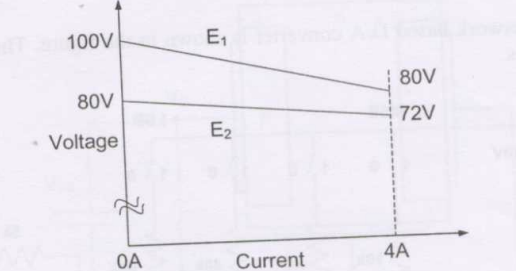
\includegraphics[width=0.8\columnwidth]{figs/q31.png}
  \caption{}
\end{figure}

\item  The respective internal resistances of $E_{1}$ and $E_{2}$ are

\begin{enumerate}
\begin{multicols}{4}
\item  $20 \Omega, 8 \Omega$ 
\item  $5 \Omega, 2 \Omega$ 
\item  $8\Omega, 20\Omega$ 
\item  $2 \Omega, 5\Omega$
\end{multicols}
\end{enumerate}

(GATE XE 2008)
\item  If the two sources, $E_{1}$ and $E_{2}$, in question Q.31 are connected in parallel to feed a load of $200\Omega$ resistance, then the load current is in the range

\begin{enumerate}
\begin{multicols}{2}
\item  $0.0 A$ to $0.5 A$
\item  $0.5 A$ to $2.0 A$
\item  $2.0 A$ to $4.0 A$
\item  $4.0 A$ to $8.0 A$
\end{multicols}
\end{enumerate}

(GATE XE 2008)
\item[] \textbf{Statement for Linked Answer Questions 33 and 34:}

A function F, in "Sum of Product (SOP)" form is described by$ F = \sum m (0,1,3,4,5,6,7,13,15)$

\item  The Karnaugh Map for F is given by (X being don't care)

\begin{enumerate}
\begin{multicols}{2}
\item 

\begin{center}
\renewcommand{\arraystretch}{1.4}
\begin{table}[H]     \centering     \caption{}     \label{}     \begin{tabular}{|c|c|c|c|c|}
\hline
\multirow{2}{*}{AB $\backslash$ CD} & 00 & 01 & 11 & 10 \\
\cline{2-5}
& & & & \\
\hline
00 & X & X & X & 1 \\
\hline
01 & X & X & X & X \\
\hline
11 & 1 & X & X & 1 \\
\hline
10 & 1 & 1 & 1 & 1 \\
\hline
\end{tabular} \end{table}
\end{center}

\item  \begin{center}
\renewcommand{\arraystretch}{1.4}
\begin{table}[H]     \centering     \caption{}     \label{}     \begin{tabular}{|c|c|c|c|c|}
\hline
\multirow{2}{*}{AB $\backslash$ CD} & 00 & 01 & 11 & 10 \\
\cline{2-5}
& & & & \\
\hline
00 & 1 & 1 & 1 & X \\
\hline
01 & 1 & 1 & 1 & 1 \\
\hline
11 & X & 1 & 1 & X \\
\hline
10 & X & X & X & X \\
\hline
\end{tabular} \end{table}
\end{center}

\item  \begin{center}
\renewcommand{\arraystretch}{1.4}
\begin{table}[H]     \centering     \caption{}     \label{}     \begin{tabular}{|c|c|c|c|c|}
\hline
\multirow{2}{*}{AB $\backslash$ CD} & 00 & 01 & 11 & 10 \\
\cline{2-5}
& & & & \\
\hline
00 & 1 & X & 1 & X \\
\hline
01 & X & 1 & X & 1 \\
\hline
11 & 1 & X & X & X \\
\hline
10 & X & 1 & X & 1 \\
\hline
\end{tabular} \end{table}
\end{center}

\item  \begin{center}
\renewcommand{\arraystretch}{1.4}
\begin{table}[H]     \centering     \caption{}     \label{}     \begin{tabular}{|c|c|c|c|c|}
\hline
\multirow{2}{*}{AB $\backslash$ CD} & 00 & 01 & 11 & 10 \\
\cline{2-5}
& & & & \\
\hline
00 & 1 & 1 & X & X \\
\hline
01 & X & X & X & X \\
\hline
11 & X & 1 & 1 & 1 \\
\hline
10 & X & 1 & 1 & X \\
\hline
\end{tabular} \end{table}
\end{center}

\end{multicols}
\end{enumerate}

(GATE XE 2008)

\item  Using the Karnaugh Map obtained in question Q.33, the function, F reduces to

\begin{enumerate}
\begin{multicols}{2}
\item  $F =\bar{A}\bar{C} + \bar{A}D + AB + BD$
\item  $F = AC+ AD + \bar{A}\bar{B}+\bar{B}\bar{D}$
\item  $F = AC + \bar{A}D + \bar{A}\bar{B}+\bar{B}\bar{D}$
\item  $F = \bar{A}\bar{C}+ \bar{A}D+\bar{A}B+BD$
\end{multicols}
\end{enumerate}

(GATE XE 2008)

\begin{center}
    \textbf{END OF SECTION-C}
\end{center}


\end{enumerate}
\newpage
\begin{center}
    \textbf{D : FLUID MECHANICS}
\end{center}

 \textbf{\underline{Useful data:}}
 \begin{center}
     Acceleration due to gravity, $g =10 m/s^{2}$\\
Density of water $\rho _{w} = 1000 kg/m^{3}$\\
Density of air (unless otherwise specified),$ \rho _{o}=1.2kg/m^{3}$
 \end{center}

\begin{enumerate}
\item[] \textbf{Q1 - Q8 carry one mark each}

\item A potential function can be defined for a flow if and only if it is

\begin{enumerate}
\begin{multicols}{4}
\item  laminar  
\item  incompressible  
\item  steady  
\item  irrotational
\end{multicols}
\end{enumerate}


(GATE XE 2008)
\item The momentum equation (Euler),\\
$\frac{\partial u}{\partial t}+ u \frac{\partial u}{\partial x}+v\frac{\partial u}{\partial y}+w\frac{\partial u}{\partial z} = -\frac{1}{\rho} \frac{\partial p}{\partial x}$ ,\\
is valid if and only if the flow is

\begin{enumerate}
\begin{multicols}{4}
\item  unsteady 
\item  laminar 
\item  steady 
\item  inviscid
\end{multicols}
\end{enumerate}

(GATE XE 2008)
\item Which of the following statements is true for two kinematically similar flows?

\begin{enumerate}
\item  They must be geometrically similar but may or may not be dynamically similar

\item  They must be dynamically similar but may or may not be geometrically similar

\item  They must be neither geometrically similar nor dynamically similar

\item  They must be both geometrically similar and dynamically similar
\end{enumerate}

(GATE XE 2008)
\item  The Darcy-Weisbach equation for head loss is valid

\begin{enumerate}
\item  only for laminar flow through smooth pipes

\item  only for turbulent flow through rough pipes

\item  for laminar or turbulent flows through smooth pipes only

\item  for laminar or turbulent flow through smooth or rough pipes
\end{enumerate}

(GATE XE 2008)
\item A ceiling fan of diameter, $D$, and weight, $W$, is suspended at a distance, $L$, below the ceiling by a support rod. When the fan spins at high speed and creates a downward flow the force exerted by the fan on the support rod is

\begin{enumerate}
\begin{multicols}{2}
\item  greater than $W$
\item  less than $W$
\item  equal to $W$
\item  greater than or less than $W$ depending on the value of $D/L$
\end{multicols}
\end{enumerate}

(GATE XE 2008)
\item Logs of the following cross-section are fully submerged horizontally in water


    
\begin{figure}[H]
\centering
  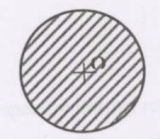
\includegraphics[width=0.2\columnwidth]{figs/ass1_d_q6_1.png}
  \caption{Solid Cylinder}
\end{figure} 
\begin{figure}[H]
\centering
  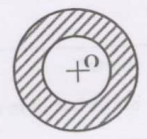
\includegraphics[width=0.2\columnwidth]{figs/ass1_d_q6_2.png}
  \caption{Hollow Cylinder}
  \end{figure} 
\begin{figure}[H]
\centering
  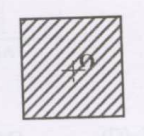
\includegraphics[width=0.2\columnwidth]{figs/ass1_d_q6_3.png}
  \caption{Solid Square}
  \end{figure} 
\begin{figure}[H]
  \centering
  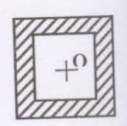
\includegraphics[width=0.2\columnwidth]{figs/ass1_d_q6_4.png}
  \caption{Hollow square}
\end{figure}

The buoyancy force passes through the point 'O' for which of the following cross-sections?

\begin{enumerate}
\begin{multicols}{2}
\item  Solid cylinder only 
\item  Solid cylinder and hollow cylinder \newline only 
\item  All the cross sections except hollow square 
\item  All the cross sections
\end{multicols}
\end{enumerate}

(GATE XE 2008)
\item A fluid particle can accelerate

\begin{enumerate}
\item  in a steady non-uniform flow-field
\item  only if the flow field is both unsteady and non-uniform 
\item  only in an unsteady flow-field
\item  in a steady uniform flow-field if the viscous forces are large enough
\end{enumerate}

(GATE XE 2008)
\item A fluid element is said to have vorticity with respect to a reference frame if in that reference frame

\begin{enumerate}
\item  it travels along a circular streamline
\item  it travels along a circular pathline
\item  it revolves about any arbitrary point in the flow-field
\item  it rotates about its own centre of mass as it moves
\end{enumerate}

(GATE XE 2008)
\item[] \textbf{Q. 9 to Q.30 carry two marks each.}

\item A cubical block of melting ice ($20 cm x 20 cm x 20 cm$) rests on a smooth horizontal floor over a layer of water of $0.1 mm$ thickness. To pull the block at a speed of $1 m/s$ a force of $1 N$ is required. What is the force required to pull the block at a speed of $2 m/s$?

\begin{enumerate}
\begin{multicols}{4}
\item  $0.5 N$ 
\item  $1 N$ 
\item  $2 N$ 
\item  $4 N$
\end{multicols}
\end{enumerate}

(GATE XE 2008)
\item  Which of the following statements is true?

\begin{enumerate}
\item  Eulerian description of fluid motion follows individual fluid particles 
\item  Lagrangian description of fluid motion is a field description 
\item  Both Eulerian and Lagrangian descriptions follow individual fluid particles but in different reference frames
\item  Eulerian description is a field description while Lagrangian description follows individual fluid particles
\end{enumerate}

(GATE XE 2008)
\item The velocity in a wind tunnel is being measured using a Pitot-static tube connected to a vertical U- tube manometer. The density of air is $1.2 kg/m^3$ and the deflection of the manometer is $24 mm$. The manometric fluid is water. The velocity measured by the Pitot-static tube is:

\begin{enumerate}
\begin{multicols}{4}
\item  $14.1 m/s$ 
\item  $20.0 m/s$ 
\item  $22.0 m/s$ 
\item  $400 m/s$
\end{multicols}
\end{enumerate}


(GATE XE 2008)
\item  The stream function for a potential flow around a corner is given by $y(x, y) = kxy$, where $k$ is a constant. The slopes of the streamline and the potential line passing through the point $(1,1)$ are respectively

\begin{figure}[H]
\centering
  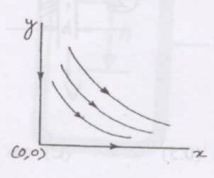
\includegraphics[width=0.3\columnwidth]{figs/ass1_d_q12.png}
  \caption{}
\end{figure} 

\begin{enumerate}
\begin{multicols}{4}
\item  1 and-1 
\item  -1 and 
\item  1 and 1 
\item  -1 and-1
\end{multicols}
\end{enumerate}

(GATE XE 2008)
\item The non-dimensional numbers shown in column 1 relate the inertial force with another force shown in column 2. Match the dimensionless number with the corresponding force.

\begin{table}[H]     \centering     \caption{}     \label{}     \begin{tabular}{l   l}
    Column 1 & Column 2 \\
      &  \\
   R: Reynolds number & P: Pressure\\
F: Froude number & G: Gravity\\
E: Euler number & S: Surface tension\\
W: Weber number & V: Viscous\\
\end{tabular} \end{table}

\begin{enumerate}
\begin{multicols}{2}
\item  R-G, F-P, E-S, W-V
\item  R-V, F-G, E-S, W-P
\item  R-G, F-V, E-S, W-P
\item  R-V, F-G, E-P, W-S
\end{multicols} 
\end{enumerate}


(GATE XE 2008)
\item  Consider the aerofoil of the dimensions shown. The lift coefficient Ct is measured to be $1.4$ (based on the largest projected area). If air of density $1.2 kg/m^3$ flows over the aerofoil at $50 m/s$ the lift force is:

\begin{figure}[H]
\centering
  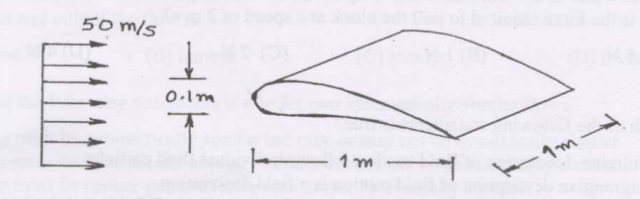
\includegraphics[width=0.5\columnwidth]{figs/ass1_d_q14.png}
  \caption{}
\end{figure} 

\begin{enumerate}
\begin{multicols}{4}
\item  $2.1 kN$ 
\item  $1.5 kN$ 
\item  $0.21 kN$ 
\item  $0.042 kN$
\end{multicols}
\end{enumerate}

(GATE XE 2008)
\item A two-dimensional water jet hits a splitter plate as shown. The velocities at sections 1,2 and 3 may be taken as uniform and equal to $V$. The weight of the water and the friction along the plate may be neglected. For the data shown what is $\theta$?

\begin{figure}[H]
\centering
  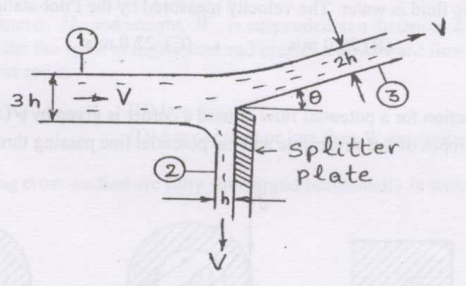
\includegraphics[width=0.5\columnwidth]{figs/ass1_d_q15.png}
  \caption{}
\end{figure} 

\begin{enumerate}
\begin{multicols}{4}
\item  $0$ 
\item  $\tan^{-1} (0.5)$ 
\item  $\cos^{-1}(0.5)$ 
\item  $\sin^{-1}(0.5)$
\end{multicols}
\end{enumerate}

(GATE XE 2008)
\item Find the vertical hydrostatic force, $f_{z}$, on the surface P-Q due to the water in the tank. Note, $f_{z}$ is the force per unit width along $y$. The surface P-Q is shaped like a quarter-cylinder of radius $R$.. The atmospheric pressure is $P_{o}$.

\begin{figure}[H]
\centering
  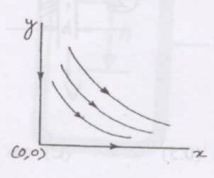
\includegraphics[width=0.5\columnwidth]{figs/ass1_d_q12.png}
  \caption{}
\end{figure} 

\begin{enumerate}
\begin{multicols}{2}
\item  $\rho _{w} (R^2 +\frac{\pi}{4}R^2)$
\item  $P_{o} R + \rho _{w} g (R^2 +\frac{\pi}{4}R^2)$
\item  $\rho _{w} g (\frac{\pi}{4} R^2)$
\item  $P_{o} R + \rho _{w} g (\frac{\pi}{4} R^2)$
\end{multicols}
\end{enumerate}

(GATE XE 2008)
\item For a given location in a flow, the rate of change of density following a fluid particle
$(\frac{D\rho}{Dt} = \frac{\partial \rho}{\partial t} + u\frac{\partial \rho}{\partial x} + v\frac{\partial \rho}{\partial y} + w\frac{\partial \rho}{\partial z})$, is $2.4 kg/(m^3 s)$.I the denst at that poin is $1.2 kg/m^3$, then
the divergence of the velocity field $(\nabla \cdot \vec{V})$ at that point is:

\begin{enumerate}
\begin{multicols}{4}
\item  $0.5 s^{-1}$ 
\item  $-0.5 s^{-1}$ 
\item  $-2 s^{-1}$ 
\item  $2 s^{-1}$
\end{multicols}
\end{enumerate}

(GATE XE 2008)
\item Water is flowing with volume flow rate $Q$ through a pipe whose diameter reduces to half across a reducer. If the flow is frictionless, compare the manometer reading $h_1$,$h_2$ and $h_3$, corresponding to the three different inclinations of the pipe $\theta _1 = 30^{\circ}$, $\theta _2 = 0^{\circ}$and $\theta _3 =-30^{\circ}$. Note that only the pipe tilts, while the manometer always stays vertical.

\begin{figure}[H]
\centering
  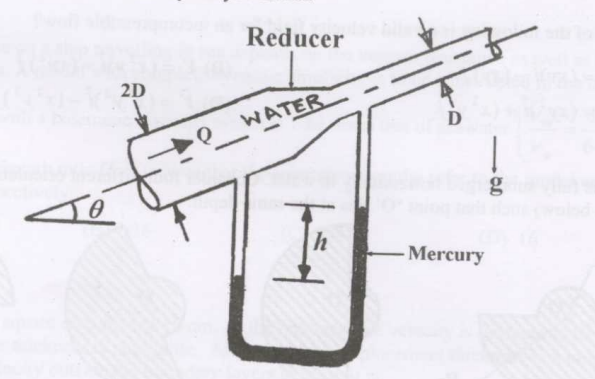
\includegraphics[width=0.5\columnwidth]{figs/ass1_d_q18.png}
  \caption{}
\end{figure} 

\begin{enumerate}
\begin{multicols}{4}
\item  $h_1>h_2>h_3$ 
\item  $h_1<h_2<h_3$ 
\item  $h_1=h_2=h_3$ 
\item  $h_1 =h_3$ and $h_1>h_2$
\end{multicols}
\end{enumerate}

(GATE XE 2008)
\item A $4 m$ wide canal is modelled using a $1 m$ wide dynamically similar model in the laboratory. A wooden block was observed to travel between two points in the model in $8$ seconds. How long will it take to travel between the corresponding points in the actual canal?

\begin{enumerate}
\begin{multicols}{4}
\item  $4 s$ 
\item  $8 s$ 
\item  $16 s$ 
\item  $32 s$
\end{multicols}
\end{enumerate}

(GATE XE 2008)
\item Water (dynamic viscosity $\mu = 0.001 Ns/m^2$) flows under pressure through a pipe of $1 cm$ diameter at a velocity of $1 cm/s$. What would be the head loss per km length of the pipe?

\begin{enumerate}
\begin{multicols}{4}
\item  $0.08 m$ 
\item  $0.16 m$ 
\item  $0.32 m$ 
\item  $1.28 m$
\end{multicols}
\end{enumerate}

(GATE XE 2008)
\item  Air with free stream velocity $10 m/s$ flows over three different bluff bodies P, Q and R as shown below, with a hemisphere of radius $1 m$ forming the nose.

\begin{figure}[H]
\centering
  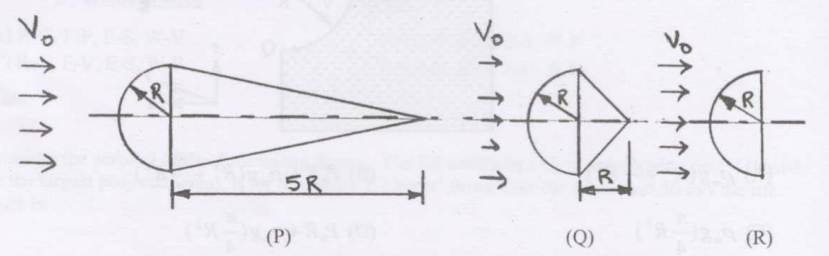
\includegraphics[width=0.7\columnwidth]{figs/ass1_d_q21.png}
  \caption{}
\end{figure} 

Comparing the total drag force $F$ on the three bodies, state which of the following is true.

\begin{enumerate}
\begin{multicols}{4}
\item  $F_P>F_Q>F_R$ 
\item  $F_P=F_Q=F_R$ 
\item  $F_P<F_Q<F_R$ 
\item  $F_P=F_Q and F_R>F_P$
\end{multicols}
\end{enumerate}

(GATE XE 2008)
\item A single engine jet aircraft is in a steady level flight at speed $V_a$ with respect to ground. Assume that the engine intake area ($A_{in}$) is much larger than the engine exhaust area ($A_e$). If the density of the exhaust gas is $\rho _e$ and the exhaust velocity relative to the aircraft is $V_e$, the thrust generated by
the engine is

\begin{enumerate}
\begin{multicols}{4}
\item  $\rho _e V_e ^2 A_e$ 
\item  $\rho _e(V_a +V_e)^2 A_e$ 
\item  $\rho _e(V_a-V_e)^2 A_e$ 
\item  $\rho _e (V_a + V_e) V_e A_e$
\end{multicols}
\end{enumerate}

(GATE XE 2008)
\item Which of the following is a valid velocity field for an incompressible flow?

\begin{enumerate}
\begin{multicols}{2}
\item  $\vec{V} = (xy)\hat{i} - (xy)\hat{j}$
\item  $\vec{V} = (x^2 y)\hat{i} -(xy^2)\hat{j}$
\item  $\vec{V} = (xy^2)\hat{i} +(x^2 y)\hat{j}$
\item  $\vec{V} = (x^2y^2)\hat{i} -(x^2y^2)\hat{j}$
\end{multicols}
\end{enumerate}

(GATE XE 2008)
\item A log is fully submerged horizontally in water. Consider four different orientations (cross-sections shown below) such that point 'O' lies at the same depth.

\begin{figure}[H]
\centering
  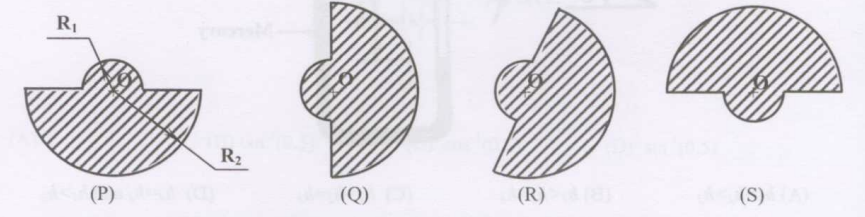
\includegraphics[width=0.7\columnwidth]{figs/ass1_d_q24.png}
  \caption{}
\end{figure} 

Which orientation(s) will give the maximum moment about point O?

\begin{enumerate}
\begin{multicols}{4}
\item  P 
\item  Q 
\item  R 
\item  Pand S
\end{multicols}
\end{enumerate}

(GATE XE 2008)
\item  A closed cylindrical container of diameter D and length L is completely filled with a liquid of density $\rho$. The axis of the cylinder makes an angle with the vertical.

\begin{figure}[H]
\centering
  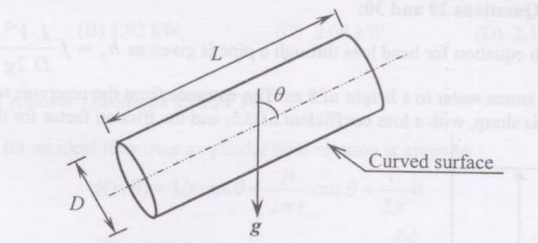
\includegraphics[width=0.5\columnwidth]{figs/ass1_d_q25.png}
  \caption{}
\end{figure} 

The total force on the curved surface is

\begin{enumerate}
\begin{multicols}{2}
\item  $\frac{\pi D^2 L}{4} \rho g \sin{\theta}$
\item  $\frac{\pi D^2 L}{4} \rho g \cos{\theta}$
\item  $\frac{3\pi D^2 L}{4} \rho g \sin{\theta}$
\item  $\frac{3\pi D^2 L}{4} \rho g \cos{\theta}$
\end{multicols}
\end{enumerate}

(GATE XE 2008)
\item  Air flowing over a smooth cylinder of diameter $30 cm$ in a wind tunnel produces a two-dimensional laminar boundary layer that separates from the surface ofthe cylinder. The surface of the cylinder is then roughened with sand paper so that the boundary layer turns turbulent. The location of the point of separation will

\begin{enumerate}
\item  shift upstream

\item  shift downstream

\item  not shift

\item  shift upstream or downstream depending on the roughness height
\end{enumerate}

(GATE XE 2008)
\item The drag force on a ship travelling in sea depends on the viscous resistance as well as the effect of surface waves. A model with complete dynamic similarity is to be constructed in the laboratory using a fluid with a kinematic viscosity which is $\frac{\nu_m}{\nu_p} = \frac{1}{64}$ times that of seawater. What should be the length ratio $\left( \frac{l_m}{l_p} \right)$? Note that the subscripts $m$ and $p$ refer to the model and the prototype respectively.  

\begin{enumerate}
\begin{multicols}{4}
\item  $\frac{1}{64}$  
\item  $\frac{1}{16}$  
\item  $\frac{1}{8}$  
\item  $16$  
\end{multicols}
\end{enumerate}

(GATE XE 2008)
\item Air flows in a square duct of side $10 \ \text{cm}$. At the entrance, the velocity is uniform at $10 \ \text{m/s}$ and the boundary layer thickness is negligible. At the exit, the displacement thickness is $5 \ \text{mm}$ (on each wall). The velocity outside the boundary layers at the exit is:

\begin{enumerate}
\begin{multicols}{4}
\item  $12.35 \ \text{m/s}$  
\item  $11.08 \ \text{m/s}$  
\item  $10 \ \text{m/s}$  
\item  $9 \ \text{m/s}$
\end{multicols}
\end{enumerate}

(GATE XE 2008)
\item[] \textbf{\Large Common Data questions}

\textbf{Common Data for Questions 29 and 30:}  

The Darcy–Weisbach equation for head loss through a pipe is given as  
$h_f = f \frac{L}{D} \frac{V^2}{2g}$.  

A reservoir, as shown in the figure, stores water to a height of $8 \ \text{m}$.  
The entrance from the reservoir to the pipe (length $50 \ \text{m}$, diameter $10 \ \text{cm}$) is sharp, with a loss coefficient of $0.5$, and the friction factor for the pipe is $0.017$.  

\begin{figure}[H]
\centering
  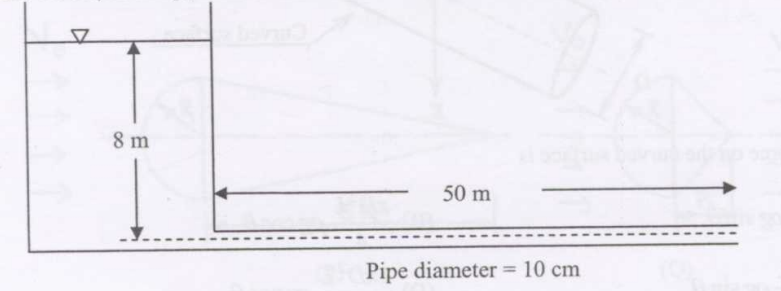
\includegraphics[width=0.5\columnwidth]{figs/ass1_d_q29.png}
  \caption{}
\end{figure} 

\item What would be the discharge through the pipe?  

\begin{enumerate}
\begin{multicols}{4}
\item  $0.0314 \ \text{m}^3/\text{s}$  
\item  $0.0322 \ \text{m}^3/\text{s}$  
\item  $0.0331 \ \text{m}^3/\text{s}$  
\item  $0.0341 \ \text{m}^3/\text{s}$  
\end{multicols}
\end{enumerate}

(GATE XE 2008)

\item If it is desired to increase the discharge, the following four options are available:  

1. Increase the pipe length, keeping everything else the same  

2. Increase the pipe diameter, keeping everything else the same  

3. Add a valve at the end of the pipe, keeping everything else the same 

4. Replace the sharp entrance by a rounded entrance, keeping everything else the same  

Only two of these options serve our purpose. Which are they?  

\begin{enumerate}
\begin{multicols}{4}
\item  1, 2  
\item  1, 3  
\item  2, 4  
\item  3, 4 
\end{multicols}
\end{enumerate}

(GATE XE 2008)

\item[] \textbf{\Large Linked Answer Questions: Q.31 to Q.34 carry two marks each.}

\textbf{Statement for Linked Answer Questions 31 and 32:}  

A pump draws water from a reservoir and discharges it to an overhead tank as shown.  
The area of the outlet pipe is $20 \ \text{cm}^2$ and the average velocity in the outlet pipe is $3 \ \text{m/s}$.  
Neglect the minor and major losses in the piping.  

\begin{figure}[H]
\centering
  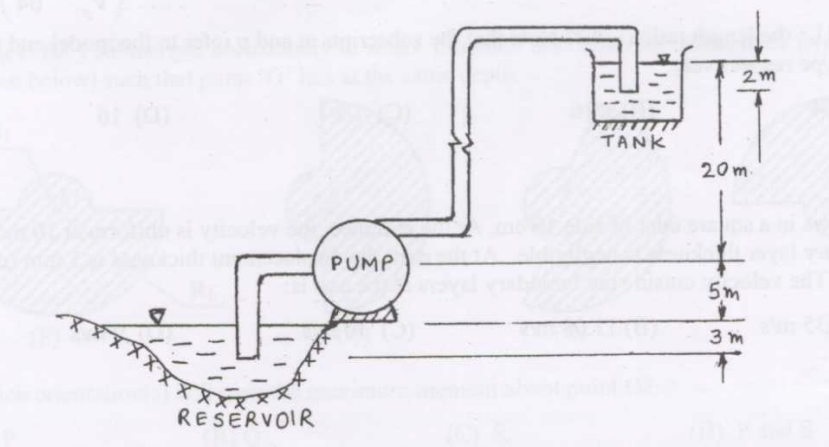
\includegraphics[width=0.8\columnwidth]{figs/ass1_d_q31.png}
  \caption{}
\end{figure}

\item The total head developed by the pump (in metres of water) is:  

\begin{enumerate}
\begin{multicols}{4}
\item  $27 \ \text{m}$  
\item  $25 \ \text{m}$  
\item  $24 \ \text{m}$  
\item  $22 \ \text{m}$  
\end{multicols}
\end{enumerate}

(GATE XE 2008)


\item If the combined efficiency of the pump and motor is $0.75$, then the power required to run the pump is:  

\begin{enumerate}
\begin{multicols}{4}
\item  $1.76 \ \text{kW}$  
\item  $1.92 \ \text{kW}$  
\item  $2.00 \ \text{kW}$  
\item  $2.16 \ \text{kW}$ 
\end{multicols}
\end{enumerate}

(GATE XE 2008)

\item[] \textbf{Statement for Linked Answer Questions 33 and 34:}  

The potential function for an ideal flow over a cylinder with rotation is given by  
$\phi(r,\theta) = U r \cos \theta + \frac{\mu}{2 \pi r} \cos \theta + \frac{\Gamma}{2\pi} \theta$  

The velocity components are related to the potential function as  
$u_r = \frac{\partial \phi}{\partial r}$ and $u_\theta = \frac{1}{r} \frac{\partial \phi}{\partial \theta}$.  

\begin{figure}[H]
\centering
  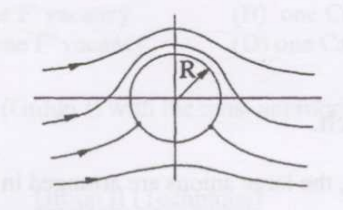
\includegraphics[width=0.5\columnwidth]{figs/ass1_d_q33.png}
  \caption{}
\end{figure}

\item What is the radius of the cylinder?  

\begin{enumerate}
\begin{multicols}{4}
\item  $R = \sqrt{\frac{\mu}{2 \pi U}}$  
\item  $R = \sqrt{\frac{2 \pi U}{\mu}}$  
\item  $R = \sqrt{\frac{\mu}{\Gamma - 2 \pi U}}$  
\item  $R = \sqrt{\frac{\Gamma - 2 \pi U}{\mu}}$  
\end{multicols}
\end{enumerate}

(GATE XE 2008)

\item Where are the stagnation points located?  

\begin{enumerate}
\begin{multicols}{4}
\item  $\theta = 0$ and $\theta = \pi$  

\item  $\theta = \sin^{-1} \left( \frac{\Gamma}{4 \pi U R} \right)$ and $\theta = \pi - \sin^{-1} \left( \frac{\Gamma}{4 \pi U R} \right)$  

\item  $\theta = \frac{\pi}{2}$ and $\theta = -\frac{\pi}{2}$  

\item  $\theta = \cos^{-1} \left( \frac{\Gamma}{4 \pi U R} \right)$ and $\theta = 2\pi - \cos^{-1} \left( \frac{\Gamma}{4 \pi U R} \right)$  
\end{multicols}
\end{enumerate}

(GATE XE 2008)
\end{enumerate}
\begin{center}
    \textbf{END OF SECTION - D}
\end{center}

\newpage

\begin{center}
    \textbf{\Large E : MATERIALS SCIENCE}
\end{center}

\textbf{Useful Data}

   \begin{table}[H]     \centering     \caption{}     \label{}     \begin{tabular}{ll}
Avogadro's number & $6.023 \times 10^{23} \ \text{mol}^{-1}$ \\
Boltzmann's constant & $1.38 \times 10^{-23} \ \text{J K}^{-1}$ \\
Electron charge & $1.6 \times 10^{-19} \ \text{C}$ \\
Gas constant & $8.314 \ \text{J mol}^{-1} \text{K}^{-1}$ \\
Electron rest mass & $9.1 \times 10^{-31} \ \text{kg}$ \\
Free space permittivity $(\varepsilon_0)$ & $8.854 \times 10^{-12} \ \text{F m}^{-1}$ or $\text{C} \ \text{V}^{-1} \ \text{m}^{-1}$ \\
Free space magnetic permeability $(\mu_0)$ & $4\pi \times 10^{-7} \ \text{H m}^{-1}$ \\
Speed of light $(c)$ & $3 \times 10^{8} \ \text{m s}^{-1}$ \\
Planck's constant $(h)$ & $6.62 \times 10^{-34} \ \text{J s}$ \\
Bohr magneton, $\mu_B$ & $9.27 \times 10^{-24} \ \text{A m}^2$ \\
\end{tabular} \end{table}


$1 \ \text{eV} = 1.6 \times 10^{-19} \ \text{J}$ \\
$1 \ \text{cal} = 4.2 \ \text{J}$

\begin{enumerate}
\item[] \textbf{Q1 - Q8 carry one mark each}

\item In the rocksalt-type structure, the large anions are arranged in a cubic close-packed manner. The cations occupy

\begin{enumerate}

\item  all the octahedral interstitial sites
\item  half of the octahedral interstitial sites and quarter of the tetrahedral interstitial sites
\item  all the tetrahedral interstitial sites
\item  50\% of the tetrahedral interstitial sites
\end{enumerate}

(GATE XE 2008)
\item  Which of the following is \textbf{\underline NOT} a Bravais lattice?

\begin{enumerate}
\begin{multicols}{2}
\item  Body-centered tetragonal 
\item  Face-centered tetragonal
\item  Body-centered orthorhombic 
\item  Face-centered orthorhombic
\end{multicols}
\end{enumerate}

(GATE XE 2008)
\item The characteristic diffusion distance in a material with diffusivity $D$ in time $t$ is proportional to  

\begin{enumerate}
\begin{multicols}{4}
    \item  $D t^{1/2}$  
    \item  $D^{1/2} t$  
    \item  $D^{1/2} t^{1/2}$  
    \item  $D t$ 
\end{multicols}
\end{enumerate}

    (GATE XE 2008)  
\item At constant pressure, the maximum degrees of freedom in a binary phase diagram are  

\begin{enumerate}
\begin{multicols}{4}
    \item  $0$  
    \item  $1$  
    \item  $2$  
    \item  $3$
\end{multicols}
\end{enumerate}

    (GATE XE 2008)  
\item When the particle size decreases, the surface-to-volume ratio  

\begin{enumerate}
\begin{multicols}{2}
    \item  increases  
    \item  decreases  
    \item  remains constant  
    \item  is material-dependent 
\end{multicols}
\end{enumerate}

    (GATE XE 2008)  
\item A material in the superconducting state is  

\begin{enumerate}
\begin{multicols}{4}
    \item  paramagnetic  
    \item  diamagnetic  
    \item  ferromagnetic  
    \item  antiferromagnetic 
\end{multicols}
\end{enumerate}

    (GATE XE 2008)  
\item Toughness is a measure of  

\begin{enumerate}
\item  the stress required to fracture a material  
\item  the strain required to fracture a material 
\item  the energy required to fracture a material 
\item  the energy required to plastically deform a material 
\end{enumerate}

    (GATE XE 2008)  
\item Metals, because of their many available empty electron states, will absorb  

\begin{enumerate}
\item  X- and $\gamma$-ray radiation  
\item  visible light of all frequencies  
\item  ultra-violet (UV) light  
\item  all the frequencies greater than that of UV light 
\end{enumerate}    

    (GATE XE 2008)  

\item[] \textbf{Q. 9 to Q.30 carry two marks each.}
\item The stacking sequence of the (001) FCC and (0001) HCP planes is  

\begin{enumerate}
\begin{multicols}{2}
\item  $\ldots$ABAB and ABAB$\ldots$  
\item  $\ldots$ABCABC and ABCABC$\ldots$  
\item  $\ldots$ABAB and ABCABC$\ldots$  
\item  $\ldots$ABCABC and ABAB$\ldots$  
\end{multicols}
\end{enumerate}

(GATE XE 2008)

\item A Schottky defect in CaF$_2$ is comprised of  

\begin{enumerate}
\begin{multicols}{2}
\item  one Ca$^{2+}$ vacancy and one F$^-$ \newline vacancy  
\item  one Ca$^{2+}$ vacancy and one F$^-$ \newline interstitial  
\item  two Ca$^{2+}$ vacancies and one F$^-$ vacancy  
\item  one Ca$^{2+}$ vacancy and two F$^-$ vacancies  
\end{multicols}
\end{enumerate}

(GATE XE 2008)

\item Match the materials property (Group I) with the most appropriate characterization technique (Group II).  

\begin{table}[H]     \centering     \caption{}     \label{}     \begin{tabular}{l l}
\textbf{Group I (Property)} & \textbf{Group II (Technique)}  \\
P)Lattice strain & 1) Scanning electron microscope  \\
Q) Band Gap & 2) X-ray diffraction  \\
R) Surface topography & 3) Optical Absorption Spectroscopy \\ 
S) Specific Heat &4) Differential Scanning Calorimetry  \\
   & 5) Nuclear Magnetic Resonance (NMR) Spectroscopy  
\end{tabular} \end{table}
\begin{enumerate}
\begin{multicols}{2}
\item  P-1, Q-2, R-3, S-4  
\item  P-5, Q-1, R-2, S-3  
\item  P-2, Q-3, R-1, S-4  
\item  P-3, Q-5, R-1, S-4  
\end{multicols}
\end{enumerate}
(GATE XE 2008)

\item The average degree of polymerization of Polypropylene associated with an average molecular weight of $36000$ amu is (atomic masses of C and H are $12$ and $1$ amu, respectively)  

\begin{enumerate}
\begin{multicols}{4}
\item  $1286$  
\item  $857$  
\item  $360$  
\item  $346$  
\end{multicols}
\end{enumerate}

 (GATE XE 2008)

\item In an alloy system, X-Y, three phases $\alpha$ (10), $\gamma$ (21), and L$_{\text{iq}}$ (45) are in equilibrium at $700^\circ$C and $\gamma$ (21), L$_{\text{iq}}$ (68) and $\beta$ (89) are in equilibrium at $420^\circ$C. (Numbers in the brackets are compositions of the phase in wt\% of X). Choose the \textbf{\underline INCORRECT} statement:  

\begin{enumerate}
\item  $\gamma$ is an intermetallic compound  
\item  Equilibrium at $700^\circ$C is peritectic  
\item  Equilibrium at $420^\circ$C is eutectic  
\item  Equilibrium at $420^\circ$C is eutectoid  
\end{enumerate}

(GATE XE 2008)

\item Which one of the following may \textbf{\underline NOT} help in resisting the weld decay or intergranular corrosion in austenitic stainless steel?  

\begin{enumerate}

\item  Heating the stainless steel to $1000^\circ$C followed by quenching to room temperature  
\item  Heating the stainless steel to $1000^\circ$C followed by furnace cooling 
\item  Lowering the carbon content to $0.03$ wt.\% in the stainless steel  
\item  Alloying the stainless steel with Nb or Ti  
\end{enumerate}

(GATE XE 2008)

\item A badminton racquet stem is designed to have a Young’s modulus of $230$ GPa. The stem is made up of long, oriented carbon fibres parallel to the stem axis in an epoxy matrix. The Young’s moduli of carbon fibre and epoxy are $400$ GPa and $3$ GPa respectively. The volume fraction of the fiber in the composite should be  

\begin{enumerate}
\begin{multicols}{4}
\item  $0.006$  
\item  $0.428$  
\item  $0.572$  
\item  $0.994$  
\end{multicols}
\end{enumerate}

(GATE XE 2008)


\item Match the material (Group I) with its most well known application (Group II).

\begin{table}[H]     \centering     \caption{}     \label{}     \begin{tabular}{l l}
\textbf{Group I (Material)} & \textbf{Group II (Application)} \\
P) Graphite & 1) Lubricant \\
Q) Cermet & 2) Cutting tools \\
R) PbS & 3) Infrared detector \\
S) Quartz & 4) Crystal oscillator \\
 & 5) Red LED \\
\end{tabular} \end{table}

\begin{enumerate}
\begin{multicols}{2}
\item  P-1, Q-2, R-3, S-4
\item  P-3, Q-1, R-2, S-4
\item  P-5, Q-1, R-2, S-3
\item  P-2, Q-5, R-1, S-4
\end{multicols}
\end{enumerate}

(GATE XE 2008)

\item At constant volume, the energy required to raise the temperature of $1 \ \mathrm{g}$ of a monatomic solid (atomic mass: $24 \ \mathrm{amu}$) by $1^\circ \mathrm{C}$ at $T \gg \Theta_{\mathrm{Debye}}$ is:

\begin{enumerate}
\begin{multicols}{4}
\item  $0.20 \ \mathrm{cal}$ 
\item  $0.25 \ \mathrm{cal}$ 
\item  $0.30 \ \mathrm{cal}$ 
\item  $0.35 \ \mathrm{cal}$
\end{multicols}
\end{enumerate}

(GATE XE 2008)

\item For a hard magnet, the remnant induction $(B_r)$ is $0.5 \ \mathrm{T}$ and the coercive field $(H_c)$ is $4 \times 10^4 \ \mathrm{A \, m^{-1}}$. The energy loss of the magnet per cycle is:

\begin{enumerate}
\begin{multicols}{4}
\item  $2 \ \mathrm{kJ \, m^{-3}}$
\item  $20 \ \mathrm{kJ \, m^{-3}}$
\item  $40 \ \mathrm{kJ \, m^{-3}}$
\item  $80 \ \mathrm{kJ \, m^{-3}}$
\end{multicols}
\end{enumerate}

(GATE XE 2008)

\item A $1 \ \mathrm{mm}$ thick sheet of a material having a relative dielectric constant of $4$ is subjected to a static voltage of $100 \ \mathrm{V}$. The polarization induced in the sheet is:

\begin{enumerate}
\begin{multicols}{4}
\item  $3 \times 10^{-6} \ \mathrm{C \, m^{-2}}$
\item  $2.7 \times 10^{-6} \ \mathrm{C \, m^{-2}}$
\item  $4.2 \times 10^{-7} \ \mathrm{C \, m^{-2}}$
\item  $6.8 \times 10^{-5} \ \mathrm{C \, m^{-2}}$
\end{multicols}
\end{enumerate}

(GATE XE 2008)

\item The refractive index of a window glass is $1.5$ in the range of visible wavelengths of light. The value of the reflectivity is:

\begin{enumerate}
\begin{multicols}{4}
\item  $0.01$ 
\item  $2$ 
\item  $0.04$
\item  $5$
\end{multicols}
\end{enumerate}

(GATE XE 2008)

\item In BaTiO$_3$, the presence of spontaneous polarization is as a result of the

\begin{enumerate}

\item  relative displacements of the Ti$^{4+}$ and O$^{2-}$ ions from their symmetrical positions 
\item  displacement of only cations from their symmetrical positions
\item  relative displacements of Ba$^{2+}$ and O$^{2-}$ ions from their symmetrical positions
\item  displacement of only O$^{2-}$ ions from their symmetrical positions
\end{enumerate}

(GATE XE 2008)

\item What is the yield strength of a material with a grain size of $10 \ \mu \mathrm{m}$? The yield strength of a single crystal of this material is $80 \ \mathrm{MPa}$ and its Hall–Petch constant is $0.6 \ \mathrm{MN \, m^{-3/2}}$.

\begin{enumerate}
\begin{multicols}{4}
\item  $80 \ \mathrm{MPa}$ 
\item  $86 \ \mathrm{MPa}$ 
\item  $140 \ \mathrm{MPa}$
\item  $270 \ \mathrm{MPa}$
\end{multicols}
\end{enumerate}

(GATE XE 2008)

\item The amount of sulphur (S) required for $5\%$ cross linking in $100 \ \mathrm{kg}$ of polyisoprene is (atomic masses of H, C, and S are $1$, $12$, and $32 \ \mathrm{amu}$, respectively):

\begin{enumerate}
\begin{multicols}{4}
\item  $23.5 \ \mathrm{g}$ \quad
\item  $47 \ \mathrm{g}$ \quad
\item  $2.35 \ \mathrm{kg}$ \quad
\item  $16 \ \mathrm{kg}$
\end{multicols}
\end{enumerate}

(GATE XE 2008)

\item Match the type of laser (Group I) with its lasing medium (Group II).

\begin{table}[H]     \centering     \caption{}     \label{}     \begin{tabular}{l l}
\textbf{Group I (Laser)} & \textbf{Group II (Lasing Medium)} \\
P) CO$_2$ & 1) Gas \\
Q) Ruby & 2) Metal vapor \\
R) Dye & 3) Liquid \\
S) HeCd & 4) Solid \\
 & 5) Gas-ions \\
\end{tabular} \end{table}

\begin{enumerate}
\begin{multicols}{2}
\item  P-1, Q-4, R-3, S-2 
\item  P-1, Q-2, R-3, S-4 
\item  P-2, Q-4, R-5, S-4 
\item  P-5, Q-4, R-3, S-4 
\end{multicols}
\end{enumerate}

(GATE XE 2008)

\item Which of the following is the direction common to $(\bar{1}11)$ and $(111)$ planes?

\begin{enumerate}
\begin{multicols}{4}
\item  $[011]$ 
\item  $[21\bar{1}]$ 
\item  $[0\bar{1}1]$ 
\item  $[001]$ 
\end{multicols}
\end{enumerate}

(GATE XE 2008)

\item The net magnetic moment of iron (Fe) is $2.22 \, \mu_B$ per atom. Calculate the saturation flux density in iron. (Density of iron: $7.87 \, \mathrm{g/cm^3}$; Atomic mass of iron: $56 \, \mathrm{amu}$)

\begin{enumerate}
\begin{multicols}{4}
\item  $2.18 \times 10^{-6} \ \mathrm{Tesla}$ 
\item  $2.18 \times 10^{-12} \ \mathrm{Tesla}$ 
\item  $2.18 \times 10^{9} \ \mathrm{Tesla}$ 
\item  $2.18 \ \mathrm{Tesla}$ 
\end{multicols}
\end{enumerate}

(GATE XE 2008)



\item[] \textbf{\Large Common Data Questions}
\textbf{Common Data for Questions 27 and 28:}

A hypothetical load–elongation curve for a $13 \ \mathrm{mm}$ diameter tensile specimen with $50 \ \mathrm{mm}$ gauge length is as shown.

\begin{figure}[H]
\centering
  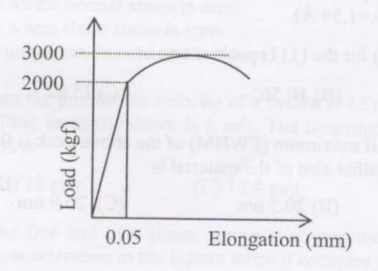
\includegraphics[width=0.5\columnwidth]{figs/ass1_e_q27.png}
  \caption{}
\end{figure} 


\item The Young’s modulus is

\begin{enumerate}
\begin{multicols}{4}
\item  $101 \ \mathrm{GPa}$ 
\item  $148 \ \mathrm{GPa}$ 
\item  $201 \ \mathrm{GPa}$ 
\item  $301 \ \mathrm{GPa}$ 
\end{multicols}
\end{enumerate}

(GATE XE 2008)

\item The ultimate tensile strength of the material is

\begin{enumerate}
\begin{multicols}{4}
\item  $207 \ \mathrm{MPa}$ 
\item  $247 \ \mathrm{MPa}$ 
\item  $222 \ \mathrm{MPa}$ 
\item  $267 \ \mathrm{MPa}$ 
\end{multicols}
\end{enumerate}

(GATE XE 2008)



\item[] \textbf{Common Data for Questions 29 and 30:}

A cylindrical well-annealed copper (Cu) specimen having a cross-sectional area of $5 \times 10^{-6} \ \mathrm{m^2}$ and length of $1 \ \mathrm{m}$ has a dislocation density of $10^{9} \ \mathrm{m^{-2}}$ and grain diameter of $40 \ \mu\mathrm{m}$. This specimen is reduced to a cross-section of $1 \times 10^{-6} \ \mathrm{m^2}$ by passing through a die and in the process, its dislocation density increases to $10^{13} \ \mathrm{m^{-2}}$. Subsequently, the wire is annealed at $400^\circ \mathrm{C}$ and the just-recrystallized wire has a grain diameter of $10 \ \mu\mathrm{m}$. If it is kept at $450^\circ \mathrm{C}$ for a longer duration, grain growth would occur. (Shear modulus of Cu: $44 \ \mathrm{GPa}$; Atomic diameter of Cu: $2.56 \ \mathrm{\AA}$; Specific grain boundary energy of Cu: $0.5 \ \mathrm{J/m^2}$)



\item What is the strain energy stored in the just-deformed copper specimen?

\begin{enumerate}
\begin{multicols}{4}
\item  $72 \ \mathrm{J}$ 
\item  $36 \ \mathrm{J}$ 
\item  $72 \ \mathrm{mJ}$ 
\item  $36 \ \mathrm{mJ}$ 
\end{multicols}
\end{enumerate}

(GATE XE 2008)

\item What is the driving force for grain growth (stored grain boundary energy) just after recrystallization at $450^\circ \mathrm{C}$ in the given specimen?

\begin{enumerate}
\begin{multicols}{4}
\item  $375 \ \mathrm{mJ}$ 
\item  $750 \ \mathrm{mJ}$ 
\item  $1.5 \ \mathrm{J}$ 
\item  $3.0 \ \mathrm{J}$ 
\end{multicols}
\end{enumerate}

(GATE XE 2008)

\item[]\textbf{\Large Linked Answer Questions: Q.31 to Q.34 (carry two marks each)} 

\textbf{Statement for Linked Answer Questions 31 and 32:} 

    For a semiconductor, the electron and hole mobilities are $\mu_e = 0.364 \ \mathrm{m^2 \, V^{-1} \, s^{-1}}$, $\mu_h = 0.19 \ \mathrm{m^2 \, V^{-1} \, s^{-1}}$, and the intrinsic carrier concentrations are $n_e = n_h = 2.3 \times 10^{19} \ \mathrm{m^{-3}}$ at $300 \ \mathrm{K}$.

\item The electrical conductivity of the semiconductor at $300 \ \mathrm{K}$ is

\begin{enumerate}
\begin{multicols}{4}
\item  2.04 $\mathrm{\Omega^{-1} \, m^{-1}}$
\item  1.34 $\mathrm{\Omega^{-1} \, m^{-1}}$
\item  0.70 $\mathrm{\Omega^{-1} \, m^{-1}}$
\item  2.74 $\mathrm{\Omega^{-1} \, m^{-1}}$
\end{multicols}
\end{enumerate}

    (GATE XE 2008)

    \item Upon increasing the temperature to $373 \ \mathrm{K}$, the electrical conductivity increases to $25.75 \ \mathrm{\Omega^{-1} \, m^{-1}}$. The bandgap of the semiconductor is

\begin{enumerate}
\begin{multicols}{4}
\item 1.43 eV
\item 1.11 eV
\item 0.67 eV
\item 0.33 eV
\end{multicols}
\end{enumerate}
    
    (GATE XE 2008)

    \item[] \textbf{Statement for Linked Answer Questions 33 and 34:} 

    The X-ray powder diffraction pattern of a well annealed cubic material (lattice parameter $a = 4.2 \ \mathrm{\AA}$) is taken using CuK$_\alpha$ radiation ($\lambda = 1.54 \ \mathrm{\AA}$).

    \item The Bragg angle ($\theta_B$) for the (111) peak occurs at

\begin{enumerate}
\begin{multicols}{4}
\item  $18.55^{\circ}$
\item  $10.56^{\circ}$
\item  $15.02^{\circ}$
\item  $33.37^{\circ}$
\end{multicols}
\end{enumerate}
   
    (GATE XE 2008)

    \item If the full width at half maximum (FWHM) of the above peak is $0.4^{\circ}$, ignoring the instrumental broadening, the crystallite size of the material is

\begin{enumerate}
\begin{multicols}{4}
\item  20.2 nm
\item  20.5 nm
\item  20.9 nm
\item  23.7 nm
\end{multicols}
\end{enumerate}
    
    (GATE XE 2008)

\end{enumerate}    
\begin{center}
    \textbf{END OF SECTION - E}
\end{center}

\newpage

\begin{center}
    \textbf{\Large F : SOLID MECHANICS}
\end{center}

\begin{enumerate}
\item[] \textbf{Q1 - Q8 carry one mark each}

\item Which of the following is true?  

\begin{enumerate}

\item  In the plane of maximum shear, normal stress is always zero.
\item  In the plane of maximum shear, normal stress may not be always zero.
\item  In a principal plane, shear stress is never zero.
\item  In a principal plane, normal stress is always zero. 
\end{enumerate}

(GATE XE 2008)

\item State of stress at a point in a loaded body is given by $\sigma_x = 10 \ \text{MPa}$, $\sigma_y = 0$, $\sigma_z = -5 \ \text{MPa}$ and $\tau_{xy} = \tau_{yz} = \tau_{zx} = 0$. Maximum shear stress at that point is  

\begin{enumerate}
\begin{multicols}{4}
\item  $5 \ \text{MPa}$  
\item  $2.5 \ \text{MPa}$  
\item  $7.5 \ \text{MPa}$  
\item  $0$  
\end{multicols}
\end{enumerate}

(GATE XE 2008)

\item State of stress at a point of a body in a plane stress problem is given by $\sigma_x = -6 \ \text{MPa}$, $\sigma_y = 2 \ \text{MPa}$ and $\tau_{xy} = \text{MPa}$. Which of the following is true at that point?  

\begin{enumerate}
\item  There exists at least one plane where normal stress is zero. 
\item  There exists no plane where normal stress is zero.  
\item  There exists no plane where shear stress is zero.  
\item  In the plane of maximum shear, normal stress is zero. 
\end{enumerate}

(GATE XE 2008)

\item To an observer standing on the ground the velocity of a cyclist is $12 \ \text{m/s}$ in the horizontal direction and that of rain drops falling vertically down is $6 \ \text{m/s}$. The magnitude of the velocity of the rain drops relative to the cyclist is  

\begin{enumerate}
\begin{multicols}{4}
\item  $6 \ \text{m/s}$  
\item  $12 \ \text{m/s}$  
\item  $13.4 \ \text{m/s}$  
\item  $18.4 \ \text{m/s}$  
\end{multicols}
\end{enumerate}

(GATE XE 2008)

\item If a mass attached to the free end of a linear spring is so constrained that it executes vertical undamped oscillations, its acceleration at the instant when it occupies the static equilibrium position is  

\begin{enumerate}
\begin{multicols}{2}
\item  vertically upward  
\item  vertically downward  
\item  the maximum  
\item  zero  
\end{multicols}
\end{enumerate}

(GATE XE 2008)

\item If three nonparallel forces are in equilibrium they  

\begin{enumerate}
\item  must be concurrent but need not be coplanar  
\item  must be coplanar but need not be concurrent  
\item  must be both concurrent and coplanar  
\item  need not have zero as the geometric sum of the force vectors  
\end{enumerate}

(GATE XE 2008)

\item A point of contraflexure in a loaded beam is one where 

\begin{enumerate}
\begin{multicols}{2}
\item  shear force is maximum.  
\item  shear force and bending moment are maximum.  
\item  bending moment is maximum.  
\item  bending moment is zero.  
\end{multicols}
\end{enumerate}

(GATE XE 2008)

\item In a beam of uniform strength, the extreme fibers at every cross section are stressed to the maximum allowable stress. Consider a solid circular beam of uniform strength subjected to bending moment. In this beam, the diameter of the cross-section at any section is proportional  

\begin{enumerate}
\item  to cube root of the bending moment at that section. 
\item  to the square root of the bending moment at that section.  
\item  to the bending moment at that section.  
\item  inversely to the bending moment at that section. 
\end{enumerate}

(GATE XE 2008)

\item[] \textbf{Q9 to Q30 carry two marks each.}


\item For a loaded body representing a two dimensional plane problem, the displacement components along $x$ and $y$ at any point $(x, y)$ are $u = x^2 + y^2$, $v = 2xy$ respectively. Principal strains at the point $(3, 1)$ in the body are 

\begin{enumerate}
\begin{multicols}{2}
\item  $\epsilon_1 = 8, \epsilon_2 = 2$  
\item  $\epsilon_1 = 6.24, \epsilon_2 = 1.76$  
\item  $\epsilon_1 = 0, \epsilon_2 = 3$  
\item  $\epsilon_1 = 5, \epsilon_2 = -3$  
\end{multicols}
\end{enumerate}

(GATE XE 2008)  

\item A $9 \ \text{kN}$ tensile load will be applied to a $50 \ \text{m}$ length steel wire with $E = 200 \ \text{GPa}$. The normal stress in the wire must not exceed $150 \ \text{MPa}$ and the increase in the length of the wire should be at most $25 \ \text{mm}$. Which among these could be the smallest diameter of the wire so that the wire does not fail?  

\begin{enumerate}
\begin{multicols}{4}
\item  $5.75 \ \text{mm}$  
\item  $7.75 \ \text{mm}$  
\item  $8.75 \ \text{mm}$  
\item  $10.7 \ \text{mm}$  
\end{multicols}
\end{enumerate}

(GATE XE 2008)  

\item A uniform circular cross section rod made of a brittle material is subjected to a pure torsion. If $d$ is the diameter of the cross section of the rod and $\sigma_{\text{all}}$ is the maximum allowable normal stress for the material of the rod, then the maximum twisting moment that can be applied to the rod without failure is  

\begin{enumerate}
\begin{multicols}{2}
\item  $\frac{\sigma_{\text{all}}}{16} \pi d^3$  
\item  $\frac{\sigma_{\text{all}}}{32} \pi d^3$  
\item  $\frac{\sigma_{\text{all}}}{8} \pi d^3$  
\item  $\frac{\sigma_{\text{all}}}{64} \pi d^3$ 
\end{multicols}
\end{enumerate}

(GATE XE 2008)  

\item A thin walled spherical pressure vessel of mean radius $1000 \ \text{mm}$, having a wall thickness of $10 \ \text{mm}$ is subjected to an internal pressure of $0.8 \ \text{MPa}$. The maximum shear stress developed in the wall will be  

\begin{enumerate}
\begin{multicols}{4}
\item  $0$  
\item  $20 \ \text{MPa}$  
\item  $40 \ \text{MPa}$  
\item  $80 \ \text{MPa}$
\end{multicols}
\end{enumerate}

(GATE XE 2008)  

\item A rectangular cross section beam of width $w = 0.25 \ \text{m}$ and depth $d = 0.4 \ \text{m}$ is subjected to a bending moment $M = 200 \ \text{N} \cdot \text{m}$ and a uniform axial load of $P = 200 \ \text{N}$ as shown. Measured from the centroidal axis of the beam, normal stress will be zero at a distance of  

\begin{figure}[H]
\centering
  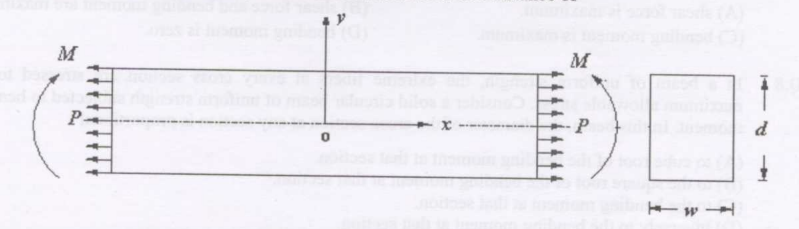
\includegraphics[width=0.7\columnwidth]{figs/ass1_f_q13.png}
  \caption{}
\end{figure}

\begin{enumerate}
\begin{multicols}{4}
\item  $y = 15 \ \text{mm}$  
\item  $y = -13.3 \ \text{mm}$  
\item  $y = -15 \ \text{mm}$  
\item  $y = 10 \ \text{mm}$  
\end{multicols}
\end{enumerate}

(GATE XE 2008)  


    \item Three masses $M$, $2M$ and $3M$ are attached by circular cross section wires and are rotated around a vertical axis on a frictionless plane at 4 Hz as shown in the figure. Consider the masses to be concentrated as points. For equal stresses in wires in all the three segments, the cross sectional areas of the wires in the three segments 1, 2 and 3 should be in the ratio

    \begin{figure}[H]
\centering
  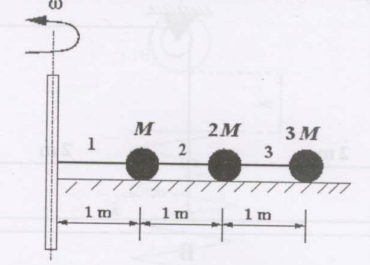
\includegraphics[width=0.5\columnwidth]{figs/ass1_f_q14.png}
  \caption{}
\end{figure}

\begin{enumerate}
\begin{multicols}{4}
\item  1:2:3
\item  3:2:1
\item  9:4:1
\item  14:13:9
\end{multicols}
\end{enumerate}
    
    (GATE XE 2008)
    
    \item Two steel plates of uniform cross section $10 \ \mathrm{mm} \times 80 \ \mathrm{mm}$ are welded together and subjected to an axial load of $P=100 \ \mathrm{kN}$ as shown in the figure. Allowable normal stress (tension and compression) and allowable shear stress for the material of the weld are 100 MPa and 50 MPa respectively and $\beta = 25^\circ$. Which of the following is true?

    \begin{figure}[H]
\centering
  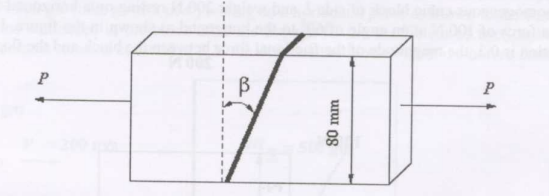
\includegraphics[width=0.7\columnwidth]{figs/ass1_f_q15.png}
  \caption{}
\end{figure}

\begin{enumerate}
\item  The joint will fail due to normal tensile stress.
\item  The joint will fail due to normal compressive stress.
\item  The joint will fail due to shear stress.
\item  The joint will not fail.
\end{enumerate}
    
    (GATE XE 2008)
    
    \item A plane cantilever truss is loaded as shown in the figure. If a positive sign denotes tension and a negative sign compression, the axial force in the member 1 is

     \begin{figure}[H]
    \centering
    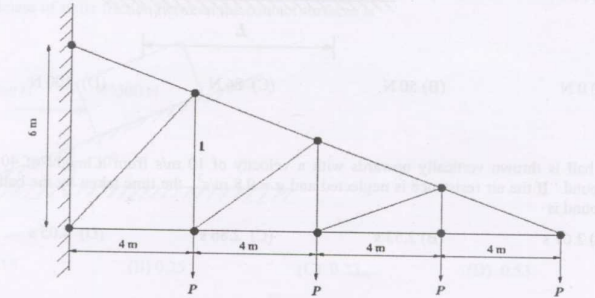
\includegraphics[width=0.7\columnwidth]{figs/ass1_f_q16.png}
    \caption{}
\end{figure}

\begin{enumerate}
\begin{multicols}{4}    
\item  $-5.33P$
\item  $-1.67P$
\item  $+2P$
\item  $+3P$
\end{multicols}
\end{enumerate}
    
    (GATE XE 2008)


    \item A man weighing $600 \ \mathrm{N}$ stands on a horizontal beam of negligible weight at C and holds a string passing over two smooth pulleys and attached to point B on the beam as shown in the figure. The tension in the string is

    \begin{figure}[H]
    \centering
    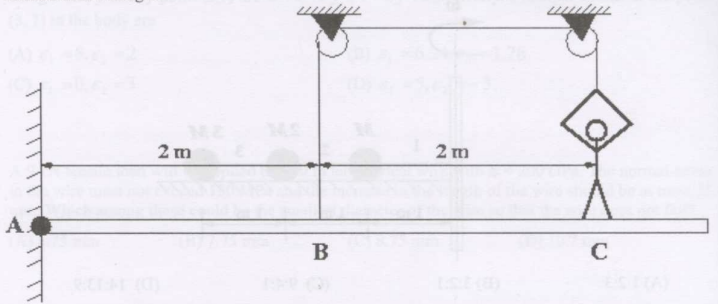
\includegraphics[width=0.5\columnwidth]{figs/ass1_f_q17.png}
    \caption{}
    \end{figure}

\begin{enumerate}
\begin{multicols}{4}
    \item  $100 \ \mathrm{N}$ \quad
    \item  $400 \ \mathrm{N}$ \quad
    \item  $600 \ \mathrm{N}$ \quad
    \item  $1200 \ \mathrm{N}$
\end{multicols}
\end{enumerate}

    (GATE XE 2008)

    \item A homogeneous cubic block of side $L$ and weight $200 \ \mathrm{N}$ resting on a horizontal floor is acted upon by a force of $100 \ \mathrm{N}$ at an angle of $60^{\circ}$ to the horizontal as shown in the figure. If the coefficient of friction is $0.3$, the magnitude of the frictional force between the block and the floor is

    \begin{figure}[H]
    \centering
    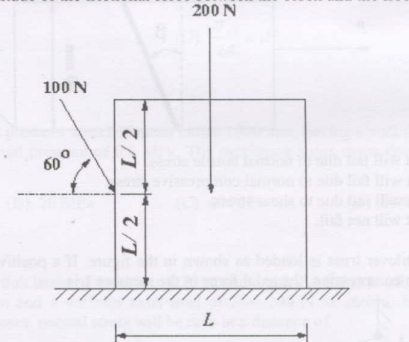
\includegraphics[width=0.5\columnwidth]{figs/ass1_f_q18.png}
    \caption{}
    \end{figure}

\begin{enumerate}
\begin{multicols}{4}
    \item  $0 \ \mathrm{N}$ \quad
    \item  $50 \ \mathrm{N}$ \quad
    \item  $86 \ \mathrm{N}$ \quad
    \item  $100 \ \mathrm{N}$
\end{multicols}
\end{enumerate}

    (GATE XE 2008)

    \item A ball is thrown vertically upwards with a velocity of $10 \ \mathrm{m/s}$ from a height of $40 \ \mathrm{m}$ from the ground. If the air resistance is neglected and $g = 9.8 \ \mathrm{m/s^2}$, the time taken by the ball to reach the ground is

\begin{enumerate}
\begin{multicols}{4}
    \item  $2.01 \ \mathrm{s}$ \quad
    \item  $2.53 \ \mathrm{s}$ \quad
    \item  $2.86 \ \mathrm{s}$ \quad
    \item  $4.05 \ \mathrm{s}$
\end{multicols}
\end{enumerate}

    (GATE XE 2008)


    \item When a ball of weight $W$ rests on a spring of constant $k$, it produces a static deflection of $3\ \mathrm{cm}$. If the ball is now dropped from a height of $h = 30\ \mathrm{cm}$ as shown in the figure, the spring will get compressed by  

    \begin{figure}[H]
    \centering
    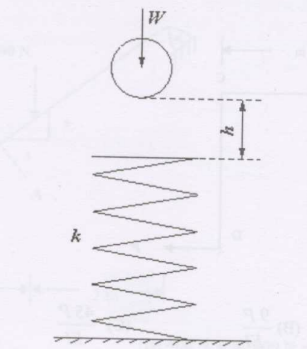
\includegraphics[width=0.5\columnwidth]{figs/ass1_f_q20.png}
    \caption{}
    \end{figure}

\begin{enumerate}
\begin{multicols}{4}
    \item  2.45 cm  
    \item  14.07 cm  
    \item  16.75 cm  
    \item  33 cm  
\end{multicols}
\end{enumerate}
    
    (GATE XE 2008)  

    \item A bullet of mass $m_{1} = 20\ \mathrm{gm}$ fired horizontally with a velocity of $v = 200\ \mathrm{m/s}$ hits a wooden block of mass $m_{2} = 500\ \mathrm{gm}$ (take $g = 9.8\ \mathrm{m/s^{2}}$) resting on a horizontal plane as shown in the figure and the bullet remains embedded in the block after the impact. If the coefficient of friction between the surfaces in contact remains constant at $0.3$, the distance the block will move before coming to rest is 

    \begin{figure}[H]
    \centering
    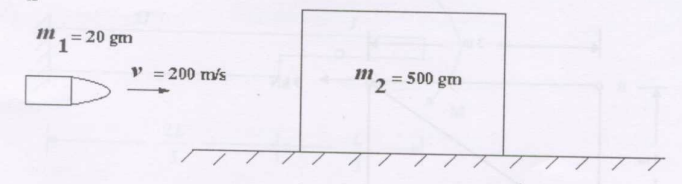
\includegraphics[width=0.7\columnwidth]{figs/ass1_f_q21.png}
    \caption{}
    \end{figure}

\begin{enumerate}
\begin{multicols}{4}
    \item  5.03 m  
    \item  10.06 m  
    \item  20.12 m  
    \item  100 m  
\end{multicols}
\end{enumerate}
    
    (GATE XE 2008)  

    \item A block of weight $500\ \mathrm{N}$ is about to move up the plane due to a horizontal force of $800\ \mathrm{N}$. The coefficient of static friction between the contact surfaces is 

    \begin{figure}[H]
    \centering
    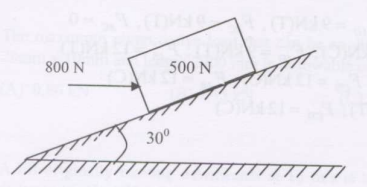
\includegraphics[width=0.5\columnwidth]{figs/ass1_f_q22.png}
    \caption{}
    \end{figure}

\begin{enumerate}
\begin{multicols}{4}
    \item  0.15  
    \item  0.25 
    \item  0.33  
    \item  0.53  
\end{multicols}
\end{enumerate}
    
    (GATE XE 2008)  


    \item The horizontal displacement at D of the frame shown in figure is (neglect axial strain energy and assume $EI$ to be constant throughout) 

    \begin{figure}[H]
    \centering
    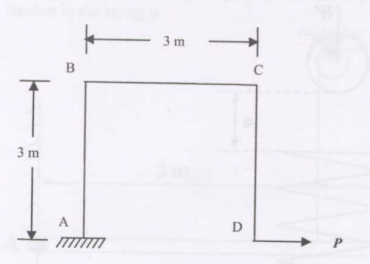
\includegraphics[width=0.5\columnwidth]{figs/ass1_f_q23.png}
    \caption{}
    \end{figure}

\begin{enumerate}
\begin{multicols}{4}
    \item  $\frac{6P}{EI}$ 
    \item  $\frac{9P}{EI}$ 
    \item  $\frac{45P}{EI}$ 
    \item  $\frac{729P}{EI}$ 
\end{multicols}
\end{enumerate}
    
    (GATE XE 2008)  

    \item The forces in the members of a truss ABCD as shown in the figure are (T stands for tension and C for compression)  

    \begin{figure}[H]
    \centering
    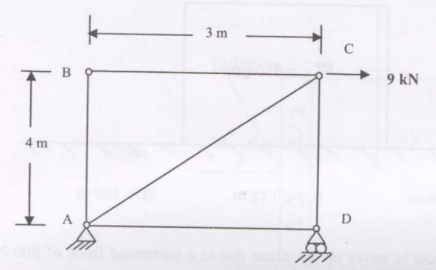
\includegraphics[width=0.5\columnwidth]{figs/ass1_f_q24.png}
    \caption{}
    \end{figure}

\begin{enumerate}

    \item  $F_{AB} = 12\ \mathrm{kN}(\mathrm{T}),\ F_{CD} = 12\ \mathrm{kN}(\mathrm{C}),\ F_{AD} = 9\ \mathrm{kN}(\mathrm{T}),\ F_{BC} = 9\ \mathrm{kN}(\mathrm{T}),\ F_{AC} = 0$  

    \item  $F_{BC} = 0,\ F_{AC} = 15\ \mathrm{kN}(\mathrm{T}),\ F_{CD} = 12\ \mathrm{kN}(\mathrm{C}),\ F_{AD} = 9\ \mathrm{kN}(\mathrm{T}),\ F_{AB} = 12\ \mathrm{kN}(\mathrm{T})$  

    \item  $F_{BC} = 0,\ F_{AC} = 15\ \mathrm{kN}(\mathrm{T}),\ F_{CD} = 12\ \mathrm{kN}(\mathrm{C}),\ F_{AB} = 12\ \mathrm{kN}(\mathrm{C})$  

    \item  $F_{AB} = F_{BC} = F_{AD} = 0,\ F_{AC} = 15\ \mathrm{kN}(\mathrm{T}),\ F_{CD} = 12\ \mathrm{kN}(\mathrm{C})$
\end{enumerate}    
    
    (GATE XE 2008)  

    \item The axial force, shear force and bending moment at section A-A of beam shown in figure are respectively  

    \begin{figure}[H]
    \centering
    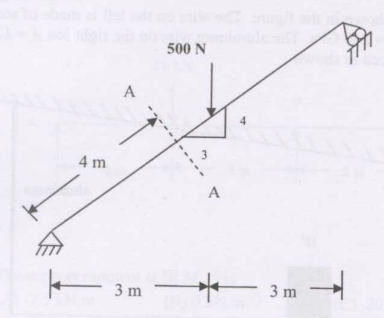
\includegraphics[width=0.5\columnwidth]{figs/ass1_f_q25.png}
    \caption{}
    \end{figure}

\begin{enumerate}
\begin{multicols}{2}
    \item  $-400\ \mathrm{N},\ 150\ \mathrm{N},\ 600\ \mathrm{N \cdot m}$  
    \item  $400\ \mathrm{N},\ 0,\ 600\ \mathrm{N \cdot m}$  
    \item  $0,\ 250\ \mathrm{N},\ 1000\ \mathrm{N \cdot m}$  
    \item  $-400\ \mathrm{N},\ 310\ \mathrm{N},\ 1240\ \mathrm{N \cdot m}$ 
\end{multicols}
\end{enumerate}
    
    (GATE XE 2008)  
    
    \item The slope and deflection at the free end of a variable cross section cantilever beam subjected to a bending moment at the free end as shown in the figure is  

    \begin{figure}[H]
    \centering
    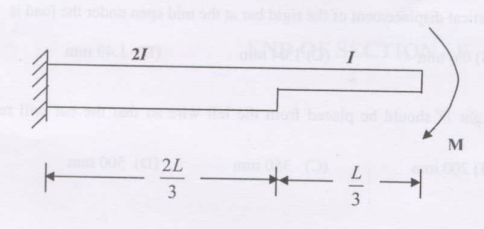
\includegraphics[width=0.5\columnwidth]{figs/ass1_d_q26.png}
    \caption{}
    \end{figure}

\begin{enumerate}
\begin{multicols}{4}    
    \item  $\dfrac{2ML}{3EI},\ \dfrac{5ML^2}{18EI}$  
    \item  $\dfrac{ML}{EI},\ \dfrac{ML^2}{2EI}$  
    \item  $\dfrac{ML}{1.5EI},\ \dfrac{ML^2}{3EI}$  
    \item  $\dfrac{ML}{3EI},\ \dfrac{ML^2}{3EI}$
\end{multicols}
\end{enumerate}
    
    (GATE XE 2008)  
    
    \item The maximum compressive load that can be applied on a hinged-hinged column of cross-section $20\ \mathrm{mm} \times 10\ \mathrm{mm}$ and length $2000\ \mathrm{mm}$ is (allowable compressive stress = $250\ \mathrm{MPa}$; $E = 210\ \mathrm{GPa}$)  

\begin{enumerate}
\begin{multicols}{4}    
    \item  $0.86\ \mathrm{kN}$  
    \item  $3.45\ \mathrm{kN}$  
    \item  $25\ \mathrm{kN}$  
    \item  $50\ \mathrm{kN}$ 
\end{multicols}
\end{enumerate}
    
    (GATE XE 2008)  
    
    \item A lift originally moving downwards at $10\ \mathrm{m/s}$ is brought to rest with a constant retardation in a distance of $25\ \mathrm{m}$. The force with which the feet of a passenger of mass $80\ \mathrm{kg}$ (take $g = 9.8\ \mathrm{m/s^2}$) press downwards on the floor of the lift is 

\begin{enumerate}
\begin{multicols}{4}
    \item  $160\ \mathrm{N}$  
    \item  $784\ \mathrm{N}$  
    \item  $944\ \mathrm{N}$  
    \item  $1000\ \mathrm{N}$ 
\end{multicols}
\end{enumerate}
    
    (GATE XE 2008)  

\item[] \textbf{\Large Common Data Questions}

\textbf{Common Data for Questions 29 and 30}

Two wires are connected to a rigid bar as shown in the figure. The wire on the left is made of steel having an area of cross section $A = 60 mm^2$ and $E = 210 GPa$. The aluminum wire on the right has $A = 120 m^2$ and $E = 70 GPa$. The weight $W = 100 kN$ is placed as shown

    \begin{figure}[H]
    \centering
    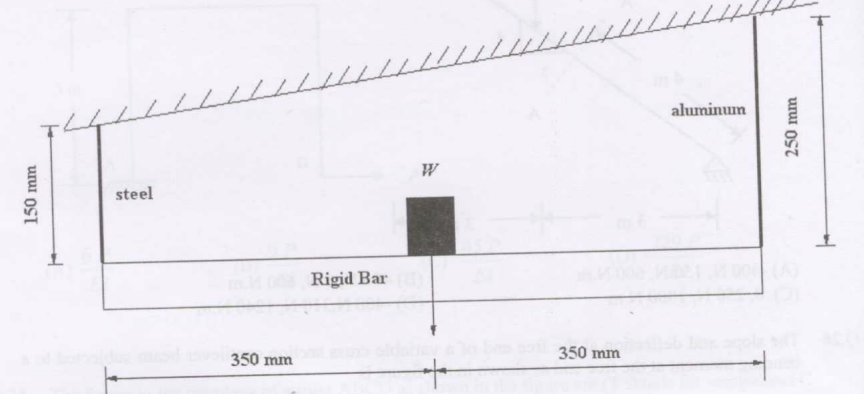
\includegraphics[width=0.7\columnwidth]{figs/ass1_f_q29.png}
    \caption{}
    \end{figure}


\item Due to this loading, the vertical displacement of the rigid bar at the mid span under the load is  

\begin{enumerate}
\begin{multicols}{4}
\item  $0.45 \ \mathrm{mm}$ \quad
\item  $0.6 \ \mathrm{mm}$ \quad
\item  $1.04 \ \mathrm{mm}$ \quad
\item  $1.49 \ \mathrm{mm}$ 
\end{multicols}
\end{enumerate}

(GATE XE 2008)

\item At what distance the weight $W$ should be placed from the left wire so that the bar will remain horizontal  

\begin{enumerate}
\begin{multicols}{4}
\item  $100 \ \mathrm{mm}$ \quad
\item  $200 \ \mathrm{mm}$ \quad
\item  $350 \ \mathrm{mm}$ \quad
\item  $500 \ \mathrm{mm}$  
\end{multicols}
\end{enumerate}

(GATE XE 2008)

\item[] \textbf{\Large Linked Answer Questions: Q.31 to Q.34 carry two marks each.}

\textbf{Statement for Linked Answer Questions 31 and 32:}

One end of a linear spring is attached to a fixed support and a mass of $2 kg$ hangs from it at the other end. A force of $4 N$ causes a displacement of $0.02m$. The mass is pulled down a distance of $0.04 m$ from its static equilibrium position and released with zero velocity


\item The natural frequency of vibration is  

\begin{enumerate}
\begin{multicols}{4}
\item  $1 \ \mathrm{rad/s}$ \quad
\item  $1.59 \ \mathrm{rad/s}$ \quad
\item  $5 \ \mathrm{rad/s}$ \quad
\item  $10 \ \mathrm{rad/s}$ 
\end{multicols}
\end{enumerate}

(GATE XE 2008)

\item The magnitude of velocity when the body has moved half way towards the static equilibrium position from its initial position is  

\begin{enumerate}
\begin{multicols}{4}
\item  $0.212 \ \mathrm{m/s}$ \quad
\item  $0.346 \ \mathrm{m/s}$ \quad
\item  $0.4 \ \mathrm{m/s}$ \quad
\item  $1.0 \ \mathrm{m/s}$
\end{multicols}
\end{enumerate}

(GATE XE 2008)

\item[] \textbf{Statement for Linked Answer Questions 33 and 34:}  

A two span variable cross section simply supported beam ABC is carrying two concentrated loads as shown in the figure.

    \begin{figure}[H]
    \centering
    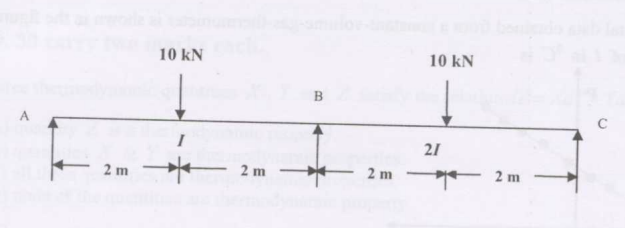
\includegraphics[width=0.7\columnwidth]{figs/ass1_f_q33.png}
    \caption{}
    \end{figure}

\item The support moment at $B$ ($M_B$) is  

\begin{enumerate}
\begin{multicols}{4}
\item  $-7.5\ \mathrm{kN \cdot m}$ \quad
\item  $0\ \mathrm{kN \cdot m}$ \quad
\item  $20\ \mathrm{kN \cdot m}$ \quad
\item  $80\ \mathrm{kN \cdot m}$ 
\end{multicols}
\end{enumerate}

(GATE XE 2008)


\item The support reactions are  

\begin{enumerate}
\begin{multicols}{4}
\item  $R_A = R_C = 3.125\ \mathrm{kN},\quad R_B = 13.75\ \mathrm{kN}$ \quad
\item  $R_A = R_C = R_B = 6.67\ \mathrm{kN}$ \quad
\item  $R_A = R_C = 5\ \mathrm{kN},\quad R_B = 10\ \mathrm{kN}$ \quad
\item  $R_A = R_C = 10\ \mathrm{kN},\quad R_B = 0$ 
\end{multicols}
\end{enumerate}

(GATE XE 2008)


\end{enumerate}

\begin{center}
    \textbf{END OF SECTION - F}
\end{center}

\newpage

\begin{center}
    \textbf{\Large G : THERMODYNAMICS}
\end{center}

\begin{enumerate}
\item[] \textbf{Q1 - Q8 carry one mark each}

\item Experimental data obtained from a constant-volume gas thermometer is shown in the figure below. The value of $t$ in $^\circ$C is  

    \begin{figure}[H]
    \centering
    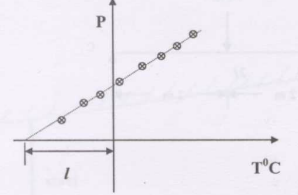
\includegraphics[width=0.5\columnwidth]{figs/ass1_g_q1.png}
    \caption{}
    \end{figure}
\begin{enumerate}
\begin{multicols}{4}
\item  $273.15$ \quad
\item  $1.0$ \quad
\item  $-100$ \quad
\item  $-273.15$  
\end{multicols}
\end{enumerate}

(GATE XE 2008)

\item At constant temperature, pressure of an incompressible fluid is changed from $400\ \mathrm{kPa}$ to $4\ \mathrm{MPa}$. Which of the following set of thermodynamic properties remain unchanged during the process: ($u$ is specific internal energy, $v$ is specific volume, $h$ is specific enthalpy and $s$ is specific entropy)  

\begin{enumerate}
\begin{multicols}{4}
\item  $u, v, h$ 
\item  $u, s, h$ 
\item  $u, v, s$ 
\item  $v, s, h$  
\end{multicols}
\end{enumerate}

(GATE XE 2008)

\item The densities of water and ice at $0^\circ$C are $1000\ \mathrm{kg/m^3}$ and $900\ \mathrm{kg/m^3}$, respectively. If ice at $0^\circ$C is allowed to melt into water at the same temperature, then  

\begin{enumerate}
\item  work is done by ice on the surrounding atmosphere. 
\item  work is done by the atmosphere on ice. 
\item  there is no work interaction. 
\item  nothing can be said about the work interaction.  
\end{enumerate}

(GATE XE 2008)

\item The work done in an isentropic process involving ideal gas is equal to  

\begin{enumerate}
\begin{multicols}{2}
\item  $-\int V\, dP$ \quad
\item  Zero \quad
\item  $\dfrac{P_1 V_1 - P_2 V_2}{\gamma - 1}$ \quad
\item  $RT \ln \left( \dfrac{V_2}{V_1} \right)$  
\end{multicols}
\end{enumerate}

(GATE XE 2008)

\item Thermal efficiency of a Diesel cycle can be increased by  

\begin{enumerate}
\item  increasing both compression ratio and cut-off ratio. 
\item  decreasing both compression ratio and cut-off ratio. 
\item  decreasing compression ratio and increasing cut-off ratio. 
\item  increasing compression ratio and decreasing cut-off ratio.  
\end{enumerate}

(GATE XE 2008)

\item In a throttling process  

\begin{enumerate}
\item  temperature always remains unchanged.
\item  temperature always increases.
\item  temperature always decreases.
\item  temperature may increase, decrease or remain unchanged.  
\end{enumerate}
(GATE XE 2008)

\item The COP of a Carnot heat pump operating between $-3^\circ\mathrm{C}$ and $27^\circ\mathrm{C}$ is  

\begin{enumerate}
\begin{multicols}{4}
\item  $10$ 
\item  $0.1$ 
\item  $9.0$ 
\item  $1.0$  
\end{multicols}
\end{enumerate}

(GATE XE 2008)

\item If the moist air is heated at a constant pressure  

\begin{enumerate}
\begin{multicols}{2}
\item  the specific humidity changes.
\item  the relative humidity does not \newline change.
\item  the relative humidity decreases.
\item  the relative humidity increases.
\end{multicols}
\end{enumerate}

(GATE XE 2008)

\item[] \textbf{Q. 9 to Q. 30 carry two marks each.}

\item Three thermodynamic quantities $X, Y$ and $Z$ satisfy the relation  
$dZ = X\, dY + Y\, dX.$
This implies,  
\begin{enumerate}
\item  quantity $Z$ is a thermodynamic property.
\item  quantities $X$ and $Y$ are thermodynamic properties. 
\item  all three quantities are thermodynamic properties. 
\item  none of the quantities are thermodynamic property. 
\end{enumerate}

(GATE XE 2008)

\item In a constant temperature process 70 moles of an ideal gas at temperature $354\ \mathrm{K}$ attains a final volume $V_2 = 1\ \mathrm{m^3}$. Work input during this process is $206\ \mathrm{kJ}$. Initial volume $V_1$ of the gas approximately satisfies the following relation ($e$ is the base of natural logarithm)  

\begin{enumerate}
\begin{multicols}{4}
\item  $V_1 = V_2$ 
\item  $V_1 = e\,V_2$ 
\item  $\ln \left( \dfrac{V_2}{V_1} \right) = 1$ 
\item  $V_1 = \ln (V_2)$ 
\end{multicols}
\end{enumerate}

(GATE XE 2008)

\item An ideal gas at pressure $P_0$ and temperature $T_0$ undergoes a reversible isothermal compression and attains a pressure $P_1$. The characteristic gas constant is $R$. Net heat transferred during this process is  

\begin{enumerate}
\begin{multicols}{4}
\item  zero 
\item  $RT_0 \ln\left( \dfrac{P_1}{P_0} \right)$ 
\item  $-RT_0 \ln\left( \dfrac{P_1}{P_0} \right)$ 
\item  $RT_0 \dfrac{(P_0 - P_1)}{P_0}$  
\end{multicols}
\end{enumerate}

(GATE XE 2008)

\item A person starts a $60\ \mathrm{W}$ table fan in an insulated room of volume $30.4\ \mathrm{m^3}$. The person expects to cool the room from $32^\circ\mathrm{C}$ (pressure = $100\ \mathrm{kPa}$) and allows the fan to rotate for $4$ hours. If the specific heat at constant volume of the room air is $0.718\ \mathrm{kJ/(kg\ K)}$ and characteristic gas constant is $287\ \mathrm{J/(kg\ K)}$, after 4 hours, the person will find that the room is  

\begin{enumerate}
\item  hotter by approximately $12^\circ$C.
\item  cooler by approximately $10^\circ$C.
\item  at the same temperature.
\item  hotter by approximately $8^\circ$C.
\end{enumerate}

(GATE XE 2008)

\item Consider the cycles given below and state which one of the following statements is true

    \begin{figure}[H]
    \centering
    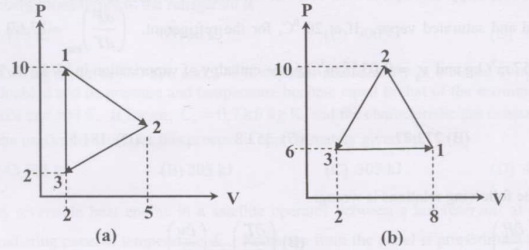
\includegraphics[width=0.5\columnwidth]{figs/ass1_g_q13.png}
    \caption{}
    \end{figure}

\begin{enumerate}
\item  In both (a) and (b) net work done is $+12$ units.
\item  In (b) net work done is more since in (a) no work is produced by the constant volume process.
\item  Magnitudes of net work produced in both (a) and (b) are $12$ units but their signs are opposite.
\item  Magnitudes of net work produced in both (a) and (b) are different.  
\end{enumerate}

(GATE XE 2008)

\item Steam of quality $0.98$ is present in two separate containers A and B at $300\ \mathrm{kPa}$ and $200\ \mathrm{kPa}$, respectively. Specific volumes of steam in containers A and B initially are $v_A$ and $v_B$, respectively. Steam condenses at a constant pressure in such a way that the final quality of steam in both the containers is $0.01$ and specific volumes of steam in containers A and B are $v_{A2}$ and $v_{B2}$, respectively. Which one of the following statements is true?  

\begin{enumerate}
\item  $v_A > v_{A2}$ and $v_{B2} > v_B$  
\item  $v_A < v_{A2}$ and $v_{B2} < v_B$  
\item  $v_A > v_{A2}$ and $v_{B2} < v_B$  
\item  $v_A < v_{A2}$ and $v_{B2} > v_B$  
\end{enumerate}

(GATE XE 2008)

\item The approximate entropy change, when $10\ \mathrm{kg}$ of an ideal gas having specific heat at constant volume $c_v = \dfrac{5R}{2}$ (given, $R = 287\ \mathrm{J/(kg\ K)}$) is taken from an initial state of $100\ \mathrm{kPa}$ and $300\ \mathrm{K}$ to the final state of $200\ \mathrm{kPa}$ and $500\ \mathrm{K}$, is  

\begin{enumerate}
\begin{multicols}{4}
\item  $9.1$  
\item  $3.14$  
\item  $91.0$  
\item  $0.314$ 
\end{multicols}
\end{enumerate}

(GATE XE 2008)

\item In a thermal power plant operating on a Rankine cycle, steam having enthalpy $h = 2995.1\ \mathrm{kJ/kg}$ and entropy $s = 6.5422\ \mathrm{kJ/(kg\ ^\circ C)}$ is produced at $3\ \mathrm{MPa}$ and $300\ ^\circ \mathrm{C}$ and is fed to a turbine where it expands to a condenser pressure of $5\ \mathrm{kPa}$. The dryness fraction of steam at the exit of the turbine is $x_t = 0.9761$ and $s_f = 0.4763\ \mathrm{kJ/(kg\ ^\circ C)}$ and $s_g = 8.3960\ \mathrm{kJ/(kg\ ^\circ C)}$. At the entrance to the condenser, the quality and enthalpy of steam, respectively, are approximately:  

\begin{enumerate}
\begin{multicols}{4}
\item  $0.89,\ 1994.42$  
\item  $0.68,\ 1795.67$  
\item  $0.79,\ 2055.02$  
\item  $0.77,\ 2004.12$  
\end{multicols}
\end{enumerate}

(GATE XE 2008)

\item For a refrigerant, the slope $\left( \dfrac{dP}{dT} \right)_{\mathrm{sat}}$ of the saturation curve on a $P$–$T$ diagram is a function of the temperature, the enthalpy of vaporization and the difference between specific volumes of the saturated liquid and saturated vapor. If at $20\ ^\circ\mathrm{C}$, for the refrigerant, $\left( \dfrac{dP}{dT} \right)_{\mathrm{sat}} = 17.69\ \mathrm{kPa/K}$, $v_f = 0.0008157\ \mathrm{m^3/kg}$ and $v_g = 0.0358\ \mathrm{m^3/kg}$, the enthalpy of vaporization in $\mathrm{kJ/kg}$ at $20\ ^\circ\mathrm{C}$ is approximately:  

\begin{enumerate}
\begin{multicols}{4}
\item  $12.38$  
\item  $273.77$  
\item  $353.8$  
\item  $181.5$  
\end{multicols}
\end{enumerate}

(GATE XE 2008)

\item Which one of the following relations is wrong:  

\begin{enumerate}
\begin{multicols}{2}
\item  $\left( \frac{\partial T}{\partial v} \right)_s = -\left( \frac{\partial P}{\partial s} \right)_v$  
\item  $\left( \frac{\partial T}{\partial P} \right)_s = \left( \frac{\partial v}{\partial s} \right)_P$  
\item  $\left( \frac{\partial P}{\partial T} \right)_v = \left( \frac{\partial s}{\partial v} \right)_T$  
\item  $\left( \frac{\partial s}{\partial P} \right)_T = -\left( \frac{\partial v}{\partial T} \right)_P$  
\end{multicols}
\end{enumerate}

(GATE XE 2008)

\item  For the same maximum temperature and pressure, an Otto cycle and a Diesel cycle are shown on the same T-s diagram in the following figure. Which one of the following is correct:  

    \begin{figure}[H]
    \centering
    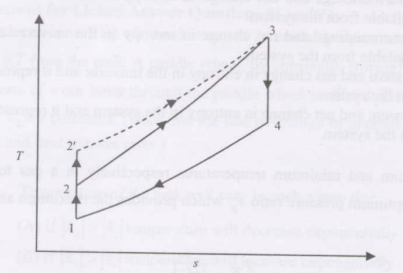
\includegraphics[width=0.5\columnwidth]{figs/ass1_g_q19.png}
    \caption{}
    \end{figure}
\begin{enumerate}
\item  1-2-3-4 is an Otto cycle and 2-3 is an isobaric process. 
\item  1-2-3-4 is an Otto cycle and 2$'$-3 is an isobaric process. 
\item  1-2-3-4 is an Otto cycle and 2-3 is an isochoric process. 
\item  1-2-3-4 is a Diesel cycle and 2$'$-3 is an isochoric process.
\end{enumerate}

(GATE XE 2008)

\item  A Carnot engine having efficiency $\eta = 0.5$ drives a Carnot refrigerator with COP = 4. The energy absorbed by the refrigerator from the cold body for each kJ of energy absorbed from the source by the Carnot engine is  

\begin{enumerate}
\begin{multicols}{4}
\item  $ 2 kJ$  
\item  $2.4 kJ $ 
\item  $3 kJ$  
\item  $4 kJ$  
\end{multicols}
\end{enumerate}

(GATE XE 2008)

\item  It is proposed that the solar energy be used to heat a large collector plate. The engine in turn transfers heat to a fluid within a heat engine, and the engine would reject energy as heat to the atmosphere. Experiments indicate that 0.5 kW/m$^2$ of energy can be collected at the operating temperature of the plate and the maximum efficiency of the engine is 0.2. The minimum collector area that would be required for a plant to produce 1 kW of useful shaft power is  

\begin{enumerate}
\begin{multicols}{4}
\item  1 m$^2$  
\item  10 m$^2$ 
\item  100 m$^2$  
\item  1000 m$^2$  
\end{multicols}
\end{enumerate}

(GATE XE 2008)

\item  A reversible engine operates between temperatures $T_1 = 1000 \, \mathrm{K}$ and $T_2 = 400 \, \mathrm{K}$. The engine drives a refrigerator which operates between $T_2 = 400 \, \mathrm{K}$ and $T_3 = 200 \, \mathrm{K}$. The energy transfer to the engine is 2000 kJ and the net work output of the combined engine and refrigerator is 300 kJ. The energy transferred to the refrigerant is  

\begin{enumerate}
\begin{multicols}{4}
\item  $9 kJ$  
\item  $90 kJ$  
\item  $900 kJ$  
\item  $9000 kJ$  
\end{multicols}
\end{enumerate}
(GATE XE 2008)

\item  Two kg of air at 500 kPa and 370 K expands adiabatically in a closed system until its volume is doubled and its pressure and temperature become equal to that of the surroundings, which is at 100 kPa and 300 K. If for air, $C_v = 0.7 \, \mathrm{kJ/kg \cdot K}$ and the characteristic gas constant $R = 0.287 \, \mathrm{kJ/kg \cdot K}$, the maximum work for this process is approximately given by

\begin{enumerate}
\begin{multicols}{4}
\item  $105 kJ$  
\item  $205 kJ$  
\item  $305 kJ$  
\item  $405 kJ$  
\end{multicols}
\end{enumerate}

(GATE XE 2008)

\item  A reversible heat engine in a satellite operates between a hot reservoir at temperature $T_r$ and a radiating panel at temperature $T_p$. Radiation from the panel is proportional to the area $A$ and $T_p^4$. The constant of proportionality is the Stefan–Boltzmann constant $\sigma$. The ratio of the work output $W$ to the temperature difference $(T_r - T_p)$ is  

\begin{enumerate}
\begin{multicols}{4}
\item  $\sigma A T$  
\item  $\sigma A T^2$  
\item  $\sigma A T_p^2$  
\item  $\sigma A T_p^4$ 
\end{multicols}
\end{enumerate}

(GATE XE 2008)

\item Irreversibility of a given process in a system is equal to  

\begin{enumerate}
\item  product of temperature of the surroundings and net change in entropy in the universe and it represents loss in total work available from the system.  
 \item  product of temperature of the surroundings and net change in entropy in the universe and it represents gain in total work available from the system.  
 \item  product of temperature of the system and net change in entropy in the universe and it represents loss in total work available from the system. 
  \item  product of temperature of the system and net change in entropy in the system and it represents loss in total work available from the system.
 \end{enumerate}
 
 (GATE XE 2008)  

\item $T_{\max}$ and $T_{\min}$ represent the maximum and minimum temperatures respectively in a gas turbine working on a Brayton cycle. The optimum pressure ratio $r_p$ which provides the maximum amount of work is given by  

\begin{enumerate}
\begin{multicols}{2}
\item  $r_p = \left( \frac{T_{\max}}{T_{\min}} \right)^{\frac{2\gamma - 1}{\gamma}}$
\item $r_p = \left( \frac{T_{\max}}{T_{\min}} \right)^{\frac{\gamma}{2\gamma -1}}$
\item $r_p = \left( \frac{T_{\min}}{T_{\max}} \right)^{\frac{\gamma}{2\gamma-1}}$
\item $ r_p = \left( \frac{T_{\min}}{T_{\max}} \right)^{\frac{2\gamma - 1}{\gamma}}$
\end{multicols}
\end{enumerate}


 (GATE XE 2008)  

\item A heat engine operates between three reservoirs: $R_1$ at 550 K, $R_2$ at 450 K and $R_3$ at 350 K. For every cycle, the engine accepts 100 kJ from $R_1$ and rejects 60 kJ into $R_2$ and 30 kJ into $R_3$. The engine efficiency is  

\begin{enumerate}
\begin{multicols}{4}
 \item  0.10  
 \item  0.20  
 \item  0.30  
 \item  can not be defined  
 \end{multicols}
 \end{enumerate}

 (GATE XE 2008)  

\item Carbon tetrachloride boils at $76^{\circ}$C at 101 kPa. The latent heat of vaporization of carbon tetrachloride is 195 kJ/kg and for this, the characteristic gas constant is 0.055 kJ/kg K. The boiling point of carbon tetrachloride at 202 kPa is 

\begin{enumerate}
\begin{multicols}{4}
 \item  274.54 K  
 \item  374.54 K  
 \item  474.54 K  
 \item  574.54 K  
 \end{multicols}
 \end{enumerate}

(GATE XE 2008)  


\item[] \textbf{\Large Common Data Questions}

\textbf{Common Data for Questions 29 and 30:}  

Steam at 0.6181 MPa and 160$^\circ$C (saturated) enters a steady flow device with a velocity of 50 m/s and enthalpy 2756.7 kJ/kg. It leaves at a pressure of 0.1 MPa with a velocity of 600 m/s and enthalpy $h_2$. The device is perfectly insulated and does not do any work on the surroundings. Neither does it receive any work input. Use the following data table:  

\begin{table}[H]     \centering     \caption{}     \label{}     \begin{tabular}{|c|c|c|c|c|c|}
\hline
\multirow{2}{*}{\textbf{Pressure} $P$ (bar)} & 
\multirow{2}{*}{\textbf{Temperature} ($^{\circ}$C)} & 
\multicolumn{2}{c|}{\textbf{Specific enthalpy}} & 
\multicolumn{2}{c|}{\textbf{Specific entropy}} \\ \cline{3-6}
 & & $h_f$ (kJ/kg) & $h_g$ (kJ/kg) & $s_f$ (kJ/kgK) & $s_g$ (kJ/kgK) \\ \hline
1.5 & 111.37 & 467.13 & 2693.4 & 1.4336 & 7.2234 \\ \hline
\end{tabular} \end{table}


\item The quality of the steam at the outlet of the device is  
\begin{enumerate}
\begin{multicols}{4}
\item  0.548  
\item  0.648  
\item  0.748  
\item  0.948  
\end{multicols}
\end{enumerate}

 (GATE XE 2008)  

\item The above mentioned device is a  

\begin{enumerate}
\begin{multicols}{4}
 \item  turbine  
 \item  compressor  
 \item  nozzle  
 \item  diffuser 
\end{multicols}
\end{enumerate}

 (GATE XE 2008)  

\item[] \textbf{\Large Linked Answer Questions: Q.31 to Q.34 carry two marks each.}

\textbf{Statement for Linked Answer Questions 31 and 32:}  

A tank contains $9~\mathrm{kg}$ of liquid water at an initial temperature $T_0~^{\circ}\mathrm{C}$.  
A coil removes heat at the rate of $\dot{Q} = k_1 T$ from the tank. A paddle wheel, by constantly stirring, maintains uniform temperature in the tank.  
The rate of work input through the paddle wheel is $\dot{W} = k_2 T$. Temperature, $T$ is in $^{\circ}\mathrm{C}$ and $k_1$ and $k_2$ are constants.  
(Note that the rate of change in internal energy inside the tank will be a balance of work and heat transfer rates.)  

\item Temperature of the tank will vary in such a way that  

\begin{enumerate}
\item  If $|k_2| > |k_1|$ temperature will decrease exponentially  
\item  If $|k_2| > |k_1|$ temperature will increase exponentially  
\item  If $|k_2| < |k_1|$ temperature will increase exponentially  
\item  If $|k_2| > |k_1|$ temperature will decrease linearly  
\end{enumerate}

(GATE XE 2008)  

\item If $T_0 = 80\,^{\circ}\mathrm{C}$, $|k_1| = 0.1$, $|k_2| = 0.01$ and specific heat of the liquid $= 1.0$, the temperature of the tank after $1~\mathrm{minute}$ will be  

\begin{enumerate}
\begin{multicols}{4}
\item  $43.9^{\circ}\mathrm{C}$ 
\item  $38.4^{\circ}\mathrm{C}$ 
\item  $166.6^{\circ}\mathrm{C}$ 
\item  $145.7^{\circ}\mathrm{C}$ 
\end{multicols}
\end{enumerate}

(GATE XE 2008)  

\item[] \textbf{Statement for Linked Answer Questions 33 and 34:}  

Air enters a gas turbine at $1.0135~\mathrm{MPa}$, $1000~\mathrm{K}$ at the rate of $1~\mathrm{kg/s}$ and exits at $101.35~\mathrm{kPa}$ and $600~\mathrm{K}$.  
Neglect the changes in potential energy and kinetic energy and assume that air is an ideal gas with $R = 0.287~\mathrm{kJ/(kg\,K)}$, $c_p = 1.005~\mathrm{kJ/(kg\,K)}$.  

\item The net power output of the gas turbine is 

\begin{enumerate}
\begin{multicols}{4}
\item  $102~\mathrm{kW}$ 
\item  $200~\mathrm{kW}$ 
\item  $301~\mathrm{kW}$ 
\item  $402~\mathrm{kW}$  
\end{multicols}
\end{enumerate}

(GATE XE 2008)  

\item If for the isentropic process  
$
\frac{T_2}{T_1} = \left( \frac{P_2}{P_1} \right)^{\frac{\gamma-1}{\gamma}}
$ 
and $\gamma = 1.4$, the isentropic efficiency of the turbine is  

\begin{enumerate}
\begin{multicols}{4}
\item  $63\%$ 
\item  $73\%$ 
\item  $83\%$
\item  $93\%$  
\end{multicols}
\end{enumerate}

(GATE XE 2008)  

\end{enumerate}

\begin{center}
    \textbf{END OF SECTION - G}
\end{center}

\newpage

\begin{center}
    \textbf{\Large H : POLYMER SCIENCE AND ENGINEERING}
\end{center}

\begin{enumerate}
\item[] \textbf{Q1 - Q8 carry one mark each}

\item Among the polymerization methods listed below, the one that is likely to give a polydispersity close to unity is  

\begin{enumerate}
\begin{multicols}{2}
\item  Anionic polymerization  
\item  Cationic polymerization  
\item  Condensation polymerization  
\item  Radical polymerization  
\end{multicols}
\end{enumerate}

 (GATE XE 2008)

\item The end-groups in a polymer sample prepared by using $\mathrm{ROOH}/\mathrm{Fe}^{2+}$ (where R = alkyl) as the initiator system is  

\begin{enumerate}
\begin{multicols}{4}
\item  $\mathrm{Fe}^{2+}$  
\item  $- \mathrm{OR}$  
\item  $- \mathrm{OH}$  
\item  $\mathrm{Fe}^{3+}$ 
\end{multicols}
\end{enumerate}

 (GATE XE 2008)

\item Most polymers exhibit Newtonian behaviour at  

\begin{enumerate}
\begin{multicols}{2}
\item  High temperature  
\item  Low shear rate  
\item  High molecular weight  
\item  Low filler content  
\end{multicols}
\end{enumerate}

(GATE XE 2008)

\item The shear rate of a typical injection molding process is  

\begin{enumerate}
\begin{multicols}{4}
\item  $1~\mathrm{s^{-1}}$  
\item  $10~\mathrm{s^{-1}}$  
\item  $100~\mathrm{s^{-1}}$  
\item  $1000~\mathrm{s^{-1}}$  
\end{multicols}
\end{enumerate}

(GATE XE 2008)

\item Which of the following monomers is used in the synthesis of poly(vinyl alcohol) is  

\begin{enumerate}
\begin{multicols}{4}
\item  $\mathrm{CH_3CH_2OH}$  
\item  $\mathrm{CH_2=CH(OH)}$  
\item  $\mathrm{CH_2=CH-O-CO-CH_3}$  
\item  $\mathrm{CH_2=CH-CO_2H}$  
\end{multicols}
\end{enumerate}

(GATE XE 2008)

\item The extension ratio of an elastomer deformed to $10$ times its original length is  

\begin{enumerate}
\begin{multicols}{4}
\item  $2$  
\item  $5$  
\item  $9$  
\item  $11$  
\end{multicols}
\end{enumerate}

(GATE XE 2008)

\item Most plausible value for the Gibbs free energy change for a miscible blend of two polymers is  

\begin{enumerate}
\begin{multicols}{4}
\item  $+5~\mathrm{kJ\,mol^{-1}}$  
\item  $+1~\mathrm{kJ\,mol^{-1}}$  
\item  $0~\mathrm{kJ\,mol^{-1}}$  
\item  $-0.01~\mathrm{kJ\,mol^{-1}}$  
\end{multicols}
\end{enumerate}

 (GATE XE 2008)

\item The glass transition temperature of raw natural rubber is  

\begin{enumerate}
\begin{multicols}{4}
\item  $-70\,^{\circ}\mathrm{C}$  
\item  $-10\,^{\circ}\mathrm{C}$  
\item  $0\,^{\circ}\mathrm{C}$  
\item  $+30\,^{\circ}\mathrm{C}$ 
\end{multicols}
\end{enumerate}

(GATE XE 2008)

\item[] \textbf{Q. 9 to Q.30 carry two marks each.}


\item $2,2'$-Azobisisobutyronitrile (AIBN) is an initiator used in the free radical polymerization of methyl methacrylate (MMA). When the concentration of AIBN is doubled maintaining MMA concentration unchanged, the rate of propagation  

\begin{enumerate}
\begin{multicols}{2}
\item  Is doubled  
\item  Increases by a factor of $\sqrt{2}$  
\item  Is reduced by half  
\item  Decreases by a factor of $\sqrt{2}$  
\end{multicols}
\end{enumerate}

(GATE XE 2008)

\item A polymer sample has $3$ molecules with molecular weights $1\times 10^5$, $2\times 10^5$ and $3\times 10^5~\mathrm{g\,mol^{-1}}$ respectively. The weight average molecular weight of the sample is  

\begin{enumerate}
\begin{multicols}{2}
\item  $2.99\times 10^5~\mathrm{g\,mol^{-1}}$  
\item  $2.66\times 10^5~\mathrm{g\,mol^{-1}}$  
\item  $2.33\times 10^5~\mathrm{g\,mol^{-1}}$  
\item  $2.00\times 10^5~\mathrm{g\,mol^{-1}}$ 
\end{multicols}
\end{enumerate}

 (GATE XE 2008)

\item Which of the following reagents is capable of effecting Group Transfer polymerization with methacrylates?  

\
\begin{multicols}{2}
 \begin{figure}[H]
    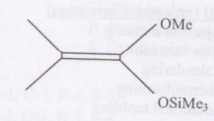
\includegraphics[width=0.4\columnwidth]{figs/ass1_h_q11_1.png}
    \caption{A}
    \end{figure}
    
  \begin{figure}[H]
    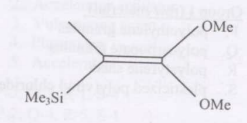
\includegraphics[width=0.4\columnwidth]{figs/ass1_h_q11_2.png}
    \caption{B}
    \end{figure}
 
  \begin{figure}[H]
    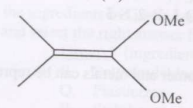
\includegraphics[width=0.4\columnwidth]{figs/ass1_h_q11_3.png}
    \caption{C}
    \end{figure}
    
  \begin{figure}[H]
    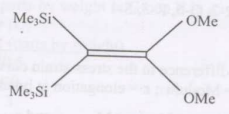
\includegraphics[width=0.4\columnwidth]{figs/ass1_h_q11_4.png}
    \caption{D}
    \end{figure}
\end{multicols}    


(GATE XE 2008)

\item For the copolymerization of MMA with vinyl chloride, the monomer reactivity ratios were found to be $10$ and $0.1$ respectively. The resulting polymer is most likely to be 

\begin{enumerate}
\begin{multicols}{2}
\item  an alternating copolymer  
\item  an ideal copolymer  
\item  a block copolymer  
\item  a branched copolymer  
\end{multicols}
\end{enumerate}

 (GATE XE 2008)

\item Match the characterization techniques listed in Group I with the applications listed in Group II and select the correct answer from (A), (B), (C) or (D):

\begin{table}[H]     \centering     \caption{}     \label{}     \begin{tabular}{ll}
\textbf{Group I (Technique)} & \textbf{Group II (Application)} \\
P. X-ray Diffraction & 1. Functional Groups \\
Q. Differential Thermal Analysis & 2. Crystallinity \\
R. Infrared Spectroscopy & 3. Morphology \\
S. Microscopy & 4. Enthalpy \\
 & 5. Power Factor \\
\end{tabular} \end{table}

\begin{enumerate}
\begin{multicols}{2}
\item  P-5, Q-4, R-3, S-2  
\item  P-2, Q-3, R-1, S-5  
\item  P-3, Q-2, R-4, S-5  
\item  P-2, Q-4, R-1, S-3  
\end{multicols}
\end{enumerate}

(GATE XE 2008)

\item For a polymer, viscosity at $50\,^{\circ}\mathrm{C}$ and at $80\,^{\circ}\mathrm{C}$ was found to be $2.00~\mathrm{Pa\cdot s}$ and $1.00~\mathrm{Pa\cdot s}$ respectively. The value of viscosity at $60\,^{\circ}\mathrm{C}$ is  

\begin{enumerate}
\begin{multicols}{4}
\item  $1.65~\mathrm{Pa\cdot s}$  
\item  $1.55~\mathrm{Pa\cdot s}$  
\item  $1.45~\mathrm{Pa\cdot s}$  
\item  $1.35~\mathrm{Pa\cdot s}$  
\end{multicols}
\end{enumerate}

 (GATE XE 2008)

\item For a viscoelastic material behaving as Maxwell model, the modulus at its relaxation time under constant strain reduces to  

\begin{enumerate}
\item  $36.8\%$ of the initial value  
\item  $63.2\%$ of the initial value  
\item  $66.7\%$ of the initial value  
\item  $50.0\%$ of the initial value 
\end{enumerate}

(GATE XE 2008)

\item The capacity of an extruder can be maximized by a combination of  

\begin{enumerate}
\item  higher barrel diameter; higher screw diameter; higher helix angle; higher rpm  
\item  higher barrel diameter; higher screw diameter; higher helix angle; lower rpm 
\item  higher barrel diameter; higher screw diameter; lower helix angle; higher rpm 
\item  higher barrel diameter; lower screw diameter; higher helix angle; higher rpm
\end{enumerate}

(GATE XE 2008)

\item Match the raw materials in Group I with the polymer processing operation in Group II and select the correct answer from (A), (B), (C) or (D).

\begin{table}[H]     \centering     \caption{}     \label{}     \begin{tabular}{l l}
\textbf{Group I (raw material)} & \textbf{Group II (processing operation)} \\
P. polyethylene granules & 1. Injection molding \\
Q. polycarbonate granules & 2. Film extrusion \\
R. polystyrene sheet & 3. Calendering \\
S. plasticized poly(vinyl chloride) & 4. Thermoforming \\
& 5. Rotational molding \\
\end{tabular} \end{table}

\begin{enumerate}
\begin{multicols}{2}
\item  P-1, Q-2, R-3, S-4 
\item  P-2, Q-1, R-4, S-3 
\item  P-2, Q-5, R-3, S-1 
\item  P-4, Q-3, R-2, S-5
\end{multicols}
\end{enumerate}

(GATE XE 2008)

\item The difference in the stress-strain curve for plastics, elastomer and metals can be represented by: \\
(M = Modulus; $\varepsilon$ = elongation at break)

\begin{enumerate}
\item  $M_{\text{metal}} < M_{\text{plastic}} < M_{\text{elastomer}}$ and $\varepsilon_{\text{metal}} \geq \varepsilon_{\text{plastic}} \geq \varepsilon_{\text{elastomer}}$ 
\item  $M_{\text{plastic}} < M_{\text{elastomer}} < M_{\text{metal}}$ and $\varepsilon_{\text{plastic}} \geq \varepsilon_{\text{elastomer}} \geq \varepsilon_{\text{metal}}$ 
\item  $M_{\text{elastomer}} < M_{\text{plastic}} < M_{\text{metal}}$ and $\varepsilon_{\text{elastomer}} \geq \varepsilon_{\text{plastic}} \geq \varepsilon_{\text{metal}}$ 
\item  $M_{\text{plastic}} > M_{\text{metal}} > M_{\text{elastomer}}$ and $\varepsilon_{\text{plastic}} \geq \varepsilon_{\text{metal}} \geq \varepsilon_{\text{elastomer}}$
\end{enumerate}

(GATE XE 2008)

\item Match the following rubbers in Group I with their applications in Group II and select the correct answer from (A), (B), (C) or (D).

\begin{table}[H]     \centering     \caption{}     \label{}     \begin{tabular}{l l}
\textbf{Group I (rubbers)} & \textbf{Group II (applications)} \\
P. Butyl rubber & 1. Gaskets in chemical plants \\
Q. Fluorocarbon elastomer & 2. Petrol hoses \\
R. Natural rubber & 3. Hand gloves \\
S. Nitrile rubber & 4. Roofing membrane \\
& 5. Tire inner liner \\
\end{tabular} \end{table}

\begin{enumerate}
\begin{multicols}{2}
\item  P-5, Q-1, R-3, S-2 
\item  P-1, Q-3, R-2, S-5 
\item  P-2, Q-3, R-1, S-4 
\item  P-3, Q-5, R-1, S-4
\end{multicols}
\end{enumerate}

(GATE XE 2008)

\item A carbon fiber-epoxy bar of dimensions ($0.5\,\mathrm{m} \times 0.04\,\mathrm{m} \times 0.04\,\mathrm{m}$) gave a breaking load of $784\,\mathrm{N}$ in a three point bending test. The flexural strength of the material is:

\begin{enumerate}
\begin{multicols}{4}
\item  $15.8\ \mathrm{MPa}$
\item  $9.2\ \mathrm{MPa}$ 
\item  $0.3\ \mathrm{GPa}$ 
\item  $108.1\ \mathrm{GPa}$
\end{multicols}
\end{enumerate}

(GATE XE 2008)

\item Match the polymers in Group I with their crystalline melting point ($m_p$, $^\circ$C) in Group II and select the correct answer from (A), (B), (C) or (D).

\begin{table}[H]     \centering     \caption{}     \label{}     \begin{tabular}{l l}
\textbf{Group I (polymers)} & \textbf{Group II ($m_p$, $^\circ$C)} \\
P. Nylon66 & 1. 108 \\
Q. PBT & 2. 320 \\
R. PP & 3. 264 \\
S. LDPE & 4. 165 \\
& 5. 220 \\
\end{tabular} \end{table}

\begin{enumerate}
\begin{multicols}{2}
\item  P-1, Q-3, R-5, S-2 
\item  P-3, Q-4, R-2, S-5 
\item  P-3, Q-5, R-4, S-1 
\item  P-5, Q-1, R-3, S-4
\end{multicols}
\end{enumerate}

(GATE XE 2008)

\item Match the additives listed in Group I below with their function listed in Group II and select the right answer from (A), (B), (C) or (D).

\begin{table}[H]     \centering     \caption{}     \label{}     \begin{tabular}{l l}
\textbf{Group I (additives)} & \textbf{Group II (function)} \\
P. Sulfur & 1. Age resistor \\
Q. Zinc oxide & 2. Accelerator activator \\
R. Paraphenylene diamine & 3. Vulcanizing agent \\
S. Dioctyl phthalate & 4. Plasticizer \\
& 5. Accelerator \\
\end{tabular} \end{table}

\begin{enumerate}
\begin{multicols}{2}
\item  $P$-1, $Q$-3, $R$-4, $S$-5 
\item  $P$-3, $Q$-2, $R$-1, $S$-4 
\item  $P$-2, $Q$-4, $R$-5, $S$-1 
\item  $P$-2, $Q$-4, $R$-5, $S$-1 
\end{multicols}
\end{enumerate}

(GATE XE 2008)

\item Match the ingredients in Group I with their amount in parts by weight in Group II in a typical recipe and select the right answer from (A), (B), (C) or (D).

\begin{table}[H]     \centering     \caption{}     \label{}     \begin{tabular}{l l}
\textbf{Group I (ingredients)} & \textbf{Group II (parts by weight)} \\
P. Polyvinylchloride & 1. 0.5 \\
Q. Plasticizer & 2. 40 \\
R. Stabilizer & 3. 3 \\
S. Calcium stearate & 4. 100 \\
\end{tabular} \end{table}

\begin{enumerate}
\begin{multicols}{2}
\item  $P$-1, $Q$-2, $R$-3, $S$-4 
\item  $P$-4, $Q$-3, $R$-2, $S$-1 
\item  $P$-2, $Q$-3, $R$-1, $S$-4 
\item  $P$-4, $Q$-2, $R$-3, $S$-1 
\end{multicols}
\end{enumerate}

(GATE XE 2008)

\item The heat flow across the thickness to the opposite surface of a plastic slab of dimensions $0.1 \times 0.1 \times 0.05 \, \text{m}$ is $19 \, \text{W}$. If the temperature difference between the surface of the slab is $10 \, \text{K}$, the thermal conductivity of the material will be

\begin{enumerate}
\begin{multicols}{4}
\item  $0.3 \, \text{W K}^{-1} \text{m}^{-1}$ 
\item  $35.1 \, \text{W K}^{-1} \text{m}^{-1}$ 
\item  $2.1 \, \text{W K}^{-1} \text{m}^{-1}$ 
\item  $9.5 \, \text{W K}^{-1} \text{m}^{-1}$ 
\end{multicols}
\end{enumerate}

(GATE XE 2008)

\item A miscible polymer blend consisting of 60\% of polymer X ($T_g = 208 \, ^\circ\text{C}$) and 40\% of polymer Y ($T_g = 100 \, ^\circ\text{C}$) will show a glass transition temperature in the range of

\begin{enumerate}
\begin{multicols}{4}
\item  $100$–$120 \, ^\circ\text{C}$ 
\item  $145$–$165 \, ^\circ\text{C}$ 
\item  $200$–$220 \, ^\circ\text{C}$ 
\item  $250$–$270 \, ^\circ\text{C}$ 
\end{multicols}
\end{enumerate}

(GATE XE 2008)

\item Crystallinity of the three different types of polyethylene (PE) follows the order

\begin{enumerate}
\begin{multicols}{2}
\item  HDPE $>$ LLDPE $>$ LDPE 
\item  LDPE $>$ HDPE $>$ LLDPE 
\item  HDPE $>$ LDPE $>$ LLDPE 
\item  LLDPE $>$ HDPE $>$ LDPE 
\end{multicols}
\end{enumerate}

(GATE XE 2008)

\item The notched Izod impact strength of acrylonitrile-butadiene-styrene polymer (ABS), polypropylene (PP), polycarbonate (PC) and phenol-formaldehyde (PF) resin follows the order

\begin{enumerate}
\begin{multicols}{2}
\item  PC $<$ ABS $<$ PP $<$ PF 
\item  ABS $<$ PF $<$ PC $<$ PP 
\item  PC $<$ PP $<$ PC $<$ PF 
\item  PF $<$ PC $<$ ABS $<$ PC 
\end{multicols}
\end{enumerate}

(GATE XE 2008)

\item The properties of three polymers are as follows:

\begin{table}[H]     \centering     \caption{}     \label{}     \begin{tabular}{|c|c|c|c|}
\hline
 & \textbf{Polymer X} & \textbf{Polymer Y} & \textbf{Polymer Z} \\
\hline
Density (kg/m$^3$) & 920 & 1130 & 900 \\
Heat Distortion Temp. ($^\circ$C) & 40 & 110 & 55 \\
Tensile strength (MPa) & 10 & 85 & 35 \\
Elongation at break (\%) & 600 & 200 & 400 \\
\hline
\end{tabular} \end{table}

Which of the following is true? 

\begin{enumerate}
\item  Polymer X is Commodity and Polymer Z is Engineering Plastic 
\item  Polymer Y is Commodity and Polymer Z is Engineering Plastic 
\item  Polymer Z is Commodity and Polymer Y is Engineering Plastic 
\item  Polymer Y is Commodity and Polymer Z is Engineering Plastic 
\end{enumerate}

(GATE XE 2008)

\item[] \textbf{\Large Common Data Questions}

\textbf{Common Data for Questions 29 and 30:}

 For a polymer which follows the Mark-Houwink equation, the various parameters determined were as follows:  
$K = 1.2 \times 10^{-4}$; $[\eta] = 2.4$; $a = 0.76$; Huggins' constant $= 0.33$; concentration, $c = 0.3\ \text{g\,dL}^{-1}$

\item The molecular weight of the polymer is  

\begin{enumerate}
\begin{multicols}{4}
\item  $4.5 \times 10^{5}$ 
\item  $6.1 \times 10^{4}$ 
\item  $3.2 \times 10^{6}$
\item  $7.9 \times 10^{5}$  
\end{multicols}
\end{enumerate}

(GATE XE 2008)

\item The specific viscosity of the above polymer is 

\begin{enumerate}
\begin{multicols}{4}
\item  $0.73$
\item  $1.12$ 
\item  $0.89$ 
\item  $2.30$  
\end{multicols}
\end{enumerate}

(GATE XE 2008)



\item[] \textbf{\Large Linked Answer Questions: Q.31 to Q.34 carry two marks each.}

\textbf{Statement for Linked Answer Questions 31 and 32:}  

 Consider step growth polymerization of two bifunctional monomers with a monomer ratio of $0.99$ and the number average degree of polymerization of $66.8$.

\item The extent of reaction will be  

\begin{enumerate}
\begin{multicols}{4}
\item  $0.90$
\item  $0.95$ 
\item  $0.99$ 
\item  $1.00$  
\end{multicols}
\end{enumerate}

(GATE XE 2008)

\item The polydispersity index at stoichiometric conditions would be  

\begin{enumerate}
\begin{multicols}{4}
\item  $1.90$ 
\item  $1.95$ 
\item  $1.85$
\item  $1.99$  
\end{multicols}
\end{enumerate}

(GATE XE 2008)


\item[]

\textbf{Statement for Linked Answer Questions 33 and 34:}  

A polymer composite of mica filled polypropylene contains $60\%$ polymer by mass.  
Tensile elastic modulus of polypropylene $= 23\ \text{MPa}$  
Tensile elastic modulus of mica $= 30\ \text{GPa}$  
Density of polypropylene $= 900\ \text{kg\,m}^{-3}$  
Density of mica $= 2800\ \text{kg\,m}^{-3}$

\item The volume \% of mica in the composite is  

\begin{enumerate}
\begin{multicols}{4}
\item  $25.95$ 
\item  $17.60$ 
\item  $14.83$ 
\item  $39.27$
\end{multicols}
\end{enumerate}

(GATE XE 2008)

\item  The modulus of elasticity of the composite is  

\begin{enumerate}
\begin{multicols}{4}
\item  $12.8\ \text{GPa}$ 
\item  $20.3\ \text{GPa}$ 
\item  $5.3\ \text{GPa}$ 
\item  $31.7\ \text{GPa}$  
\end{multicols}
\end{enumerate}

(GATE XE 2008)

\end{enumerate}
\begin{center}
    \textbf{END OF SECTION - H}
\end{center}

 \newpage

\begin{center}
    \textbf{\Large I : FOOD TECHNOLOGY}
\end{center}

\begin{enumerate}
\item[] \textbf{Q1 - Q8 carry one mark each}



    \item The major protein in corn is
\begin{enumerate}
\begin{multicols}{4}
    \item  Oryzenin
    \item  Glutenin 
    \item  Zein 
    \item  Hordenin 
\end{multicols}
\end{enumerate}
    
    (GATE XE 2008)

    \item Which of the following is NOT a reducing sugar? 
\begin{enumerate}
\begin{multicols}{4}
    \item  Lactose 
    \item  Mannose 
    \item  Maltose 
    \item  Sucrose 
\end{multicols}
\end{enumerate}
    
    (GATE XE 2008)

    \item Which of the following is an intrinsic factor influencing microbial growth in food? 

\begin{enumerate}
\begin{multicols}{4}
    \item  Temperature
    \item  Relative \newline humidity
    \item  Nutrients
    \item  Gas composition 
\end{multicols}
\end{enumerate}
    
    (GATE XE 2008)

    \item Which of the following combination of starter cultures is mostly used for the production of yoghurt? 

\begin{enumerate}
    \item  \textit{Lactobacillus casei} and \textit{Lactobacillus delbrueckii} 
    \item  \textit{Lactobacillus delbrueckii} and \textit{Streptococcus thermophilus} 
    \item  \textit{Lactobacillus acidophilus} and \textit{Leuconostoc mesenteroides} 
    \item  \textit{Streptococcus thermophilus} and \textit{Leuconostoc mesenteroides} 
\end{enumerate}
    
    (GATE XE 2008)

    \item Potassium bromate is used to improve the gluten quality of wheat dough by increasing 

\begin{enumerate}
\item  protein-protein ester linkages 
\item  protein-protein disulphide linkages 
\item  protein-protein interaction with large number of H-bonds 
\item  protein-starch interaction with large number of H-bonds 
\end{enumerate}
    
    (GATE XE 2008)

    \item Which of the following substances is NOT a Class I preservative in food 

\begin{enumerate}
\begin{multicols}{4}
    \item  Vinegar 
    \item  Sodium benzoate 
    \item  Vegetable oils 
    \item  Citric acid 
\end{multicols}
\end{enumerate}
    
    (GATE XE 2008)

    \item Saturated steam at temperature $T_s$ ($^\circ$C) flows through a pipe and atmospheric air flows over the outer surface of the pipe. If the temperature of the air has increased from $T_i$ to $T_o$, the effectiveness of the heat exchange can be expressed as 

\begin{enumerate}
\begin{multicols}{2}
    \item  $\dfrac{T_s - T_o}{T_s - T_i}$ 
    \item  $\dfrac{T_s - T_i}{T_s - T_o}$ 
    \item  $\dfrac{T_o - T_i}{T_s - T_i}$ 
    \item  $\dfrac{T_o - T_i}{T_s - T_o}$ 
\end{multicols}
\end{enumerate}
    
    (GATE XE 2008)

    \item Convective mass transfer coefficient of water vapour diffusing from a water surface to air depends primarily on 

\begin{enumerate}
\begin{multicols}{2}
    \item  velocity of air 
    \item  viscosity of water vapour 
    \item  density of water vapour 
    \item  specific heat of water vapour
\end{multicols}
\end{enumerate}
    
    (GATE XE 2008)

\item[] \textbf{Q.9 to Q.30 carry two maeks each.}    

\item The following was obtained from an analysis of two oil samples A and B  

(a) Iodine value of A is greater than iodine value of B  

(b) Reichert Meissl value of A is less than Reichert Meissl value of B  

Based on the above analysis, the following is the correct statement  

\begin{enumerate}
\item  Oil A is more unsaturated than oil B and has low molecular weight fatty acids
\item  Oil A is less unsaturated than oil B and has low molecular weight fatty acids 
\item  Oil A is less unsaturated than oil B and has high molecular weight fatty acids
\item Oil A is more unsaturated than oil B and has high molecular weight fatty acids  
\end{enumerate}

(GATE XE 2008)

\item Match the items in Group I with the most appropriate items in Group II  

\begin{table}[H]     \centering     \caption{}     \label{}     \begin{tabular}{l l}
\textbf{Group I} & \textbf{Group II} \\
P) Iodine & (1) Biotin \\
Q) Curing salt & (2) Flavour enhancer \\
R) Avidin & (3) Goitre \\
S) Mono sodium glutamate & (4) Sausage \\
 & (5) Anemia \\
\end{tabular} \end{table}  

\begin{enumerate}
\begin{multicols}{2}
\item  P-3, Q-4, R-1, S-2 
\item  P-5, Q-4, R-1, S-2  
\item  P-3, Q-4, R-5, S-2  
\item  P-5, Q-2, R-1, S-4  
\end{multicols}
\end{enumerate}

(GATE XE 2008)

\item  Protein denaturation is a phenomenon of change in three dimensional structure of protein, and consequently an alteration of its functionality. Which of the following statement is NOT related to protein denaturation?  

\begin{enumerate}
\item  Accessibility of proteolytic enzymes to peptide bonds increases 
\item  Solubility and enzymatic activity of native protein decrease  
\item  Intrinsic viscosity and optical rotation of the protein solution increase  
\item  Increase in intrinsic viscosity through formation of amino acids by hydrolysis 
\end{enumerate}

(GATE XE 2008)

\item If $v$ is the reaction rate, $V_{\max}$ is the maximum reaction rate, $K_m$ is the Michaelis-Menton constant and $[S]$ is the substrate concentration, the Lineweaver–Burk plot for NO INHIBITION enzymatic reaction can be written as  

\begin{enumerate}
\begin{multicols}{2}
\item  $\frac{1}{v} = \frac{1}{V_{\max}} + \frac{K_m}{V_{\max}[S]}$  
\item  $\frac{1}{v} = \frac{K_m}{V_{\max}[S]} + \frac{1}{V_{\max}}$  
\item  $\frac{1}{v} = \frac{K_m}{V_{\max}} + \frac{[S]}{V_{\max}}$  
\item  $\frac{1}{v} = \frac{K_m}{V_{\max}[S]^2} + \frac{1}{V_{\max}}$  
\end{multicols}
\end{enumerate}

(GATE XE 2008)

\item \noindent Match the items in Group I with the most appropriate items in Group II  

\begin{table}[H]     \centering     \caption{}     \label{}     \begin{tabular}{l l}
\textbf{Group I} & \textbf{Group II} \\
P) PER & (1) Jelly \\
Q) Synerisis & (2) Essential amino acids \\
R) Soyabean & (3) Nerai \\
S) Lemon & (4) Saponin \\
 & (5) Lycopene \\
\end{tabular} \end{table}  

\begin{enumerate}
\begin{multicols}{2}
\item  P-2, Q-1, R-4, S-5  
\item  P-2, Q-1, R-5, S-3  
\item  P-2, Q-1, R-4, S-3 
\item  P-5, Q-1, R-4, S-3 
\end{multicols}
\end{enumerate}

(GATE XE 2008)

\item Which of the following is the structure of flavonol? 

\begin{multicols}{2}

(a) \begin{figure}[H]
    \centering
    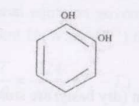
\includegraphics[width=0.7\columnwidth]{figs/ass1_i_q14_1.png}
    \caption{}
    \end{figure}

(b) \begin{figure}[H]
    \centering
    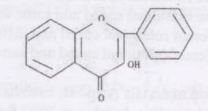
\includegraphics[width=0.7\columnwidth]{figs/ass1_i_q14_2.png}
    \caption{}
    \end{figure} 

(c) \begin{figure}[H]
    \centering
    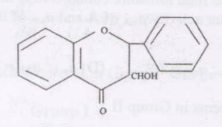
\includegraphics[width=0.7\columnwidth]{figs/ass1_i_q14_3.png}
    \caption{}
    \end{figure}

(d) \begin{figure}[H]
    \centering
    \includegraphics[width=0.7\columnwidth]{figs/ass1_i_q14_4.png}
    \caption{}
    \end{figure}
    
\end{multicols}

(GATE XE 2008)

\item The specific growth rate of \textit{Bacillus cereus} in a food sample is $0.4\ \mathrm{h}^{-1}$. Doubling time of the cell is  

\begin{enumerate}
\begin{multicols}{4}
\item  $2.0\ \mathrm{h}$ 
\item  $1.73\ \mathrm{h}$ 
\item  $1.25\ \mathrm{h}$ 
\item  $1.0\ \mathrm{h}$ 
\end{multicols}
\end{enumerate}

(GATE XE 2008)

\item Match the items in Group I with the most appropriate items in Group II
 
\begin{table}[H]     \centering     \caption{}     \label{}     \begin{tabular}{l l}

\textbf{Group I} & \textbf{Group II} \\
(P) Cheese & (1) Hydrogen peroxide \\
(Q) Enterotoxin B & (2) Nisin \\
(R) Bacteriocin & (3) \textit{Propionibacterium} \\
(S) Milk ropiness & (4) \textit{Alcaligenes} \\
 & (5) \textit{Staphylococcus aureus} \\
\end{tabular} \end{table}  

\begin{enumerate}
\begin{multicols}{2}
\item  P-5, Q-1, R-2, S-4  
\item  P-3, Q-1, R-5, S-4
\item  P-3, Q-5, R-2, S-4  
\item  P-3, Q-5, R-2, S-1 
\end{multicols}
\end{enumerate}

(GATE XE 2008)

\item Five grams of cheese was mixed with $45\ \mathrm{ml}$ of sterile diluent. Two successive dilutions of 1:100 each were made and one-tenth milliliter from the last dilution was plated onto each of two plates containing plate count agar (PCA) medium. Following incubation, $56$ colonies were counted on one plate and $54$ on the other. The average number of colony forming units (CFUs) per gram of cheese is

\begin{enumerate}
\begin{multicols}{4}
\item  $5.5 \times 10^5$  
\item  $5.5 \times 10^6$  
\item  $5.5 \times 10^7$  
\item  $5.5 \times 10^8$ 
\end{multicols}
\end{enumerate}

(GATE XE 2008)

\item Match the items in Group I with the most appropriate items in Group II  

\begin{table}[H]     \centering     \caption{}     \label{}     \begin{tabular}{l l}

\textbf{Group I} & \textbf{Group II} \\
(P) Spore former & (1) \textit{Listeria} \\
(Q) Vinegar & (2) \textit{Shigella} \\
(R) Psychrotroph & (3) \textit{Lactobacillus} \\
(S) Dysentery & (4) \textit{Bacillus} \\
 & (5) \textit{Acetobacter} \\
\end{tabular} \end{table}  

\begin{enumerate}
\begin{multicols}{2}
\item  P-3, Q-5, R-4, S-2  
\item  P-4, Q-5, R-1, S-2 
\item  P-4, Q-5, R-1, S-3  
\item  P-4, Q-3, R-1, S-2 
\end{multicols}
\end{enumerate}

(GATE XE 2008)

\item Development of ‘hot spot’ in high moisture grain during storage in silo is due to  

\begin{enumerate}
\item  exothermic reaction between moisture and starch present in the endosperm of the grain 
\item  microbial growth and respiration of grain 
\item  heating of the silo wall during day and cooling during night 
\item  exothermic reaction between the moisture present in endosperm and the oil in germ 
\end{enumerate}

(GATE XE 2008)

\item In modern rice mills, the two rubber rolls in the sheller rotate in opposite direction at the  

\begin{enumerate}
\item  same rotational speed and different surface speed 
\item  same rotational speed and same surface speed  
\item  different rotational speed and different surface speed  
\item  different rotational speed and same surface speed  
\end{enumerate}

(GATE XE 2008)  

\item Two food materials A and B, each having $14\%$ moisture content (dry basis) are stored in a constant relative humidity chamber at $30^{\circ} \mathrm{C}$ for equilibration. The final moisture contents of A and B are $6\%$ and $12\%$ (both in dry basis), respectively. The final water activity $a_{wA}$ of A and $a_{wB}$ of B are related as  

\begin{enumerate}
\begin{multicols}{4}
\item  $a_{wA} : a_{wB} =$\newline$ 0.65 : 1$  
\item  $a_{wA} : a_{wB} =$\newline$ 1 : 1$  
\item  $a_{wA} : a_{wB} = $\newline$1 : 2$  
\item  $a_{wA} : a_{wB} =$\newline$ 2 : 1$ 
\end{multicols}
\end{enumerate}

(GATE XE 2008)  

\item Match the items in Group I with the most appropriate items in Group II  

\begin{table}[H]     \centering     \caption{}     \label{}     \begin{tabular}{p{7cm} p{7cm}}
\textbf{Group I} & \textbf{Group II} \\
(P) Disc centrifuge & (1) Separation of solid phase in milk by coagulation \\
(Q) Multiple effect evaporator & (2) Aseptic packaging of milk \\
(R) UHT processing & (3) Separation of liquid phases in milk \\
(S) Homogenization & (4) Dispersion of one of the liquid phases in milk \\
& (5) Concentration of milk \\
\end{tabular} \end{table}  

\begin{enumerate}
\begin{multicols}{2}
\item  P-3, Q-5, R-1, S-4  
\item  P-1, Q-5, R-2, S-4  
\item  P-3, Q-5, R-2, S-1  
\item  P-3, Q-5, R-2, S-4  
\end{multicols}
\end{enumerate}

(GATE XE 2008)  

\item Rigor mortis in meat is due to  

\begin{enumerate}
\item  glycolysis followed by formation of lactic acid  
\item  binding of collagen and elastin  
\item  action of cathepsin enzyme in meat  
\item  binding of myosin and actin  
\end{enumerate}

(GATE XE 2008)  

\item Following operations are adopted for cleaning in place (CIP) of equipment  

P: Cold water rinse; Q: Hot water rinse; R: Alkali cleaning; S: Acid cleaning  

The correct sequence of CIP for equipment used in UHT processing of milk is  

\begin{enumerate}
\begin{multicols}{2}
\item  P – Q – R – S – P  
\item  P – Q – R – Q – S – P  
\item  P – Q – R – Q – S – P  
\item  P – Q – S – P  
\end{multicols}
\end{enumerate}

(GATE XE 2008)  

\item Following operations are adopted for refining of vegetable oils  

P: Winterization; Q: Alkali refining; R: Steam deodorization; S: Bleaching; T: Degumming  

The correct sequence of operations for the refining is  

\begin{enumerate}
\begin{multicols}{2}
\item  P – Q – T – R – S  
\item  S – R – Q – T – P  
\item  Q – T – S – R – P  
\item  R – T – Q – S – P  
\end{multicols}
\end{enumerate}

(GATE XE 2008)  

\item A liquid having density $\rho$ and viscosity $\mu$ flows under laminar condition through a circular pipe having diameter $D$ and length $L$ against a pressure drop of $\Delta P$. Volume flow rate of the liquid through the pipe will be proportional to  

\begin{enumerate}
\begin{multicols}{4}
\item  $\dfrac{D^4 \Delta P}{\mu L}$  
\item  $\dfrac{D^3 \Delta P}{\mu L}$  
\item  $\dfrac{D \Delta P}{\mu L}$  
\item  $\dfrac{\Delta P}{\mu L}$  
\end{multicols}
\end{enumerate}

(GATE XE 2008)  

\item  A liquid having mass $M$ (kg), heat capacity $C_p$ (J.kg$^{-1} \, ^\circ$C$^{-1}$) is cooled in an agitated vessel having surface area $A$ (m$^2$). A cooling medium at temperature $T_r$ ($^\circ$C) is used for cooling the liquid. The differential equation governing the temperature change $\frac{dT}{d\theta}$ of liquid with overall heat transfer coefficient $U$ (W.m$^{-2} \, ^\circ$C$^{-1}$) for the vessel is given by  

\begin{enumerate}
\begin{multicols}{2}
\item  $\frac{dT}{d\theta} = \frac{UA}{MC_p} (T_r - T)$  
\item  $\frac{dT}{d\theta} = \frac{MC_p}{UA} (T_r - T)$  
\item  $\frac{dT}{d\theta} = \frac{MC_p}{UA} (T_r - T)$  
\item  $\frac{dT}{d\theta} = \frac{UA}{MC_p} (T_r - T)$  
\end{multicols}
\end{enumerate}

(GATE XE 2008)  

\item  Match the items in Group I with the most appropriate items in Group II  

\begin{table}[H]     \centering     \caption{}     \label{}     \begin{tabular}{p{7cm} p{7cm}}
\textbf{Group I} & \textbf{Group II} \\
(P) Freezing & (1) Stoke's law \\
(Q) Fat globules movement in milk & (2) Plank's equation \\
(R) Flow through packed bed & (3) Ergun's equation \\
(S) Boiling temperature & (4) Hagen Poiseulli's equation \\
& (5) Raoult's law \\
\end{tabular} \end{table}  

\begin{enumerate}
\begin{multicols}{2}
\item  P-4, Q-1, R-3, S-5  
\item  P-2, Q-1, R-3, S-4  
\item  P-2, Q-1, R-4, S-5  
\item  P-2, Q-1, R-3, S-5 
\end{multicols}
\end{enumerate}
(GATE XE 2008)  

\item[] \textbf{\Large Common Data Questions}

\textbf{Common Data for Questions 29 and 30:} 

Milk having heat capacity $3900$ J.kg$^{-1} \, ^\circ$C$^{-1}$ and density $1020$ kg.m$^{-3}$ is pressurized to 300 atmosphere gauge pressure and allowed to flow through a high pressure homogenizing valve at a rate of 60 liters per min. The diameter of the homogenizing valve through which the milk flows is 6 mm. (1 atmosphere = 101.3 kPa)  

\item Temperature rise in milk will be  

\begin{enumerate}
\begin{multicols}{4}
\item  $10.1 \, ^\circ$C  
\item  $9.2 \, ^\circ$C  
\item  $7.7 \, ^\circ$C  
\item  $6.1 \, ^\circ$C  
\end{multicols}
\end{enumerate}

(GATE XE 2008)  

\item Height of the valve lift will be  

\begin{enumerate}
\begin{multicols}{4}
\item  $0.06$ mm  
\item  $0.11$ mm  
\item  $0.16$ mm  
\item  $0.22$ mm  
\end{multicols}
\end{enumerate}

(GATE XE 2008)  

\item[] \textbf{\Large Linked Answer Questions: Q.31 to Q.34 carry two marks each.}

  
\textbf{ Statement for Linked Answer Questions 31 and 32:  }
A medium acid food is sterilized at $100^\circ$C in a can to reduce the number of heat resistant organisms ($D_{120} = 2$ min, $z = 10^\circ$C) from an initial count of $10000$ per can to a probability of survival of $1$ in million.  

\item $D_{100}$ value of this organism is 

\begin{enumerate}
\begin{multicols}{4}
\item  $0.4$ min  
\item  $20$ min  
\item  $4$ min  
\item  $10$ min  
\end{multicols}
\end{enumerate}

(GATE XE 2008)  

\item The total processing time is  

\begin{enumerate}
\begin{multicols}{4}
\item  $100$ min  
\item  $40$ min  
\item  $200$ min  
\item  $4$ min  
\end{multicols}
\end{enumerate}

(GATE XE 2008)  

\item[] \textbf{Statement for Linked Answer Questions 33 and 34:}

Compressed air at 0.5 atmosphere gauge pressure and 30$^\circ$C contains 0.01 kg water vapor per kg dry air. Molecular weight of dry air and water vapor are 28.9 and 18 kg.kmol$^{-1}$, respectively. Saturation vapor pressure of water at 30$^\circ$C is 4.246 kPa absolute. (1 atmosphere = 101.3 kPa) \\

\item Partial pressure of water vapor inside the compressor is 

\begin{enumerate}
\begin{multicols}{4}
\item  2.15 kPa 
\item  2.40 kPa 
\item  3.12 kPa 
\item  3.51 kPa 
\end{multicols}
\end{enumerate}

(GATE XE 2008)

\item Relative humidity of air inside the compressor is

\begin{enumerate}
\begin{multicols}{4}
\item  40.1\%  
\item  49.8\% 
\item  56.5\% 
\item  57.6\%
\end{multicols}
\end{enumerate}

(GATE XE 2008)

\end{enumerate}

\begin{center}
    \textbf{END OF SECTION - I}
\end{center}

\end{document}

